\def\catalan{0}
\def\coloring{0}
\documentclass[a4paper,UKenglish,cleveref,autoref]{lipics-v2019}

\usepackage[dvipsnames]{xcolor}
\hypersetup{
    colorlinks=true,
    linkcolor=BrickRed,
    linkbordercolor=BrickRed,
    citecolor=OliveGreen,
    citebordercolor=OliveGreen,
    urlcolor=RoyalBlue}

\usepackage[noend]{algpseudocode}
\usepackage{algorithm}
\usepackage{algorithmicx}
\usepackage{thm-restate}
\usepackage{mathtools}
\usepackage[colorinlistoftodos]{todonotes}
\usepackage[T1]{fontenc}
\usepackage{relsize}
%\usepackage{multirow}
\usetikzlibrary{
  shapes.multipart,
  matrix,
  positioning,
  shapes.callouts,
  shapes.arrows,
  calc}


\def\bo{\mathcal{O}}
\def\Bo{\mathlarger{\mathcal{O}}}
\def\bt{\Theta}
\def\polylog{\mathrm{polylog}\;}

\DeclarePairedDelimiter\floor{\lfloor}{\rfloor}
\newcommand{\func}[1]{\texttt{\textsc{#1}}}
\def\poly{\mathrm{poly}}

\renewcommand\algorithmicthen{}
\renewcommand\algorithmicdo{}

\def\filled{\textup{\textsf{filled}}}
\def\unfilled{\textup{\textsf{unfilled}}}

\def\ZERO{\mathsf{0}}
\def\ONE{\mathsf{1}}
\def\PHI{\phi}
\def\LAST{\mathbf{last}}
\def\BUCKET{\mathbf{bucket}}
\def\BEGIN{\mathbf{begin}}
\def\END{\mathbf{end}}
\def\ADJ{\mathbf{A}}

\newcommand{\sectioninput}{\input}
\newcommand{\BD}{$\widetilde{\mathcal O}(1)$}
\newcommand{\ROPL}{$r\cdot \log^{\mathcal O(1)} n$}
\newcommand{\OPL}{$\log^{\mathcal O(1)} n$}
\newcommand{\RPL}[1]{
    \ifnum1=#1\relax
        $r\cdot \log n$
    \else
        $r\cdot \log^{#1} n$
    \fi
}
\newcommand{\PL}[1]{
    \ifnum1=#1\relax
        $\log n$
    \else
        $\log^{#1} n$
    \fi
}
\newcommand{\UBD}{$\times$}
\newcommand{\hagu}{k}
\newcommand{\thicksquare}{\tikz[baseline]\draw[very thick](0,0)rectangle(0.2,0.2);}

\usepackage{bm}
\usepackage{wrapfig, framed, caption}
\usepackage{footmisc}
\usepackage[parfill]{parskip}
\usepackage{soul}
\sethlcolor{Red!20}

\renewcommand{\vec}[1]{\mathbf{#1}}
\graphicspath{{./images/}}

\theoremstyle{plain}
\newtheorem{invariant}[theorem]{Invariant}


\bibliographystyle{alpha}

\title{Local Access to Huge Random Objects through Partial Sampling}

\date{}
\author{Amartya Shankha Biswas}{CSAIL, MIT}{asbiswas@mit.edu}{https://orcid.org/0000-0002-5068-1524}{funding}
\author{Ronitt Rubinfeld}{CSAIL, MIT}{ronitt@csail.mit.edu}{}{funding}
\author{Anak Yodpinyanee}{CSAIL, MIT}{anak@csail.mit.edu}{https://orcid.org/0000-0002-7572-2003}{funding}

\authorrunning{A.\,S. Biswas}

\keywords{Dummy keyword}%TODO mandatory; please add comma-separated list of keywords

\nolinenumbers

\hideLIPIcs


\begin{document}

\maketitle

\begin{abstract}

\todo[inline,color=red!80!green!25]{Talk about enhanced model}
Consider an algorithm performing a computation on a \emph{huge random object} (for example a random graph or a ``long'' random walk).
Is it necessary to generate the entire object prior to the computation,
or is it possible to provide query access to the object and sample it incrementally ``on-the-fly'' (as requested by the algorithm)?
Such an \emph{implementation} should emulate the random object by answering queries in a manner consistent with
an instance of the random object sampled from the true distribution (or close to it).
This paradigm is useful when the algorithm is sub-linear and thus, sampling the entire object up front would ruin its efficiency.

Our first set of results focus on undirected graphs with independent edge probabilities,
i.e. each edge is chosen as an independent Bernoulli random variable.
We provide a general implementation for this model under certain assumptions.
Then, we use this to obtain the first efficient local implementations for the Erd\"os-R\'enyi $G(n,p)$ model for \emph{all} values of $p$,
and the Stochastic Block model.
As in previous local-access implementations for random graphs, we support \func{Vertex-Pair} and \func{Next-Neighbor} queries.
In addition, we introduce a new \func{Random-Neighbor} query.
Next, we give the first local-access implementation for \func{All-Neighbors} queries in the (sparse and directed) Kleinberg's Small-World model.
Our implementations require no pre-processing time, and answer each query using $ \mathcal{O}(\poly(\log n)) $ time, random bits, and additional space.

Next, we show how to implement random Catalan objects, specifically focusing on Dyck paths
(balanced random walks on the integer line that are always positive).
Here, we support $\func{Height}$ queries to find the location of the walk,
and $\func{First-Return}$ queries to find the time when the walk returns to a specified location.
This in turn can be used to implement $\func{Next-Neighbor}$ queries on random rooted and binary trees,
and $\func{Matching-Bracket}$ queries on random well bracketed expressions (the Dyck language).

Finally, we study random $q$-colorings of graphs with max degree $\Delta$.
In contrast to the prior settings, where random objects are generated according to a single distribution with $\mathcal O(1)$ parameters
(for example, $n$ and $p$ in the $G(n,p)$ model), the distribution here is specified via a ``huge'' input (in this case, the underlying graph).
When $q > \alpha\Delta$ for a small constant $\alpha$, we show how to answer queries to the color of any given node in sub-linear time.

\end{abstract}

\newpage

\begingroup
  %\hypersetup{hidelinks}
  \tableofcontents
\endgroup
\newpage

\section{Introduction}

The problem of computing local information of huge random objects
was pioneered in \cite{huge_old,huge}. 
Further work of \cite{sparse} considers the generation of sparse random $G(n,p)$ graphs
from the Erd\"{o}s-R\'{e}nyi model \cite{er}, with $p = O(\poly(\log n)/n)$,
which answers $\poly(\log n)$ \func{All-Neighbors} queries,
listing the neighbors of queried vertices.
While these generators use polylogarithmic resources over their entire execution, 
they generate graphs that are  only guaranteed to {\em appear random} to algorithms
that inspect a {\em limited portion} of the generated graph.

In \cite{reut}, the authors construct an oracle for the generation of recursive trees,
and BA preferential attachment graphs.
Unlike \cite{sparse}, their implementation allows for an arbitrary number of queries.
This result is particularly interesting --  
although the graphs in this model are generated via a sequential process,
the oracle is able to locally generate arbitrary portions of it
and answer queries in polylogarithmic time.
Though preferential attachment graphs are sparse,
they contain vertices of high degree,
thus \cite{reut} provides access to 
the adjacency list through \func{Next-Neighbor} queries.
%On a high level, this is due to the fact that the BA model is directed, and all edges are independent.

In this work, we begin by \emph{formalizing} a model of local-access generators
implicitly used in \cite{reut}.
We next construct oracles that allow queries to both the adjacency matrix
and adjacency list representation of a basic class of random
graph families, without generating the entire graph at the onset.
Our oracles
provide \func{Vertex-Pair}, \func{Next-Neighbor}, and \func{Random-Neighbor} queries\footnote{\func{Vertex-Pair}$(u,v)$ returns whether $u$ and $v$ are adjacent, \func{Next-Neighbor}$(v)$ returns a new neighbor of $v$ each time it is invoked (until none is left), and \func{Random-Neighbor}$(v)$ returns a uniform random neighbor of $v$ (if $v$ is not isolated).}
for graphs with {\em independent edge probabilities}, that is,
when each edge is chosen as an independent Bernoulli random variable. 
Using this framework, we construct the first \emph{efficient} local-access generators for undirected graph models, supporting all three types of queries
using $\mathcal{O}(\poly(\log n))$ time, space, and random bits
per query, under assumptions on the ability to compute certain values
pertaining to consecutive edge probabilities. In particular, our construction yields local-access generators for the Erd\"{o}s-R\'{e}nyi $G(n,p)$ model (for \emph{all} values of $p$), and the Stochastic Block model with random community assignment. 
As in \cite{reut} (and unlike the generators in \cite{huge_old,huge,sparse}), 
our techniques allow unlimited queries.%(i.e. the entire graph can be generated).

While \func{Vertex-Pair} and \func{Next-Neighbor} queries, as well as \func{All-Neighbors} queries for sparse graphs, have been considered in the prior works of \cite{reut, huge_old, huge, sparse}, we provide the first implementation (to the best of our knowledge)
of \func{Random-Neighbor} queries, which do not follow trivially from the
\func{All-Neighbor} queries in \emph{non-sparse graphs}.
Such queries are useful, for instance, for sub-linear algorithms that employ random walk processes.
\func{Random-Neighbor} queries
present particularly interesting challenges,  since as we note in 
Section~\ref{par:random_neighbor_queries},
(1) \func{Random-Neighbor} queries affect the conditional probabilities
of the remaining neighbors in a non-trivial manner, and
(2) our implementation does not resort to explicitly sampling the degree of any vertex in order to generate a random neighbor.
First, sampling the degree of the query vertex, we suspect, is not viable for \emph{sub-linear} generators,
because this quantity alone imposes dependence on the existence of \emph{all} of its potential incident edges.
Therefore, our generator needs to return a random neighbor, with probability reciprocal to the query vertex's degree,
without resorting to ``knowing'' its degree.
Second, even without committing to the degrees, answers to \func{Random-Neighbor} querie
affect the conditional probabilities of the remaining adjacencies in a global and non-trivial manner
-- that is, from the point of view of the \emph{agent} interacting with the generator.
The generator, however, must somehow maintain and leverage its additional \emph{internal knowledge}
of the partially-generated graph, to keep its computation tractable throughout the entire graph generation process.

We then consider local-access generators for directed graphs in Kleinberg's Small World model.
In this case, the probabilities are based on distances in a 2-dimensional grid.
Using a modified version of our previous sampling procedure,
we present such a generator supporting \func{All-Neighbors} queries in 
$\mathcal{O}(\poly(\log n))$ time, space and random bits per query (since such graphs
are sparse, the other queries follow directly).

For additional related work, see Section~\ref{sec:related_work}.




\section{Our Contributions and Techniques}

We begin by formalizing a model of {\em local-access generators}
(Section~\ref{sec:oracle_model}), implicitly used in \cite{reut}.
Our work provides local-access generators for various
basic classes of graphs described in the following, with 
\func{Vertex-Pair}, \func{Next-Neighbor}, and \func{Random-Neighbor}
queries.  In all of our results,
each query is processed using $\poly(\log n)$
time, random bits, and additional space, with \emph{no initialization overhead}.
These guarantees hold even in the case of adversarial queries.
Our bounds assume constant computation time for each arithmetic operation with
$O(\log n)$-bit precision. Each of our generators constructs a random graph
drawn from a distribution that is $1/\poly(n)$-close
to the desired distribution in the $L_1$-distance.\footnote{The \emph{$L_1$-distance} between two probability distributions $\distr{p}$
and $\distr{q}$ over domain $D$ is defined as $\|\distr{p-q}\|_1 = 
\sum_{x \in D } |p(x)-q(x)|$.
We say that $\distr{p}$ and $\distr{q}$ are $\epsilon$-close if $\|\distr{p-q}\|_1 \leq \epsilon$.
%Note that the \emph{total variation distance} is related to the $L_1$-distance as $d_{\mathrm{TV}}(\matr{p},\matr{q})=\frac{1}{2}\|\distr{p-q}\|_1$.
}



\subsection{Undirected Graphs}
\label{sec:undirected_graphs}
In Section~\ref{sec:undirected} we construct local access generators for the generic
class of undirected graphs
with {\em independent edge probabilities} $\left\{ p_{u,v} \right\}_{u,v\in V}$,
where $p_{u,v}$ denote the probability that there is an edge between $u$ and $v$.
Throughout, we identify our vertices via their unique IDs from $1$ to $n$, namely $V = [n]$.
We assume that we can compute various values pertaining to consecutive
edge probabilities for the class of graphs, as detailed below.
We then show that such values can be computed for graphs
generated according to the Erd\"{o}s-R\'{e}nyi $G(n,p)$ model
and the Stochastic Block model.

\paragraph*{\func{Next-Neighbor} Queries}
\label{par:next_neighbor_queries}
We note that the next neighbor of a vertex can be found trivially by generating consecutive
entries of the adjacency matrix, but for small edge probabilities $p_{u,v} = o(1)$
this implementation can be too slow.  In our algorithms, we achieve speed-up by sampling multiple 
neighbor values at once for a given vertex $u$; more specifically,  
we sample for the number of ``non-neighbors'' preceding
the next neighbor.
To do this, we assume that we have access to
an oracle which can estimate the ``skip'' probabilities 
$F(v,a,b)=\prod^{b}_{u=a} (1-p_{v,u})$,
where $F(v,a,b)$ is the probability that $v$ 
has no neighbors in the range $[a,b]$.
We later show that it is possible to compute this quantity efficiently
for the $G(n,p)$ and Stochastic block models.

A main difficulty in our setup, as compared to \cite{reut},
arises from the fact that our graph is undirected, and thus
we must design a data structure that ``informs'' all (potentially $\Theta(n)$) non-neighbors once we decide on the query vertex's next neighbor.
%Unlike in the case of directed graphs, each $\func{Next-Neighbor}$ query
%can affect the probabilities of a large number of other vertices.
More concretely, if $u'$ is sampled as the next neighbor of $v$ after its previous neighbor $u$,
we must maintain consistency in subsequent steps
by ensuring that none of the vertices in the range $(u,u')$
return $v$ as a neighbor. This update will become even more complicated as we later handle \func{Random-Neighbor} queries, where we may generate non-neighbors at random locations.

In Section~\ref{sec:ER-rand}, we present a very simple randomized generator
(Algorithm~\ref{alg:oblivious-coin-toss}) that supports \func{Next-Neighbor}
queries efficiently, albeit the analysis of its performance is rather complicated.
We remark that this approach may be extended to support \func{Vertex-Pair} queries with superior performance (given that we do not to support \func{Random-Neighbor} queries) and to provide deterministic resource usage guarantee -- the full analysis can be found in Section~\ref{sec:reroll-cont} and \ref{sec:ER-det}, respectively.

\paragraph*{\func{Random-Neighbor} Queries}
\label{par:random_neighbor_queries}
We provide efficient \func{Random-Neighbor} queries (Section~\ref{sec:buckets}).
The ability to do so is surprising.  First, note that after performing a \func{Random-Neighbor} query
all other conditional probabilities will be affected in a non-trivial way.
\footnote{Consider a $G(n,p)$ graph with small $p$, say $p = 1/\sqrt n$,
such that vertices will have $\tilde{\mathcal{O}}(\sqrt n)$ neighbors with high probability.
After $\tilde{\mathcal{O}}(\sqrt n)$ \func{Random-Neighbor} queries,
we will have uncovered all the neighbors (w.h.p.),
so that the conditional probability of the remaining
$\Theta(n)$ edges should now be close to zero.}
This requires a way of implicitly keeping track of all the resulting changes.
Second, we can sample a \func{Random-Neighbor} with the correct probability $1/\deg(v)$,
even though we do not sample or know the degree of the vertex.

We formulate a {\em bucketing approach} (Section~\ref{sec:buckets})
which samples multiple consecutive edges at once, in such a way
that the conditional probabilities of the unsampled edges
remain independent and ``well-behaved'' during subsequent queries.
For each vertex $v$, we divide the vertex set (potential neighbors) or $v$ into consecutive ranges (buckets),
so that each bucket contains, in expectation, roughly the same number of neighbors
$\sum^{b}_{u=a} p_{v,u}$ (which we must be able to compute efficiently).
The subroutine of \func{Next-Neighbor} may be applied to sample the neighbors within a bucket in expected constant time.
Then, one may obtain a random neighbor of $v$ by picking a random neighbor from a random bucket;
probabilities of picking any neighbors may be normalized to the uniform distribution via rejection sampling,
while stilling yielding $\poly(\log n)$ complexities overall.
This bucketing approach also naturally leads to our data structure that requires
constant space for each bucket and for each edge, using $\Theta(n+m)$ overall memory requirement.
The \func{Vertex-Pair} queries are implemented by sampling the relevant bucket.

We now consider the application of our construction above to actual random graph models,
where we must realize the assumption that $\prod^{b}_{u=a} (1-p_{v,u})$
and $\sum^{b}_{u=a} p_{v,u}$ can be computed efficiently.
This holds trivially for the $G(n,p)$ model via closed-form formulas,
but requires an additional back-end data structure for the Stochastic Block models.

\paragraph*{Erd\"{o}s-R\'{e}nyi}
\label{par:erdos_renyi}
In Section~\ref{sec:app_er}, we apply our construction to random $G(n,p)$ graphs for
arbitrary $p$, and obtain
$\func{Vertex-Pair}$, $\func{Next-Neighbor}$, and $\func{Random-Neighbor}$ queries,
using polylogarithmic resources (time, space and random bits) per query.
We remark that, while $\Omega(n+m) = \Omega(p n^2)$ time and space
is clearly necessary to generate and represent a full random graph,
our implementation supports local-access via all three types of queries, 
and yet can generate a full graph in $\widetilde{O}(n+m)$ time and space (Corollary~\ref{thm:er-optimal}),
which is tight up to polylogarithmic factors.

%{\color{red}
\paragraph*{Stochastic Block Model}
\label{par:stochastic_block_model}
We generalize our construction to the Stochastic Block Model.
In this model, the vertex set is partitioned into $r$ \emph{communities}
$\left\{ C_1, \ldots, C_r \right\}$.
The probability that an edge exists depends on the communities of its endpoints:
if $u\in C_i$ and $v \in C_j$, then $\{u,v\}$ exists with probability $p_{i,j}$,
given in an $r\times r$ matrix $\matr{P}$.
As communities in the observed data are generally unknown a priori,
and significant research has been devoted to designing efficient algorithm
for community detection and recovery,
these studies generally consider the \emph{random community assignment} condition for the purpose of designing and analyzing algorithms (see e.g., \cite{mossel2015reconstruction}).
Thus, in this work, we aim to construct generators for this important case, where the community assignment of vertices are independently sampled from some given distribution $\distr{R}$.
%}

Our approach is, as before, to sample for the next neighbor or a random neighbor directly,
although our result does not simply follow closed-form formulas,
as the probabilities for the potential edges now depend
on the communities of endpoints.
To handle this issue, we observe that it is sufficient to efficiently count
the number of vertices of each community in any
range of contiguous vertex indices.
We then design a data structure extending a construction of \cite{huge},
which maintain these counts for ranges of vertices,
and ``sample'' the partition of their counts only on an as-needed basis.
This extension results in an efficient technique to sample counts
from the \emph{multivariate hypergeometric distribution} (Section~\ref{sec:multivariate_hypergeometric_sampling}).
This sampling procedure may be of independent interest.
For $r$ communities, this yields an implementation with
$ \mathcal{O}(r\cdot \poly(\log n))$ overhead in required resources for each operation.
This upholds all previous polylogarithmic guarantees when $r = \poly(\log n)$.

\paragraph*{CDF Based Sampling}
It is worth noting that our techniques for implementing local-access for the ER and SBM graphs
can easily be extended to other similar models of random graphs.
The only requirement is that the CDF of the probability sequences can be efficiently computed as in Section~\ref{para:CDF}.





\subsection{Directed Graphs}
\label{sec:directed_graphs}
Lastly, we consider Kleinberg's Small World model (\cite{kleinberg, klein}) in Section~\ref{sec:small_world}.
While Small-World models are proposed to capture 
properties of observed data such as small shortest-path 
distances and large clustering coefficients \cite{watts1998collective}, 
this important special case of Kleinberg's model, defined on two-dimensional grids, 
demonstrates underlying geographical structures of networks. 
The vertices are aligned on a $\sqrt{n}\times\sqrt{n}$ grid,
and the edge probabilities are a function of a two-dimensional distance metric.
Since the degree of each vertex in this model is $\Bo(\log n)$ with high probability,
we design generators supporting \func{All-Neighbor} queries.
%In contrast to our previous cases, this model imposes an underlying
%two-dimensional structure of the vertex set, which governs
%the distance function as well as complicates the individual edge probabilities.

\section{Our Contributions and Techniques}
\label{sec:our_contributions_and_techniques}

The problem of computing local information of huge random objects was pioneered in \cite{huge_old,huge}.
Further work of \cite{sparse} considers the generation of sparse random $G(n,p)$ graphs from the Erd\"{o}s-R\'{e}nyi model \cite{er},
with $p = O(\poly(\log n)/n)$, which answers $\poly(\log n)$ \func{All-Neighbors} queries, listing the neighbors of queried vertices.
While these implementations use polylogarithmic resources over their entire execution,
they generate graphs that are  only guaranteed to {\em appear random} to algorithms that inspect a {\em limited portion} of the generated graph.
For example, the greedy routing algorithm on Kleinberg's small world networks \cite{kleinberg} only uses $\mathcal O(\log^2 n)$ probes.
Using our implementation, one can execute this algorithm on a random small world instance
in $\mathcal O(\poly(\log n))$ time without incurring the $\mathcal O(n)$ prior-sampling overhead.

In \cite{reut}, the authors construct an oracle for the generation of recursive trees, and BA preferential attachment graphs.
Unlike \cite{sparse}, their implementation allows for an arbitrary number of queries.
This result is particularly interesting --  although the graphs in this model are generated via a sequential process,
the oracle is able to locally generate arbitrary portions of it and answer queries in polylogarithmic time.
Though preferential attachment graphs are sparse, they contain vertices of high degree,
thus \cite{reut} provides access to the adjacency list through \func{Next-Neighbor} queries.




\section{Preliminaries}
\label{sec:model}
\subsection{Local-Access Generators}
\label{sec:oracle_model}

We begin by formalizing a model of {\em local-access generators} (Section~\ref{sec:oracle_model}), implicitly used in \cite{reut}.
\todo{Not good}
Our work provides local-access generators for various basic classes of graphs described in the following, with 
\func{Vertex-Pair}, \func{Next-Neighbor}, and \func{Random-Neighbor} queries.
In all of our results, each query is processed using $\poly(\log n)$ time, random bits, and additional space, with \emph{no initialization overhead}.
These guarantees hold even in the case of adversarial queries.
Our bounds assume constant computation time for each arithmetic operation with $O(\log n)$-bit precision.
Each of our generators constructs a random graph drawn from a distribution that is $1/\poly(n)$-close to the desired distribution in the $L_1$-distance.
\footnote{The \emph{$L_1$-distance} between two probability distributions $\distr{p}$ and $\distr{q}$ over domain $D$
is defined as $\|\distr{p-q}\|_1 = \sum_{x \in D } |p(x)-q(x)|$.
We say that $\distr{p}$ and $\distr{q}$ are $\epsilon$-close if $\|\distr{p-q}\|_1 \leq \epsilon$.}

We consider the problem of locally generating random graphs $G = (V,E)$ drawn from the desired families of simple unweighted graphs, undirected or directed. We denote the number of vertices $n = |V|$, and refer to each vertex simply via its unique ID from $[n]$. For undirected $G$, the set of neighbors of $v \in V$ is defined as $\Gamma(v) = \{u \in V: \{v,u\} \in E\}$; denote its degree by $\deg(v) = |\Gamma(v)|$.
Inspired by the goals and results of \cite{reut}, we define a model of local-access generators as follows.
\begin{definition}
A \emph{local-access generator} of a random graph $G$ sampled from a distribution $\distr{D}$,
is a data structure that provides access to $G$ by answering various types of
\emph{supported queries}, while satisfying the following:
%For clarity, we assume that the generator is invoked until its entire graph $G$ is exposed.
%The local-access generator for a probability distribution $\distr{D}$ of the desired random graph model must satisfy the following properties:
\begin{itemize}
\item \textbf{Consistency.} The responses of the local-access generator to all probes throughout the entire execution must be consistent with a single graph $G$.
\item \textbf{Distribution equivalence.} 
The random graph $G$ provided by the generator must be sampled from some distribution $\distr{D}'$
that is $\epsilon$-close to the desired distribution $\distr{D}$ in the $L_1$-distance.
In this work we focus on supporting $\epsilon = n^{-c}$ for any desired constant $c>0$.
As for \func{Random-Neighbor}$(v)$, the distribution from which a neighbor is returned
must be $\epsilon$-close to the uniform distribution over neighbors of $v$
with respect to the sampled random graph $G$ (w.h.p $1-n^{-c}$ for each query).
\item \textbf{Performance.} The resources, consisting of (1) computation time, (2) additional random bits required, and (3) additional space required, in order to compute an answer to a single query and update the data structure, must be sub-linear, preferably $\poly(\log n)$.
\end{itemize}
\end{definition}
In particular, we allow queries to be made adversarially and non-deterministically. The adversary has full knowledge of the generator's behavior and its past random bits.

For ease of presentation, we allow generators to create graphs with self-loops.
When self-loops are not desired, it is sufficient to add a wrapper function that simply re-invokes \func{Next-Neighbor}$(v)$ or \func{Random-Neighbor}$(v)$ when the generator returns $v$.


\paragraph*{Supported Queries in our Model} 
For undirected graphs, we consider queries of the following forms.
now we might want to do \func{Next-Neighbor} first for consistency.
\begin{itemize}
\item \func{Next-Neighbor}$(v)$: The generator returns the neighbor of $v$ with the lowest ID that has not been returned during the execution of the generator so far. If all neighbors of $u$ have already been returned, the generator returns $n+1$.
\item \func{Random-Neighbor}$(v)$: The generator returns a neighbor of $v$ uniformly at random (with probability $1/\deg(v)$ each). If $v$ is isolated, $\bot$ is returned.
\item \func{Vertex-Pair}$(u,v)$: The generator returns either $\ONE$ or $\ZERO$, indicating whether $\{u,v\}\in E$ or not.
\item \func{All-Neighbors}$(v)$: The generator returns the entire list of out-neighbors of $v$. We may use this query for relatively sparse graphs, specifically in the Small-World model.
\end{itemize}

\subsection{Random Graph Models}
\label{sec:graph_model}

\paragraph*{Erd\"{o}s-R\'{e}nyi Model}
We consider the $G(n, p)$ model: each edge $\{u,v\}$ exists independently with probability $p \in [0, 1]$.
Note that $p$ is not assumed to be constant, but may be a function of $n$.

\paragraph*{Stochastic Block Model}
This model is a generalization of the Erd\"{o}s-R\'{e}nyi Model. The vertex set $V$ is partitioned into $r$ communities $C_1, \ldots, C_r$. The probability that the edge $\{u,v\}$ exists is $p_{i,j}$ when $u\in C_i$ and $v\in C_j$, where the probabilities are given as an $r\times r$ symmetric matrix $\matr{P} = [p_{i,j}]_{i,j \in [r]}$.
We assume that we are given explicitly the distribution $\distr{R}$ over the communities, and
each vertex is assigned its community according to $\distr{R}$ independently at random.\footnote{Our algorithm also supports the alternative specification where the community sizes $\langle |C_1|, \ldots, |C_r|\rangle$ are given instead, where the assignment of vertices $V$ into these communities is chosen uniformly at random.}
%The main difficulty here is being able to compute the uniformly sampled assignment of vertices to communities on-the-fly.

\paragraph*{Small-World Model}
In this model, each vertex is identified via its 2D coordinate $v = (v_x, v_y) \in [\sqrt{n}]^2$. Define the Manhattan distance as $\func{dist}(u,v)=|u_x-v_x|+|u_y-v_y|$, and the probability that each directed edge $(u,v)$ exists is $c/(\func{dist}(u,v))^{2}$. Here, $c$ is an indicator of the number of long range directed edges present at each vertex. A common choice for $c$ is given by normalizing the distribution so that there is exactly one directed edge emerging from each vertex ($c = \Theta(1/\log n)$).
We will however support a range of values of $c=\log^{\pm\Theta(1)}n$.
While not explicitly specified in the original model description of \cite{kleinberg}, we assume that the probability is rounded down to $1$ if $c/(\func{dist}(u,v))^{2} > 1$.


\subsection{Miscellaneous}

\paragraph*{Arithmetic operations} Let $N$ be a sufficiently large number of bits required to maintain a multiplicative error of at most a $\frac{1}{\poly(n)}$ factor over $\poly(n)$ elementary computations ($+, -, \cdot, /, \exp$).\footnote{In our application of $\exp$, we only compute $a^b$ for $b \in \mathbb{Z}^+$ and $0 < a \leq 1+\Theta(\frac{1}{b})$, where $a^b = \Bo(1)$. For this, $N=\Bo(\log n)$ bits are sufficient to achieve the desired accuracy, namely an additive error of $n^{-c}$.} We assume that each elementary operation on words of size $N$ bits can be performed in constant time. Likewise, a random $N$-bit integer can be acquired in constant time. We assume that the input is also given with $N$-bit precision. %Any other non-trivial operations will be justified later.

\paragraph*{Sampling via a CDF}\label{para:CDF}
Consider a probability distribution $\distr{X}$ over $O(n)$ consecutive integers, whose cumulative distribution function (CDF) for can be computed with at most $n^{-c}$ additive error for constant $c$.
Using $\Bo(\log n)$ CDF evaluations, one can sample from a distribution that is
$\frac{1}{\poly(n)}$-close to $\distr{X}$ in $L_1$-distance.\footnote{Generate a random $N$-bit number $r$, and binary-search for the smallest domain element $x$ where $\mathbb P[X\leq x] \geq r$.}

\subsection{Undirected Graphs}
\label{sec:undirected_graphs}
In Section~\ref{sec:undirected}, we implement queries to both the adjacency matrix and adjacency list representation
for the generic class of \emph{undirected graphs} with {\em independent edge probabilities} $\left\{ p_{uv} \right\}_{u,v\in V}$,
where $p_{uv}$ denotes the probability that there is an edge between $u$ and $v$.
Throughout, we identify our vertices via their unique IDs from $1$ to $n$, namely $V = [n]$.
We implement \func{Vertex-Pair}, \func{Next-Neighbor}, and \func{Random-Neighbor}
\footnote{\func{Vertex-Pair}$(u,v)$ returns whether $u$ and $v$ are adjacent, \func{Next-Neighbor}$(v)$ returns a new neighbor of $v$ each time
it is invoked (until none is left), and \func{Random-Neighbor}$(v)$ returns a uniform random neighbor of $v$ (if $v$ is not isolated).} queries.
Under reasonable assumptions on the ability to compute certain values pertaining to consecutive edge probabilities,
our implementations support all three types of queries using $\mathcal{O}(\poly(\log n))$ time, space, and random bits.
In particular, our construction yields local-access generators for the Erd\"{o}s-R\'{e}nyi $G(n,p)$ model (for \emph{all} values of $p$),
and the Stochastic Block model with random community assignment.
As in \cite{reut} (and unlike the generators in \cite{huge_old,huge,sparse}), our techniques allow unlimited queries.

While \func{Vertex-Pair} and \func{Next-Neighbor} queries, as well as \func{All-Neighbors} queries for sparse graphs,
have been considered in the prior works of \cite{reut, huge_old, huge, sparse}, we provide the first implementation (to the best of our knowledge)
of \func{Random-Neighbor} queries, which do not follow trivially from the \func{All-Neighbor} queries in \emph{non-sparse graphs}.
Such queries are useful, for instance, for sub-linear algorithms that employ random walk processes.
\func{Random-Neighbor} queries present particularly interesting challenges that are outlined below.

\paragraph*{\func{Next-Neighbor} Queries}
\label{par:next_neighbor_queries}
We note that the next neighbor of a vertex can be found trivially by generating consecutive entries of the adjacency matrix,
but for small edge probabilities $p_{uv} = o(1)$ this implementation can be too slow.
In our algorithms, we achieve speed-up by sampling multiple neighbor values at once for a given vertex $u$; more specifically,
we sample for the number of ``non-neighbors'' preceding the next neighbor.
To do this, we assume that we have access to an oracle which can estimate the ``skip'' probabilities $F(v,a,b)=\prod^{b}_{u=a} (1-p_{v,u})$,
where $F(v,a,b)$ is the probability that $v$ has no neighbors in the range $[a,b]$.
We later show that it is possible to compute this quantity efficiently for the $G(n,p)$ and Stochastic block models.

A main difficulty in our setup, as compared to \cite{reut}, arises from the fact that our graph is undirected, and thus
we must design a data structure that ``informs'' all (potentially $\Theta(n)$) non-neighbors once we decide on the query vertex's next neighbor.
%Unlike in the case of directed graphs, each $\func{Next-Neighbor}$ query
%can affect the probabilities of a large number of other vertices.
More concretely, if $u'$ is sampled as the next neighbor of $v$ after its previous neighbor $u$,
we must maintain consistency in subsequent steps by ensuring that none of the vertices in the range $(u,u')$ return $v$ as a neighbor.
This update will become even more complicated as we later handle \func{Random-Neighbor} queries, where we may generate non-neighbors at random locations.

In Section~\ref{sec:ER-rand}, we present a very simple randomized generator (Algorithm~\ref{alg:oblivious-coin-toss})
that supports \func{Next-Neighbor} queries efficiently, albeit the analysis of its performance is rather complicated.
We remark that this approach may be extended to support \func{Vertex-Pair} queries with superior performance
(given that we do not to support \func{Random-Neighbor} queries) and to provide deterministic resource usage guarantee
\todo{What is deterministic here?}
-- the full analysis can be found in Section~\ref{sec:reroll-cont} and \ref{sec:ER-det}, respectively.

\paragraph*{\func{Random-Neighbor} Queries}
\label{par:random_neighbor_queries}

We provide efficient \func{Random-Neighbor} queries (Section~\ref{sec:buckets}).
The ability to do so is surprising since:
(1) \func{Random-Neighbor} queries affect the conditional probabilities of the remaining neighbors in a non-trivial manner
\footnote{\label{conditional}Consider a $G(n,p)$ graph with small $p$, say $p = 1/\sqrt n$,
such that vertices will have $\tilde{\mathcal{O}}(\sqrt n)$ neighbors with high probability.
After $\tilde{\mathcal{O}}(\sqrt n)$ \func{Random-Neighbor} queries, we will have uncovered all the neighbors (w.h.p.),
so that the conditional probability of the remaining $\Theta(n)$ edges should now be close to zero.}, and
(2) our implementation does not resort to explicitly sampling the degree of any vertex $v$
in order to generate a random neighbor with the correct probability $\frac{1}{d_v}$.
First, even without committing to the degrees, answers to \func{Random-Neighbor} queries
affect the conditional probabilities of the remaining adjacencies in a global and non-trivial manner \footref{conditional}
-- that is, from the point of view of the \emph{agent} interacting with the generator.
Second, sampling the degree of the query vertex, we suspect, is not viable for \emph{sub-linear} generators,
because this quantity alone imposes dependence on the existence of \emph{all} of its potential incident edges.
Therefore, our generator needs to return a random neighbor, with probability reciprocal to the query vertex's degree,
without resorting to ``knowing'' its degree.
The generator, however, must somehow maintain and leverage its additional \emph{internal knowledge}
of the partially-generated graph, to keep its computation tractable throughout the entire graph generation process.
This requires a way of implicitly keeping track of all the resulting changes.

We formulate a {\em bucketing approach} (Section~\ref{sec:buckets})
which samples multiple consecutive edges at once, in such a way
that the conditional probabilities of the unsampled edges
remain independent and ``well-behaved'' during subsequent queries.
For each vertex $v$, we divide the vertex set (potential neighbors) or $v$ into consecutive ranges (buckets),
so that each bucket contains, in expectation, roughly the same number of neighbors
$\sum^{b}_{u=a} p_{v,u}$ (which we must be able to compute efficiently).
The subroutine of \func{Next-Neighbor} may be applied to sample the neighbors within a bucket in expected constant time.
Then, one may obtain a random neighbor of $v$ by picking a random neighbor from a random bucket;
probabilities of picking any neighbors may be normalized to the uniform distribution via rejection sampling,
while stilling yielding $\poly(\log n)$ complexities overall.
This bucketing approach also naturally leads to our data structure that requires
constant space for each bucket and for each edge, using $\Theta(n+m)$ overall memory requirement.
The \func{Vertex-Pair} queries are implemented by sampling the relevant bucket.

We now consider the application of our construction above to actual random graph models,
where we must realize the assumption that $\prod^{b}_{u=a} (1-p_{v,u})$
and $\sum^{b}_{u=a} p_{v,u}$ can be computed efficiently.
This holds trivially for the $G(n,p)$ model via closed-form formulas,
but requires an additional back-end data structure for the Stochastic Block models.

\paragraph*{Erd\"{o}s-R\'{e}nyi}
\label{par:erdos_renyi}
In Section~\ref{sec:app_er}, we apply our construction to random $G(n,p)$ graphs for
arbitrary $p$, and obtain
$\func{Vertex-Pair}$, $\func{Next-Neighbor}$, and $\func{Random-Neighbor}$ queries,
using polylogarithmic resources (time, space and random bits) per query.
We remark that, while $\Omega(n+m) = \Omega(p n^2)$ time and space
is clearly necessary to generate and represent a full random graph,
our implementation supports local-access via all three types of queries, 
and yet can generate a full graph in $\widetilde{O}(n+m)$ time and space (Corollary~\ref{thm:er-optimal}),
which is tight up to polylogarithmic factors.

%{\color{red}
\paragraph*{Stochastic Block Model}
\label{par:stochastic_block_model}
We generalize our construction to the Stochastic Block Model.
In this model, the vertex set is partitioned into $r$ \emph{communities}
$\left\{ C_1, \ldots, C_r \right\}$.
The probability that an edge exists depends on the communities of its endpoints:
if $u\in C_i$ and $v \in C_j$, then $\{u,v\}$ exists with probability $p_{i,j}$,
given in an $r\times r$ matrix $\matr{P}$.
As communities in the observed data are generally unknown a priori,
and significant research has been devoted to designing efficient algorithm
for community detection and recovery,
these studies generally consider the \emph{random community assignment} condition for the purpose of designing and analyzing algorithms (see e.g., \cite{mossel2015reconstruction}).
Thus, in this work, we aim to construct generators for this important case, where the community assignment of vertices are independently sampled from some given distribution $\distr{R}$.
%}

Our approach is, as before, to sample for the next neighbor or a random neighbor directly,
although our result does not simply follow closed-form formulas,
as the probabilities for the potential edges now depend
on the communities of endpoints.
To handle this issue, we observe that it is sufficient to efficiently count
the number of vertices of each community in any
range of contiguous vertex indices.
We then design a data structure extending a construction of \cite{huge},
which maintain these counts for ranges of vertices,
and ``sample'' the partition of their counts only on an as-needed basis.
This extension results in an efficient technique to sample counts
from the \emph{multivariate hypergeometric distribution} (Section~\ref{sec:multivariate_hypergeometric_sampling}).
This sampling procedure may be of independent interest.
For $r$ communities, this yields an implementation with
$ \mathcal{O}(r\cdot \poly(\log n))$ overhead in required resources for each operation.
This upholds all previous polylogarithmic guarantees when $r = \poly(\log n)$.

\paragraph*{CDF Based Sampling}
It is worth noting that our techniques for implementing local-access for the ER and SBM graphs
can easily be extended to other similar models of random graphs.
The only requirement is that the CDF of the probability sequences can be efficiently computed as in Section~\ref{para:CDF}.





\subsection{Random Catalan Objects}
\label{sec:overview_catalan_objects}
We consider a one dimensional random walk with $n$ up and $n$ down steps starting from the origin,
with a boundary constraint that the height after $t$ steps is always non-negative.
Alternately, we can view this as a random sequence (permutation) of $n$ black (corresponding to $+1$) and $n$ white balls (corresponding to $-1$),
with the restriction that the number of black balls is always at least the number of white balls in any prefix of the sequence.

Over the course of the excecution, our algorithm will sample the height of the walk at many different positions $\{ x_1, x_2,\cdots, x_m\}$
(with $x_i<x_{i+1})$) both directly as a result of user given $\func{Height}$ queries, and indirectly through recursive calls to $\func{Height}$.
These sampled positions divide the sequence into contiguous \emph{intervals} $[x_i,x_{i+1}]$,
where the height of the endpoints $y_i, y_{i+1}$ have been sampled, but non of the intermediate heights are known.
The important observation is that the section of the path within an \emph{interval} is completely independent of all other \emph{intervals}.
So, each interval $[x_i,x_{i+1}]$ represents a generalized Dyck problem with $U$ up steps, $D$ down steps and the boundary constraint that
for any prefix of the interval, the number of up steps can be at most $x_i$ smaller than the number of down steps.

Another useful fact is that the \emph{imbalance} (difference in number of up and down steps) in any contiguous sub-interval of size $B$
is bounded by $\mathcal O(\sqrt{B\log n})$ with high probability.

\paragraph*{$\func{Height}$ Queries}
\label{par:height_queries}
We start by implementing a subroutine that given an \emph{interval} $[x_i,x_{i+1}]$ of length of length $2B$ with $2U$ up and $2D$ down steps,
samples the number of up steps $U+d$ to the first half of the \emph{interval}, which effectively answers the query $\func{Height}(x_i+B)$.
This is done by sampling the parameter $d$ from a distribution $\{ p_d\}$ with $p_d = S_{left}(d)\cdot S_{right}(d)/S_{total}$,
where $S_{left}(d)$ (respectively $S_{right}(d)$) is the number of possible paths in the left (resp. right) half of the \emph{interval} when
$U+d$ up steps and $D-d$ down steps are assigned to the first half, and $S_{total}$ is the number of possible paths in the original $2B$-interval.
General $\func{Height}(x)$ queries can then be answered by recursively halving the \emph{interval} containing $x$ and performing binary search.

The problem of sampling the number of up steps in the first half of the \emph{interval} was solved for the case where the sequence is fully random
in \cite{huge}.
Adding the non-negativity constraint introduces further difficulties as the distribution over $d$ has a CDF that is difficult to compute.
We construct a different distribution $\{q_d\}$ that approximates $\{p_d\}$ pointwise to a factor of $\log n$ and has an efficiently computable CDF.
This allows us to sample from $\{q_d\}$ and leverage the rejection sampling lemma (Lemma~\ref{lem:rejection_sampling}) to obtain samples from $\{p_d\}$.

\paragraph*{$\func{First-Return}$ Queries}
\label{par:_first-return_queries}
$\func{First-Return}$ queries present an additional challenge because we don't know which \emph{interval} contains the first return.
Since there could be up to $\Theta(n)$ intervals, is it inefficient to iterate through all of them.
To circumvent this problem, we allow each interval to sample it's own boundary constraint $k>0$ instead of using the global non-negativity constraint.
A boundary constraint of $k$ implies that the path within the interval $[x_i,x_{i+1}]$ never reaches the height $y_i-k$ or lower.
Additionally, we maintain an invariant that states that this boundary $x_i-k$ coincides with $\min(x_i,x_{i+1})$.
If this constraint is satisfied, we can find the interval containing $\func{First-Return}(x)$ by finding the smallest sampled position $x_i>x$
whose sampled height $y_i \le \func{Height}(x)$, and considering the interval $[x_{i-1},x_i]$ preceding $x_i$.

Every time the $\func{Height}$ algorithm creates new intervals by sub-dividing an existing one, this invariant is potentially broken.
We re-establish it by sampling a ``mandatory boundary'' (a $y$-coordinate that must be achieved within the interval $[x_i,x_{i+1}]$ but not exceeded),
and then sampling a position $x$ where $x_i < x < x_{i+1}$ and $\func{Height}(x) = y$.
The first step of sampling the mandatory boundary is performed by binary searching on the possible boundary locations.
To find a position that touches this boundary, we parameterize the position with $d$ and find the distribution $\{p_d\}$ associated with these events.
We then define a piecewise continuous PDF $\hat q(\delta)$ such that $\hat q(\delta)$ approximates $p_{\floor\delta}$.
We then use this to construct $q_d = \int_d^{d+1}\hat q(\delta)$,
and use rejection sampling (Lemma~\ref{lem:rejection_sampling}) again to sample indirectly from $\{p_d\}$.




\subsection{Random Coloring of a Graph}
\label{sec:overview_random_coloring_of_a_graph}
Finally, we introduce a new model for implementating huge random objects
where the distribution is specified as a uniformly random solution to a huge combinatorial problem.
In all the problems we have considered so far as well as the ones studied in prior work \cite{huge,sparse,reut}, the description size
of the random object is small (typically $\mathcal O(\log n)$ to represent the size of the instance and a constant number of parameters).
In this new setting, we will implement local query access to random $q$-colorings of a given huge graph $G$ of size $n$ with maximum degree $\Delta$.
The distribution in this case is defined by the graph structure which has size $\mathcal O(n\Delta)$.
We present the following definition for local access implementations in this setting.

\begin{definition}
\label{def:local_access_LCA}
Given a combinatorial problem on graphs,
a \emph{local access implementation} of a family of query functions $\langle F_1, F_2,\cdots \rangle$,
provides an oracle $\mathcal A$ with the following properties.
$\mathcal A$ has query access to a graph $G$, and a tape of random bits $\vec R$.
Assuming that the solution set of the combinatorial problem on $G$ is $\mathbb X$,
$\mathcal A$ upon being queried with $F_i$, returns the value $F_i(X)$ for a specific solution $X\in\mathbb X$ where the choice of $X$
depends only on $\vec R$ and the distribution of $X$ (over $\vec R$) is $\epsilon$-close to the uniform distribution over $\mathbb X$.
Two different instances of $\mathcal A$ with the same graph oracle and the same random bits,
must agree on the choice of $X$ that is consistent with all answered queries regardless of what queries were actually asked.
\end{definition}

We can contrast this definition with the one for \emph{Local Computation Algorithms} \cite{LCA}
which also allow query access to \emph{some} valid solution and can read the input through local probes.
An additional difficulty in our setting is that we also have to make sure that we return a solution from the correct distribution.
Similarly to LCAs, we can have multiple independent instances of our algorithm answering different queries, but remaining consistent with one another.


\paragraph*{$\func{Color}$ queries}
\label{par:color_queries}
We are able to construct an efficient implementation for $\func{Color}(v)$ that returns the final color of $v$
in a uniformly random $q$ coloring of $G$ using only a sub-linear number of probes when $q\ge 9\Delta$.
Usually, a random coloring of a graph is sampled by proposing a random color update for a random vertex,
and accepting the update if it does not create a conflict and repeating this process $\mathcal O(n\log n)$ times.
This is an inherently sequential process with the acceptance of a particular proposal depending on all preceding neighboring proposals.

To make the runtime analysis simpler, we define a modified version of Glauber Dynamics that proceeds in $\mathcal O(\log n)$ epochs.
In each epoch, all the vertices propose a random color and update themselves if their proposals do not conflict with any of their neighbors.
This Markov Chain is a special case of the one presented in \cite{mohsen} for distributed graph coloring
and mixes in $\mathcal O(\log n)$ epochs when $q\ge 9\Delta$.
While we do not have the same restrictions as the distributed computation setting,
we choose to use this chain so as to avoid long analysis of mixing times.
In order to implement $\func{Color}(v)$, it suffices to implement a query $\func{Accepted}(v,t)$
that indicates whether the proposal for $v$ was accepted in the $t^{th}$ epoch.
The answer to this question depends on the prior colors of the potentially $\Delta$ neighbors of $v$.
Naively sampling the colors of all these neighbors would result in $\Delta$ recursive invocations on the previous epoch ($t-1$),
and stepping \emph{backwards} through the epochs to find the last accepted proposal.
This leads to a bound of $\Delta^t$ on the number of recursive invocations.

We can improve this somewhat by only considering neighbors $w$ of $v$ who had any proposal for the same color $c$.
In this case the expected number of recursive calls is bounded by $t\Delta/q$ ($t\Delta$ proposals to consider and each one is $c$ w.p. $1/q$).
So, if $q > t\Delta = \mathcal O(\Delta\log n)$, this allows us to bound the total number of resulting invocations.
The improvement to $q\ge 9\Delta$ comes from the observation that for $w\in\Gamma(v)$ such that $w$ proposed color $c$ at epoch $t'$,
the recursive call for $w$ can jump to epoch $t'$ and then step \emph{forwards} through the epochs to find the first accepted proposal.
Since the expected value of $t'$ is close to $t/2$, we dramatically reduce the sub-problem size in each recursion,
and this allows us to bound the runtime by $\mathcal O\left(t\Delta n^{6.12\Delta/q}\right)$ which is sub-linear for $q \ge 9\Delta$.

\section{Local-Access Implementations for Random Undirected Graphs}
\label{sec:undirected}

In this section, we provide an efficient local access implementations for random undirected graphs
when the probabilities $p_{uv}=\mathbb P[(u,v)\in E]$ are given, and we can efficiently approximate the following quantities:
(1) the probability that there is no edge between a vertex $u$ and a range of consecutive vertices $[a,b]$, namely $\prod_{u=a}^b (1-p_{vu})$, and
(2) the sum of the edge probabilities (i.e., the expected number of edges) between $u$ and vertices from $[a,b]$, namely $\sum_{u=a}^b p_{vu}$.
In Section~\ref{sec:applications}, we provide subroutines for computing these values for the Erd\"{o}s-R\'{e}nyi model and the Stochastic Block model.
We also begin by assuming perfect-precision arithmetic, which we relax in Section~\ref{sec:remove-perfect}.

\iffalse
{\color{blue}
Alternatively, we provide an implementation for these two models with a deterministic performance guarantee in Section~\ref{sec:ER-det}.
In this setting, introducing the \func{Vertex-Pair} queries results in an amortized guarantee on the run-time.
The deterministic guarantee comes at the cost of more complicated data-structures
(we use a two-level nested interval tree and binary search tree).
%We then give two modifications to this implementation; a simplified generator that provides a randomized guarantee in Section~\ref{sec:ER-rand}, and an augmented generator that also implements \func{Vertex-Pair} queries in Section~\ref{sec:ER-pair}.
}
\fi

First, consider the adjacency matrix $\ADJ$ of $G$ where each entry $\ADJ[u][v]$ can exist in three possible states:
$\ADJ[u][v] = \ONE$ or $\ZERO$ if the algorithm has determined that $\{u,v\}\in E$ or $\{u,v\} \notin E$ respectively,
and $\ADJ[u][v] = \PHI$ if the marginal probability of $\mathbb P[(u,v)\in E]$ conditioned on all prior samples is $p_{uv}$.
Our implementation also maintains the vector $\LAST$ (used in the same sense as \cite{reut}),
where $\LAST[v]$ records the neighbor of $v$ returned in the last call \func{Next-Neighbor}$(v)$, or $\LAST[v]=0$ if no such call has been invoked.
All cells of $\ADJ$ and $\LAST$ are initialized to $\PHI$ and $0$, respectively.

We use the Bernoulli random variable $X_{uv} \sim \mathsf{Bern}(p_{uv})$ when sampling the value of $\ADJ[u][v]=\phi$.
For the sake of analysis, we will frequently consider the \emph{entire} table of RVs $X_{uv}$ being sampled \emph{up-front} (i.e., flip all coins),
and the algorithm simply ``uncovers'' these variables instead of making coin-flips.
Thus, every cell $\ADJ[u][v]$ is originally $\PHI$, but will eventually take the value $X_{uv}$ once the graph generation is complete.

\paragraph*{Obstacles for maintaining $\ADJ$ explicitly}
First, consider a naive implemention that fills out the cells of $\ADJ$ one-by-one as required by each query.
There are two problems with this approach.
Firstly, the algorithm only finds a neighbor, for a \func{Random-Neighbor} or \func{Next-Neighbor} query, with probability $p_{uv}$,
which requires too many iterations: for $G(n,p)$ this requires $1/p$ iterations, which is already infeasible for $p = o(1/\poly(\log n))$.
Secondly, the algorithm may generate a large number of non-neighbors in the process, possibly in random or arbitrary locations.




\subsection{\func{Next-Neighbor} Queries via Run-of-$\ZERO$'s Sampling}\label{sec:ER-rand}

We implement \func{Next-Neighbor}$(v)$ by sampling for the first index $u > \LAST[v]$ such that $X_{vu}=\ONE$,
from a sequence of Bernoulli RVs $\{X_{v, u}\}_{u > \LAST[v]}$.
To do so, we sample a consecutive ``run'' of $\ZERO$'s with probability $\prod_{u=\LAST[v]+1}^{u'} (1-p_{vu})$:
this is the probability that there is no edge between a vertex $v$ and any $u \in (\LAST[v],u']$, which can be computed efficiently by our assumption.
The problem is that, some entries $\ADJ[v][u]$'s in this run may have already been determined (to be $\ONE$ or $\ZERO$)
by queries $\func{Next-Neighbor}(u)$ for $u > \LAST[v]$.
To mitigate this issue, we give a succinct data structure that determines the value of $\ADJ[v][u]$ for $u >\LAST[v]$ and,
more generally, captures the state $\ADJ$, in Section~\ref{sec:nn-ds}.
Using this data structure, we ensure that our sampled run does not skip over any $\ONE$.
Next, for the sampled index $u$ of the first occurrence of $\ONE$,
we check against this data structure to see if $\ADJ[v][u]$ is already assigned to $\ZERO$, in which case we re-sample for a new candidate $u' > u$.
Section~\ref{sec:nn-correctness} discusses the subtlety of this issue.

We note that we do not yet try to handle other types of queries here yet.
We also do not formally bound the number of re-sampling iterations of this approach here, because the argument is not needed by our final algorithm.
Yet, we remark that $O(\log n)$ iterations suffice with high probability, even if the queries are adversarial.
This method can be extended to support \func{Vertex-Pair} queries (but unfortunately not \func{Random-Neighbor} queries).
See Section~\ref{sec:reroll-cont} for full details.

\subsubsection{Data structure}\label{sec:nn-ds}

From the definition of $X_{uv}$, \func{Next-Neighbor}$(v)$ is given by $\min\{u > \LAST[v]: X_{vu} = \ONE\}$.
Let $P_v = \{u: \ADJ[v][u]=1\}$ be the set of known neighbors of $v$, and $w_v = \min \{(P_v \cap (\LAST[v], n])\}$ be its first known neighbor
not yet reported by a $\func{Next-Neighbor}(v)$ query, or equivalently, the next occurrence of $\ONE$ in $v$'s row on $\ADJ$ after $\LAST[v]$.
If there is no known neighbor of $v$ after $\LAST[v]$, we set $w_v = n+1$.
Consequently, $\ADJ[v][u] \in \{\PHI,\ZERO\}$ for all $u \in (\LAST[v], w_v)$,
so \func{Next-Neighbor}$(v)$ is either the index $u$ of the first occurrence of $X_{vu} = \ONE$ in this range, or $w_v$ if no such index exists.

We keep track of $\LAST[v]$ in a dictionary, to avoid any initialization overhead.
Each $P_v$ is maintained as an ordered set, which is also instantiated when it becomes non-empty.
When \func{Next-Neighbor}$(v)$ returns $u$, we add $v$ to $P_u$ and $u$ to $P_v$.
We do not attempt to maintain $\ADJ$ explicitly, as updating it requires replacing up to $\Theta(n)$ $\PHI$'s to $\ZERO$'s
for a single \func{Next-Neighbor} query in the worst case.
Instead, we argue that $\LAST$ and $P_v$'s provide a succinct representation of $\ADJ$ via the following observation.

\begin{restatable}{lemma}{cond}\label{lem:cond-0}
The data structures $\LAST$ and $P_v$'s together provide a succinct representation of $\ADJ$ when only \func{Next-Neighbor} queries are allowed. In particular, $\ADJ[v][u]=\ONE$ if and only if $u \in P_v$. Otherwise, $\ADJ[v][u]=\ZERO$ when $u <\LAST[v]$ or $v < \LAST[u]$. In all remaining cases, $\ADJ[v][u]=\PHI$.
\end{restatable}
\begin{proof}
The condition for $\ADJ[v][u]=\ONE$ clearly holds by constuction.
Otherwise, observe that $\ADJ[v][u]$ becomes \emph{decided} (i.e. its value is changed from $\PHI$ to $\ZERO$)
during the first call to \func{Next-Neighbor}$(v)$ that returns a value $u' > u$ thereby setting $\LAST[v] = u' \implies u<\LAST[v]$, or vice versa.
\end{proof}

\begin{wrapfigure}[15]{R}{0.5\textwidth}
\vspace{-2em}
\begin{framed}
    \renewcommand\figurename{Algorithm}
    \caption{Sampling \func{Next-Neighbor}}
    \label{alg:oblivious-coin-toss}
    \begin{algorithmic}[1]
        \Procedure{Next-Neighbor}{$v$}
            \State{$u \gets \LAST[v]$}
            \State{$w_v \gets \min \{(P_v \cap (u, n]) \cup \{n+1\}\}$}
            \While{$u = w_v$ or $\LAST[u] < v$}
                \State{\textbf{sample} $F\sim\mathsf{F}(v,u,w_v)$}
                \State{$u \gets F$}
            \EndWhile
            \If{$u \neq w_v$}
                \State{$P_v \gets P_v \cap \{u\}$}
                \State{$P_u \gets P_u \cap \{v\}$}
            \EndIf
            \State{$\LAST[v] \gets u$}
            \State \Return $u$
        \EndProcedure
    \end{algorithmic}
\end{framed}
\end{wrapfigure}



\subsubsection{Queries and Updates}
\label{sec:nn-correctness}
We now present Algorithm~\ref{alg:oblivious-coin-toss}, and discuss the correctness of its sampling process.
The argument here is rather subtle and relies on viewing the random process as an ``uncovering'' process on the table of RVs $X_{uv}$
(introduced in Section~\ref{sec:undirected}).
Consider the following experiment for sampling the next neighbor of $v$ in the range $(\LAST[v],w_v)$.
Suppose that we generate a sequence of $w_v-\LAST[v]-1$ independent coin-tosses,
where the $i^{th}$ coin $C_{vu}$ corresponding to $u = \LAST[v]+i$ has bias $p_{vu}$, regardless of whether $X_{vu}$'s are decided or not.
Then, we use the sequence $\langle C_{vu} \rangle$ to assign values to \emph{undecided} random variable $X_{vu}$.
The main observation here is that, the \emph{decided} random variables $X_{vu} = \ZERO$ do not need coin-flips,
and the corresponding coin result $C_{vu}$ can simply be discarded.
Thus, we generate coin-flips up until we encounter some $u$ satisfying both $C_{vu} = \ONE$, and $\ADJ[v][u] = \PHI$.

Let $\mathsf{F}(v,a,b)$ denote the probability distribution of the occurrence $u$ of the first coin-flip $C_{vu} = \ONE$ among the neighbors in $(a, b)$.
More specifically, $F\sim\mathsf{F}(v,a,b)$ represents the event that $C_{v,a+1}=\cdots=C_{v,F-1}=\ZERO$ and $C_{v,F}=\ONE$,
which happens with probability $\mathbb P[F=f]=\prod_{u=a+1}^{f-1} (1-p_{vu}) \cdot p_{vf}$.
For convenience, let $F = b$ denote the event where all $C_{vu}=\ZERO$. Our algorithm samples $F_1\sim\mathsf{F}(v,\LAST[v],w_v)$ to find the first occurrence of $C_{v,F_1} = \ONE$, then samples $F_2\sim\mathsf{F}(v,F_1,w_v)$ to find the second occurrence $C_{v,F_2} = \ONE$, and so on.
These values $\{F_i\}$ are iterated as $u$ in Algorithm~\ref{alg:oblivious-coin-toss}.
As this process generates $u$ satisfying $C_{vu}=1$ in the increasing order, we repeat until we find one that also satisfies $\ADJ[u][v]=\phi$.
Note that once the process terminates at some $u$, we make no implications on the results of any uninspected coin-flips after $C_{vu}$.

\paragraph*{Obstacles for extending beyond \func{Next-Neighbor} queries}
There are two main issues that prevent this method from supporting \func{Random-Neighbor} queries.
Firstly, while one might consider applying \func{Next-Neighbor} starting from some random location $u$ to find the minimum $u' \geq u$
where $\ADJ[v][u']=\ONE$, the probability of choosing $u'$ will depend on the probabilities $p_{vu}$'s, and is generally not uniform.
Secondly, in Section~\ref{sec:nn-ds}, we observe that $\LAST[v]$ and $P_v$ together provide a succinct representation of $\ADJ[v][u] = \ZERO$
only for contiguous cells $\ADJ[v][u]$ where $u \leq \LAST[v]$ or $v \leq \LAST[u]$: they cannot handle $\ZERO$ anywhere else.
Unfortunately, in order to support \func{Random-Neighbor} queries, we will likely need to assign $\ADJ[v][u]$ to $\ZERO$ in random locations
beyond $\LAST[v]$ or $\LAST[u]$, which cannot be captured by the current data structure.
Specifically, to speed-up the sampling process for small $p_{vu}$'s, we must generate many random non-neighbors at once,
but we cannot afford to spend time linear in the number of created $\ZERO$'s to update our data structure.
We remedy these issues via the following bucketing approach.

\subsection{Final Generator via the Bucketing Approach}
\label{sec:buckets}

We now resolve both of the above issues via the bucketing approach, allowing our generator to support all remaining types of queries.
We begin this section by focusing first on \func{Random-Neighbor} queries, then extend the construction to the remaining ones. In order to handle \func{Random-Neighbor}$(v)$,
we divide the neighbors of $v$ into \emph{buckets} $B_v = \{ B_v^{(1)}, B_v^{(2)},\ldots\}$,
so that each bucket contains, in expectation, roughly the same number of neighbors of $v$.
We may then implement \func{Random-Neighbor}$(v)$ by randomly selecting a bucket $B_v^{(i)}$,
fill in entries $\ADJ[v][u]$ for $u \in B_v^{(i)}$ with $\ONE$'s and $\ZERO$'s, then report a random neighbor from this bucket.
As the bucket size may be too large when the probabilities are small, instead of using a linear scan, our \func{Fill} subroutine will be implemented with the \func{Next-Neighbor} subroutine in Algorithm~\ref{alg:oblivious-coin-toss} previously developed in Section~\ref{sec:ER-rand}.
Since the number of iterations required by this subroutine is roughly proportional to the number of neighbors, we choose to allocate a constant number of neighbors in expectation to each bucket: with constant probability the bucket contains some neighbors, and with high probability it has at most $O(\log n)$ neighbors.

Nonetheless, as the actual number of neighbors appearing in each bucket may be different, we balance out these discrepancies by performing \emph{rejection sampling}, equalizing the probability of choosing any neighbor implicitly, again without the knowledge of $\deg(v)$ as previously done in Section~\ref{sec:ER-naive}.
Leveraging the fact that the maximum number of neighbors in any bucket is $\Bo(\log n)$, we show not only that the probabability of success in the rejection sampling process is at least $1/\poly(\log n)$, but the number of iterations required by \func{Next-Neighbor} is also bounded by $\poly(\log n)$, achieving the overall $\poly(\log n)$ complexities.
Here in this section, we will extensively rely on the assumption that the expected number of neighbors for consecutive vertices, $\sum_{u=a}^b p_{v,u}$, can be computed efficiently.

\subsubsection{Partitioning into buckets}
\label{sec:bucket_partition}
More formally, we fix some sufficiently large constant $L$,
and assign the vertex $u$ to the $\lceil\sum^{u}_{i=1} p_{v,i}/L\rceil^\textrm{th}$ bucket of $v$.
%So the total number of buckets is $|B_v| = \lceil\sum^{n}_{i=1} p_{v,i}/L\rceil$.
Essentially, each bucket represents a contiguous range of vertices,
where the expected number of neighbors of $v$ in the bucket is (mostly) in the range $[L-1,L+1]$
(for example, for $G(n,p)$, each bucket contains roughly $L/p$ vertices).
Let us define $\Gamma^{(i)}(v) = \Gamma(v) \cap B_v^{(i)}$,
the actual neighbors appearing in bucket $B^{(i)}_v$.
Our construction ensures that $\mathbb E \left[|\Gamma^{(i)}(v)|\right] < L+1$ for every bucket,
and $\mathbb E > L-1$ for every $i < |B_v|$
(i.e., the condition holds for all buckets but possibly the last one).

Now, we show that with high probability, all the bucket sizes $|\Gamma^{(i)}(v)|=\mathcal{O}(\log n)$, and at least a $1/3$-fraction of the buckets are non-empty (i.e., $|\Gamma^{(i)}(v)|>0$), via the following lemmas.

\begin{restatable}{lemma}{max-bucket-size}
\label{lem:max_bucket_size}
With high probability, the number of neighbors in every bucket, $|\Gamma^{(i)}(v)|$, is at most $ \mathcal{O}(\log n)$.
\end{restatable}
\begin{proof}
Fix a bucket $B_v^{(i)}$, and consider the Bernoulli RVs $\left\{ X_{v,u}\right\}_{u\in B_v^{(i)}}$.
The expected number of neighbors in this bucket is
$ \textstyle\mathbb{E} \left[ |\Gamma^{(i)}(v)| \right] =\mathbb{E} \left[ \sum_{u\in B_v^{(i)}} X_{v,u} \right] < L+1$.
Via the Chernoff bound,
\[
\mathbb{P} \left[ |\Gamma^{(i)}(v)|> (1+3c\log n)\cdot L \right]
\le e^{-\frac{3c\log n\cdot L}{3}} = n^{-\Theta(c)}
\]
for any constant $c > 0$.
\end{proof}

\begin{restatable}{lemma}{empty-bucket}
\label{lem:empty_bucket}
With high probability, for every $v$ such that $|B_v| = \Omega(\log n)$ (i.e., $\mathbb E = \Omega(\log n)$), at least a $1/3$-fraction of the buckets $\{B_v^{(i)}\}_{i\in[|B_v|]}$ are non-empty.
\end{restatable}
\begin{proof}
For $i < |B_v|$, since $ \mathbb{E} \left[ |\Gamma^{(i)}(v)| \right] =\mathbb{E} \left[ \sum_{u\in B_v^{(i)}} X_{v,u} \right] > L-1$, we bound the probability that $B_v^{(i)}$ is empty:
\[
\mathbb P[B_v^{(i)}\textrm{ is empty}] = \prod_{u\in B_v^{(i)}} (1-p_{v,u}) \leq e^{-\sum_{u\in B_v^{(i)}} p_{v,u}} \leq e^{1-L}=c
\]
for any arbitrary small constant $c$ given sufficienty large constant $L$. Let $T_{i}$ be the indicator for the event that $B_v^{(i)}$ is \emph{not} empty, so $\mathbb E 1-c$. By the Chernoff bound, the probability that less than $|B_v|/3$ buckets are non-empty is 
\[
\textstyle
\mathbb P\left[\sum_{i\in[|B_v|]} T_i<\frac{|B_v|}{3}\right]<\mathbb P\left[\sum_{i\in[|B_v|-1]} T_i<\frac{|B_v-1|}{2}\right]\leq e^{-\Theta(|B_v|-1)} = n^{-\Omega(1)}
\] as $|B_v| = \Omega(\log n)$ by assumption.
\end{proof}




\subsubsection{Filling a bucket}
\label{sec:bucket_filling}

We consider buckets to be in two possible states -- \filled~or \unfilled.
Initially, all buckets are considered \unfilled.
In our algorithm we will maintain, for each bucket $B^{(i)}_v$, the set $P^{(i)}_v$ of known neighbors of $u$ in bucket $B^{(i)}_v$; this is a refinement of the set $P_v$ in Section~\ref{sec:ER-rand}. 
We define the behaviors of the procedure $\func{Fill}(v,i)$ as follows. When invoked on an unfilled bucket $B_v^{(i)}$, $\func{Fill}(v,i)$ performs the following tasks:
\begin{itemize}
\item decide whether each vertex $u \in B_v^{(i)}$ is a neighbor of $v$ (implicitly setting $\ADJ[v][u]$ to $\ONE$ or $\ZERO$) unless $X_{v,u}$ is already decided; in other words, update $P_v^{(i)}$ to $\Gamma^{(i)}(v)$
\item mark $B_v^{(i)}$ as \filled.
\end{itemize}
For the sake of presentation, we postpone our description of the implementation of $\func{Fill}$ to Section~\ref{sec:fill_implement}. For now, let us use $\func{Fill}$ as a black-box operation.





\subsubsection{Putting it all together: \func{Random-Neighbor} queries}
\label{sec:random_neighbor}

\begin{wrapfigure}[18]{L}{0.5\textwidth}
    \caption{Bucketing Generator}
    \label{alg:random}
    \begin{algorithmic}
        \Procedure{Random-Neighbor}{$v$}
            \State{$R \gets [|B_v|]$}
            \While{$R=\emptyset$}
                \State{\textbf{sample} $i \in R$ u.a.r.}
                \If {$B_v^{(i)}$ is not \emph{filled}}
                    \State$\func{Fill}\left( v,i\right)$
                \EndIf
                \If {$|P_v^{(i)}| > 0$}
                    \State{\textbf{with probability} $\frac{|P_v^{(i)}|}{M}$}
                    \State{\hspace{\algorithmicindent}\textbf{sample} $u\in P_v^{(i)}$ u.a.r }
                    \State{\hspace{\algorithmicindent}\Return $u$}
                \Else
                    \State{$R \gets R\setminus\{i\}$}
                \EndIf
            \EndWhile
            \State \Return $\bot$
        \EndProcedure
    \end{algorithmic}
\end{wrapfigure}

Consider Algorithm~\ref{alg:random} for generating a random neighbor via rejection sampling, in a rather similar overall framework as the simple implementation in Section~\ref{sec:ER-naive}.
For simplicity, throughout the analysis, we assume $|B_v| = \Omega(\log n)$; otherwise, invoke $\func{Fill}(v,i)$ for all $i \in [|B_v|]$ to obtain the entire neighbor list $\Gamma(v)$. This does not affect the analysis because we will soon bound the number of calls that Algorithm~\ref{alg:random} makes to \func{Fill} by $O(\log n)$ (in expectation) for $|B_v| = \Omega(\log n)$.

To obtain a random neighbor, we first choose a bucket $B_v^{(i)}$ uniformly at random.
% TODO: Reference to Anak's section <28-10-17, shankha> %
If the bucket is not yet filled, we invoke $\func{Fill}(v,i)$ and fill this bucket.
Then, we \emph{accept} the sampled bucket for generating our random neighbor with probability proportional to $|P_v^{(i)}|$. More specifically, let $M = \Theta(\log n)$ be the upper bound on the maximum number of neighbors in any bucket, as derived in Lemma~\ref{lem:max_bucket_size}; we accept this bucket with probability $|P_v^{(i)}|/M$, which is well-defined (i.e., does not exceed $1$) with high probability. 
(Note that if $P_v^{(i)} = \emptyset$, we remove $i$ from the pool, then repeat as usual.) 
If we choose to accept this bucket, we return a random neighbor from $P_v^{(i)}$.
Otherwise, \emph{reject} this bucket and repeat the process again.

Since the returned value is always a member of $P_v^{(i)}$,
a valid neighbor is always returned.
Further, $i$ is removed from $R$ only if $B_v^{(i)}$ does not contain any neighbors.
So, if $v$ has any neighbor, $\func{Random-Neighbor}$ does not return $\bot$.
We now proceed to showing the correctness of the algorithm and bound the number of iterations required for the rejection sampling process.
\begin{restatable}{lemma}{rand-gen-correct}
\label{lem:rand_gen_correct}
Algorithm~\ref{alg:random} returns a uniformly random neighbor of vertex $v$.
\end{restatable}
\begin{proof}
It suffices to show that the probability that any neighbor in $\Gamma(v)$ is return with uniform positive probability, within the same iteration.
Fix a single iteration and consider a vertex $u\in P_v^{(i)}$:
we compute the probability that $u$ is accepted.
The probability that $i$ is picked is $1/|R|$, the probability that $B_v^{(i)}$ is accepted is $|P_v^{(i)}|/M$, and the probability that $u$ is chosen among $P_v^{(i)}$ is $1/|P_v^{(i)}|$.
Hence, the overall probability of returning $u$ in a single iteration
of the loop is $1/(|R|\cdot M)$, which is positive and independent of $u$.
Therefore, each vertex is returned with the same probability.
\end{proof}

\begin{restatable}{lemma}{rand-gen-fast}
\label{lem:rand_gen_fast}
Algorithm~\ref{alg:random} terminates in $\mathcal{O}(\log n)$ iterations in expectation, or $\mathcal{O}(\log^2 n)$ iterations with high probability.
\end{restatable}
\begin{proof}
Following the analysis above, the probability that some vertex from $P_v^{(i)}$ is accepted in an iteration is at least $1/(|R|\cdot M)$. From Lemma~\ref{lem:empty_bucket}, a $(1/3)$-fraction of the buckets are non-empty (with high probability), so the probability of choosing a non-empty bucket is at least $1/3$. Further, $M = \Theta(\log n)$ by Lemma~\ref{lem:max_bucket_size}. Hence, the success probability of each iteration is at least $1/(3M)=\Omega(1/\log n)$. Thus, with high probability, the number of iterations required is  $O(\log^2 n)$ with high probability.
\end{proof}

% TODO: Overall runtime <28-10-17, shankha> %
%So, the algorithm calls the procedure $\func{Fill}(v,i)$, $ \mathcal{O}(\log^2 n)$ times with high probability.
%It remains to implement and analyze the performance of $\func{Fill}(v,i)$.





\subsection{Implementation of \func{Fill}}
\label{sec:fill_implement}

\begin{wrapfigure}[15]{L}{0.5\textwidth}
    \caption{Sampling in a Bucket}
    \label{alg:fill}
    \begin{algorithmic}
    \Procedure{Fill}{$v,i$}
    \State{$(a,b) \gets B^{(i)}_j$}
    %	\State{$w_v \gets \min \{(P_v \cap (u, n]) \cup \{n+1\}\}$}
    %    \For{$b$ in $P_v^{(i)}\cup\{\END(v,i)\}$}
            \While{$a \ge b$}
                \State{\textbf{sample} $u\sim\mathsf{F}(v,a,b)$}
                \State{$B_u^{(j)} \gets$ $u$'s bucket containing $v$}
    %            \State{$j\gets \BUCKET(u,v)$}
                \If{$B_u^{(j)}$ is not \filled}
                    \State{$P_v^{(i)}\gets P_v^{(i)}\cup\{u\}$}
                    \State{$P_u^{(j)}\gets P_u^{(j)}\cup\{v\}$}
                \EndIf
                \State{$a \gets u$}
            \EndWhile
            \State{\textbf{mark} $B_u^{(j)}$ as \filled}
    %        \State \Return $P_v^{(i)}$
    %    \EndFor
    \EndProcedure
    \end{algorithmic}
\end{wrapfigure}

Lastly, we describe the implementation of the $\func{Fill}$ procedure, employing the approach of skipping non-neighbors, as developed for Algorithm~\ref{alg:oblivious-coin-toss}. We aim to simulate the following process: perform coin-tosses $C_{v,u}$ with probability $p_{v,u}$ for every $u \in B_v^{(i)}$ and update $\ADJ[v][u]$'s according to these coin-flips unless they are decided (i.e., $\ADJ[v][u] \neq \PHI$). We directly generate a sequence of $u$'s where the coins $C_{v,u} = \ONE$, then add $u$ to $P_v$ and vice versa if $X_{v,u}$ has not previously been decided. Thus, once $B_v^{(i)}$ is \filled, we will obtain $P_v^{(i)} = \Gamma^{(i)}(v)$ as desired.

As discussed in Section~\ref{sec:ER-rand}, while we have recorded all occurrences of $\ADJ[v][u]=\ONE$ in $P_v^{(i)}$, we need and efficient way of checking whether $\ADJ[v][u] = \ZERO$ or $\PHI$. In Algorithm~\ref{alg:oblivious-coin-toss}, $\LAST$ serves this purpose by showing that $\ADJ[v][u]$ for all $u \leq \LAST[v]$ are decided as shown in Lemma~\ref{lem:cond-0}. Here instead, with our bucket structure, we maintain a single bit marking whether each bucket is \filled~or \unfilled: a \filled~bucket implies that $\ADJ[v][u]$ for all $u \in B_v^{(i)}$ are decided. The bucket structure along with mark bits, unlike $\LAST$, are capable of handling intermittent ranges of intervals, namely buckets, which is sufficient for our purpose, as shown in the following lemma. This yields the implementation Algorithm~\ref{alg:fill} for the $\func{Fill}$ procedure fulfilling the requirement previously given in Section~\ref{sec:bucket_filling}. 

\begin{restatable}{lemma}{cond}\label{lem:cond-0-fill}
The data structures $P_v^{(i)}$'s and the bucket marking bits together provide a succinct representation of $\ADJ$ as long as modifications to $\ADJ$ are performed solely by the \func{Fill} operation in Algorithm~\ref{alg:fill}. In particular, let $u \in B_v^{(i)}$ and $v \in B_u^{(j)}$. Then, $\ADJ[v][u]=\ONE$ if and only if $u \in P_v^{(i)}$. Otherwise, $\ADJ[v][u]=\ZERO$ when at least one of $B_v^{(i)}$ or $B_u^{(j)}$ is marked as \filled. In all remaining cases, $\ADJ[v][u]=\PHI$.
\end{restatable}
\begin{proof}
The condition for $\ADJ[v][u]=\ONE$ still holds by constuction. Otherwise, observe that $\ADJ[v][u]$ becomes decided precisely during a \func{Fill}$(v,i)$ or a \func{Fill}$(u,j)$ operation, which thereby marks one of the corresponding buckets as \filled.
\end{proof}


%More formally, let $u \in B_v^{(i)}$ and $v \in B_u^{(j)}$. Similarly to For $\ADJ[v][u] \neq \ONE$ (i.e., $u \notin B_v^{(i)}$ and $v \notin B_u^{(i)}$), we maintain the following invariant: $\ADJ[v][u]\neq \PHI$ if and only if at least one of $B_v^{(i)}$ or $B_u^{(j)}$ is \filled. Ensuring this invariant is very simple for Algorithm~\ref{alg:random}: fill an entire bucket at a time. Thus, we obtain the following criteria for computing $\ADJ[v][u]$ while filling $B_v^{(i)}$: if $u \in P_v$ then $\ADJ[v][u]=\ONE$; else if $B_u^{(j)}$ is \filled~then $\ADJ[v][u] = \ZERO$; else $\ADJ[v][u] = \PHI$.
Note that $P_v^{(i)}$'s, maintained by our generator, are initially empty but may not still be empty at the beginning of the \func{Fill} function call. These $P_v^{(i)}$'s are again instantiated and stored in a dictionary once they become non-empty.
Further, observe that the coin-flips are simulated independently of the state of $P_v^{(i)}$, so the number of iterations of Algorithm~\ref{alg:fill} is the same as the number of coins $C_{v,u} = \ONE$ which is, in expectation, a constant (namely $\sum_{u\in B_v^{(i)}} \mathbb P[C_{v,u}=\ONE] = \sum_{u\in B_v^{(i)}} p_{v,u} \leq L+1$). % at most $M = O(\log n)$ with high probability (over the entire process of filling all $O(n^2)$ buckets throughout the iteration of the generator).
%Identifying $B_u^{(j)}$ containing $v$ requires a binary search, adding $O(\log n)$ time per iteration.



By tracking the resource required by Algorithm~\ref{alg:fill} we obtain the following lemma; note that ``additional space'' refers to the enduring memory that the generator must allocate and keep even after the execution, not its computation memory. The $\log n$ factors in our complexities are required to perform binary-search for the range of $B_v^{(i)}$, or for the value $u$ from the CDF of $\mathsf{F}(u,a,b)$, and to maintain the ordered sets $P_v^{(i)}$ and $P_u^{(j)}$.

\begin{restatable}{lemma}{fill_time}
\label{lem:fill_time}
Each execution of Algorithm~\ref{alg:fill} (the \func{Fill} operation) on an \unfilled~bucket $B_v^{(i)}$, in expectation:
\begin{itemize}
\item terminates within $\bo(1)$ iterations (of its \textup{\textbf{repeat}} loop);
\item computes $\bo(\log n)$ quantities of $\prod_{u \in [a,b]} (1-p_{v,u})$ and $\sum_{u\in[a,b]} p_{v,u}$ each;
\item aside from the above computations, uses $\bo(\log n)$ time, $\bo(1)$ random $N$-bit words, and $\bo(1)$ additional space.
\end{itemize}
\end{restatable}

Observe that the number of iterations required by Algorithm~\ref{alg:fill} only depends on its random coin-flips and independent of the state of the algorithm.
Combining with Lemma~\ref{lem:rand_gen_fast}, we finally obtain polylogarithimc resource bound for our implementation of $\func{Random-Neighbor}$.

\begin{restatable}{corollary}{random_neighbor_time}
\label{cor:random_neighbor_time}
Each execution of Algorithm~\ref{alg:random} (the \func{Random-Neighbor} query), with high probability,
\begin{itemize}
\item terminates within $\bo(\log^2 n)$ iterations (of its \textup{\textbf{repeat}} loop);
\item computes $\bo(\log^3 n)$ quantities of $\prod_{u \in [a,b]} (1-p_{v,u})$ and $\sum_{u\in[a,b]} p_{v,u}$ each;
\item aside from the above computations, uses $\bo(\log^3 n)$ time, $\bo(\log^2 n)$ random $N$-bit words, and $\bo(\log^2 n)$ additional space.
\end{itemize}
\end{restatable}

\paragraph*{Extension to other query types}
We finally extend our algorithm to support other query types as follows.
\begin{itemize}
\item \func{Vertex-Pair}(u,v): We simply need to make sure that Lemma~\ref{lem:cond-0-fill} holds, so we first apply \func{Fill}$(u,j)$ on bucket $B_u^{(j)}$ containing $v$ (if needed), then answer accordingly.
\item \func{Next-Neighbor}(v): We maintain $\LAST$, and keep invoking \func{Fill} until we find a neighbor. Recall that by Lemma~\ref{lem:empty_bucket}, the probability that a particular bucket is empty is a small constant. Then with high probability, there exists no $\omega(\log n)$ \emph{consecutive} empty buckets $B_v^{(i)}$'s for any vertex $v$, and thus \func{Next-Neighbor} only invokes up to $\bo(\log n)$ calls to \func{Fill}.
\end{itemize}

We summarize the results so far with through the following theorem.

\begin{restatable}{theorem}{res:grand}
\label{thm:grand}
Under the assumption of
\begin{enumerate}
\item perfect-precision arithmetic, including the generation of random real numbers in $[0, 1)$, and 
\item the quantities $\prod_{u=a}^b (1-p_{v,u})$ and $\sum_{u=a}^b p_{v,u}$ of the random graph family can be computed with perfect precision in logarithmic time, space and random bits,
\end{enumerate}
there exists a local-access generator for the random graph family that supports \func{Random-Neighbor}, \func{Vertex-Pair} and \func{Next-Neighbor} queries that uses polylogarithmic running time, additional space, and random words per query.
\end{restatable} 
Between these two assumptions, we first remove the assumption of perfect-precision arithmetic in the upcoming Section~\ref{sec:remove-perfect}.
Later in Section~\ref{sec:applications}, we show applications of our generator to the $G(n,p)$ model,
and the Stochastic Block model under random community assignment, by providing formulas and by constructing data structures for computing the quantities specified in the second assumption, respectively.

\iffalse
In this section, we describe the implementation of the $\func{Fill}$ procedure.
We may use a set $F_v\subseteq [n]$ to store the bucket indices $i$
(corresponding to $B_v^{(i)}$) that have already been filled.
Initially, $F_v$ is empty for all $v$.
We will also maintain the set $P_v^{(i)}$
(defined in Section~\ref{sec:bucket_partition})
which stores all the neighbors of $v$ in bucket $i$. For an unfilled bucket,
this set contains only the indirectly exposed neighbors of $v$.

We will use the skip-sampling procedure outlined in Algorithm~\ref
{alg:oblivious-coin-toss}, in order to find the remaining entries in $P_v^{(i)}$.
We do this by dividing up the bucket into intervals
separated by the existing (indirectly uncovered) values in $P_v^{(i)}$.
For each of these intervals $[a,b)$, we sample $u\sim\mathsf{F}(v,a,b)$
repeatedly until $u \ge b$, each time setting $a\leftarrow u$.
For each sampled $u$, if $A[u][v] = \phi$, we add $u$ to $P_v^{(i)}$.
We also have to add $v$ to $P_u^{(j)}$ (where $v\in B_u^{(j)}$).
Finally, after we have processed all the intervals, we add the index $i$ to $F_v$,
indicating that the $i^{th}$ bucket has been filled.

The only tricky part is identifying whether $A[u][v]$
has already been sampled to be $\ZERO$.
This is only possible if $F_u$ contains the bucket $j$, (where $v\in B_u^{(j)}$),
i.e. the bucket of vertex $u$ containing $v$ has already been filled.
Note that since $u\not\in P_v^{(i)}$, we have $A[u][v]\not=1$.
So, $A[u][v]$ was sampled to be $\ZERO$.
\begin{restatable}{lemma}{fill-correct}
\label{lem:fill_correct}
Algorithm~\ref{alg:fill} samples the neighbors in $B_v^{(i)}$,
from the correct distribution.
\end{restatable}
\begin{proof}
Coins \ldots
\end{proof}
\fi


\section{Applications to Erd\"{o}s-R\'{e}nyi Model and Stochastic Block Model}
\label{sec:applications}
In this section we demonstrate the application of our techniques to
two well known, and widely studied models of randon graphs. That is, as required by Theorem~\ref{thm:grand}, we must provide a method for computing the quantities $\prod_{u=a}^b (1-p_{v,u})$ and $\sum_{u=a}^b p_{v,u}$ of the desired random graph families in logarithmic time, space and random bits.
Our first implementation focuses on the well known Erd\"{o}s-R\'{e}nyi model -- $G(n,p)$: in this case, $p_{v,u} = p$ is uniform and our quantities admit closed-form formulas.
%It is quite simple to calculate the CDF for uniform probabilities.
%{\color{red} Should we still be explicitly mentioning the CDFs? now that we have two ``assumptions'' (product and sum) maybe we should tone this section as actually computing them (rather than just providing CDFs). also did we actually mention sums?}

Next, we focus on the Stochastic Block model with randomly-assigned communities.
\iffalse
{\color{red}In this case, a naive solution would be to simply assign communities to contiguous blocks of indices.
In such a setting, the problem of calculating $\distr{F}(v,a,b)$, simply reduces to the $G(n,p)$ case,
with some additional case analysis to check when we are at a community boundary.
However, this setup is unrealistic,
and not particularly useful in the context of the Stochastic Block model.
In fact most algorithms operating on these graphs,
are trying to unveil the underlying community structure.}
{\color{blue} I'd say these motivations should show up in intro or preliminaries (for the full version)}
\fi
Our implementation assigns each vertex to a community in $\{C_1, \ldots, C_r\}$ identically and independently at random, according to some given distribution $\distr{R}$ over the communities. We formulate a method of sampling community assignments locally.
This essentially allows us to sample from the \emph{multivariate hypergeometric distribution},
using $\poly(\log n)$ random bits, which may be of independent interest. We remark that, as our first step, we sample for the number of vertices of each community. That is, our construction can alternatively support the community assignment where the number of vertices of each community is given, under the assumption that the \emph{partition} of the vertex set into communities is chosen uniformly at random.

\subsection{Erd\"{o}s-R\'{e}nyi Model}
\label{sec:app_er}
As $p_{v,u} = p$ for all edges $\{u,v\}$ in the Erd\"{o}s-R\'{e}nyi $G(n,p)$ model, we have the closed-form formulas $\prod_{u=a}^b (1-p_{v,u}) = (1-p)^{b-a+1}$ and $\sum_{u=a}^b p_{v,u} = (b-a+1)p$, which can be computed in constant time according to our assumption, yielding the following corollary.
\begin{restatable}{corollary}{res:oblivious:corol}
The final algorithm in Section~\ref{sec:undirected} locally generates a random graph from the Erd\"{o}s-R\'{e}nyi $G(n,p)$ model using $\bo(\log^3 n)$ time, $\bo(\log^2 n)$ random $N$-bit words, and $\bo(\log^2 n)$ additional space per query with high probability.
\end{restatable}

We remark that there exists an alternative approach that picks $F\sim\distr{F}(v,a,b)$ directly via a closed-form formula $a+\lceil\frac{\log U}{\log (1-p)}\rceil$ where $U$ is drawn uniformly from $[0,1)$, rather than binary-searching for $U$ in its CDF. Such an approach may save some $\poly(\log n)$ factors in the resources, given the prefect-precision arithmetic assumption. This usage of the $\log$ function requires $\Omega(n)$-bit precision, which is not applicable to our computation model.

While we are able to generate our random graph on-the-fly supporting all three types of queries, our construction still only requires $\bo(m+n)$ space ($N$-bit words) in total at any state; that is, we keep $\bo(n)$ words for $\LAST$, $\bo(1)$ words per neighbor in $P_v$'s, and one marking bit for each bucket (where there can be up to $m+n$ buckets in total). Hence, our memory usage is nearly optimal for the $G(n,p)$ model:

\begin{restatable}{corollary}{res:er-optimal}
\label{thm:er-optimal}
The final algorithm in Section~\ref{sec:undirected} can generate a complete random graph
from the Erd\"{o}s-R\'{e}nyi $G(n,p)$ model using overall
$\tilde{\mathcal{O}}(n+m)$ time, random bits and space, which is $\tilde{\bo}(pn^2)$ in expectation.
This is optimal up to $ \mathcal{O}(\poly(\log n))$ factors.
\end{restatable}

\iffalse
The deterministic version (Section~\ref{sec:ER-det}) does not require the extra overhead resulting from failed iterations.
However, the two level data-structure introduces an extra $\Bo(\log n)$ factor, resulting in the same overall running time.
However, this only requires one $N$-bit random word.
\fi





\subsection{Stochastic Block model}
\label{sec:app_sbm}

For the Stochastic Block model, each vertex is assigned to some community $C_i$, $i \in [r]$. By partitioning the product by communities, we may rewrite the desired formulas, for $v \in C_i$, as $\prod_{u=a}^b (1-p_{v,u}) = \prod_{j=1}^r (1-p_{i,j})^{|[a,b]\cap C_j|}$ and $\sum_{u=a}^b p_{v,u}=\sum_{j=1}^r |[a,b]\cap C_j|\cdot p_{i,j}$. Thus, it is sufficient to design a data structure, or a \emph{generator}, that draws a community assignment for the vertex set according to the given distribution $\distr{R}$.
This data structure should be able to efficiently count the number of occurrences of vertices of each community in any contiguous range, namely the value $|[a,b]\cap C_j|$ for each $j \in [r]$.
To this end, we use the following lemma, yielding the generator for the Stochastic Block model that uses $O(r\, \poly(\log n))$ resources per query.

\begin{restatable}{theorem}{res:sbm-data}\label{thm:sbm-data}
There exists a data structure (generator) that samples a community for each vertex independently at random from $\distr{R}$ with $\frac{1}{\poly(n)}$ error in the $L_1$-distance, and supports queries that ask for the number of occurrences of vertices of each community in any contiguous range, using $O(r\,\poly(\log n))$ time, random $N$-bit words and additional space per query. Further, this data structure may be implemented in such a way that requires no overhead for initialization.
\end{restatable}
\begin{restatable}{corollary}{res:sbm-construct}\label{cor:sbm-construct}
The final algorithm in Section~\ref{sec:undirected} generates a random graph from the Stochastic Block model with randomly-assigned communities using $O(r\,\poly(\log n))$ time, random $N$-bit words, and additional space per query with high probability.
\end{restatable}

We provide the full details of the construction in the following Section~\ref{sec:partition}.
Our construction extends upon a similar generator in the work of \cite{huge} which only supports $r = 2$.
Our overall data structure is a balanced binary tree,
where the root corresponds to the entire range of indices $\{1, \ldots, n\}$,
and the children of each vertex corresponds to each half of the parent's range.
Each node\footnote{For clarity, ``vertex'' is only used in the generated graph,
and ``node'' is only used in the internal data structures of the generator.}
holds the number of vertices of each community in its range.
The tree initially contains only the root,
with the number of vertices of each community sampled according
to the multinomial distribution\footnote{See e.g., section 3.4.1 of \cite{knuth}}
(for $n$ samples (vertices) from the probability distribution $\distr{R}$).
The children are only generated top-down on an as-needed basis according to the given queries.
The technical difficulties arise when generating the children,
where one needs to sample ''half'' of the counts of the parent from the correct marginal distribution.
To this end, we show how to sample such a count as described in the statement below.
Namely, we provide an algorithm for sampling from the \emph{multivariate hypergeometric distribution}.

\subsubsection{Sampling from the Multivariate Hypergeometric Distribution}
\label{sec:partition}

Consider the following random experiment. Suppose that we have an urn containing $B \leq n$ marbles (representing vertices), each occupies one of the $r$ possible colors (representing communities) represented by an integer from $[r]$. The number of marbles of each color in the urn is known: there are $C_k$ indistinguishable marbles of color $k \in [r]$, where $C_1 + \cdots + C_r = B$. Consider the process of drawing $\ell \leq B$ marbles from this urn \emph{without replacement}. We would like to sample how many marbles of each color we draw.

More formally, let $\matr{C} = \langle c_1, \ldots, c_r \rangle$, then we would like to (approximately) sample a vector $\matr{S}^\matr{C}_\ell$ of $r$ non-negative integers such that
\[\Pr[\matr{S}^\matr{C}_\ell = \langle s_1, \ldots, s_r \rangle]
= \frac{{C_1\choose s_1}\cdot{C_2\choose s_2}\cdots{C_r\choose s_r}}{{B \choose C_1+C_2+ \cdots +C_r}}\]

where the distribution is supported by all vectors satisfying $s_k \in \{0, \ldots, C_k\}$ for all $k \in [r]$ and $\sum_{k=1}^{r} s_k = \ell$. This distribution is referred to as the \emph{multivariate hypergeometric distribution}.

The sample $\matr{S}^\matr{C}_\ell$ above may be generated easily by simulating the drawing process, but this may take $\Omega(\ell)$ iterations, which have linear dependency in $n$ in the worst case: $\ell = \Theta(B) = \Theta(n)$. Instead, we aim to generate such a sample in $O(r\,\poly(\log n))$ time with high probability. We first make use of the following procedure from \cite{huge}.

\begin{restatable}{lem}{res:ggn-marble}\label{claim:ggn}
Suppose that there are $T$ marbles of color $1$ and $B-T$ marbles of color $2$ in an urn,
where $B \leq n$ is even. There exists an algorithm that samples $\langle s_1, s_2 \rangle$,
the number of marbles of each color appearing when drawing $B/2$ marbles from the urn without replacement,
in $O(\poly(\log n))$ time and random words.
Specifically, the probability of sampling a specific pair $\langle s_1, s_2 \rangle$ where $s_1 + s_2 = T$
is approximately ${B/2 \choose s_1}{B/2 \choose T-s_1}/{B \choose T}$ with error of at most $n^{-c}$ for any constant $c>0$.
\end{restatable}

In other words, the claim here only applies to the two-color case,
where we sample the number of marbles when drawing exactly half of the marbles from the entire urn ($r=2$ and $\ell = B/2$).
First we generalize this claim to handle any desired number of drawn marbles $\ell$ (while keeping $r=2$).

\begin{restatable}{lem}{res:new-marble2}\label{thm:colors2}
Given $C_1$ marbles of color $1$ and $C_2 = B-C_1$ marbles of color $2$,
there exists an algorithm that samples $\langle s_1, s_2 \rangle$,
the number of marbles of each color appearing when drawing $l$ marbles from the urn without replacement,
in $O(\poly(\log n))$ time and random words.
\end{restatable}
\begin{proof}
For the base case where $B=1$, we trivially have $\matr{S}^\matr{C}_1=\matr{C}$ and $\matr{S}^\matr{C}_0=\vec{\matr{0}}$.
Otherwise, for even $B$, we apply the following procedure.
\begin{itemize}
\item If $\ell \leq B/2$, generate $\matr{C}'=\matr{S}^\matr{C}_{B/2}$ using Claim~\ref{claim:ggn}.
\begin{itemize}
\item If $\ell = B/2$ then we are done.
\item Else, for $\ell < B/2$ we recursively generate $\matr{S}^\matr{C'}_{\ell}$.
\end{itemize}
\item Else, for $\ell > B/2$, we generate $\matr{S}^\matr{C'}_{B-\ell}$ as above, then output $\matr{C}-\matr{S}^\matr{C'}_{B-\ell}$.
\end{itemize}
On the other hand, for odd $B$, we simply simulate drawing a single random marble
from the urn before applying the above procedure on the remaining $B-1$ marbles in the urn.
That is, this process halves the domain size $B$ in each step, requiring $\log B$ iterations to sample $\matr{S}^\matr{C}_\ell$.
\end{proof}

Lastly we generalize to support larger $r$.
\begin{restatable}{theorem}{res:new-marble}\label{thm:colors}
Given $B$ marbles of $r$ different colors, such that there are $C_i$ marbles of color $i$,
there exists an algorithm that samples $\langle s_1, s_2,\cdots, s_r \rangle$,
the number of marbles of each color appearing when drawing $l$ marbles from the urn without replacement,
in $O(r\cdot\poly(\log n))$ time and random words.
\end{restatable}
\begin{proof}
Observe that we may reduce $r>2$ to the two-color case by sampling the number of marbles of the first color,
collapsing the rest of the colors together.
Namely, define a pair $\hat{\matr{C}}=\langle C_1, C_2+\cdots+C_r \rangle$,
then generate $\matr{S}^{\hat{\matr{C}}}_{\ell}=\langle s_1, s_2+\ldots+s_r\rangle$ via the above procedure.
At this point we have obtained the first entry $s_1$ of the desired $\matr{S}^{\matr{C}}_{\ell}$.
So it remains to generate the number of marbles of each color from the remaining $r-1$ colors in $\ell-s_1$ remaining draws.
In total, we may generate $\matr{S}^{\matr{C}}_{\ell}$ by performing $r$ iterations of the two-colored case.
The error in the $L_1$-distance may be established similarly to the proof of Lemma~\ref{lemma:transition}.
\end{proof}

\subsubsection{Data structure}
We now show that Theorem~\ref{thm:colors} may be used in order to create the following data structure. Recall that $\distr{R}$ denote the given distribution over integers $[r]$ (namely, the random distribution of communities for each vertex). Our data structure generates and maintains random variables $X_1, \ldots, X_n$, each of which is drawn independently at random from $\distr{R}$: $X_i$ denotes the community of vertex $i$. Then given a pair $(i, j)$, it returns the vector $\matr{C}(i, j) = \langle c_1, \ldots, c_r \rangle$ where $c_k$ counts the number of variables $X_i, \ldots, X_j$ that takes on the value $k$. Note that we may also find out $X_i$ by querying for $(i, i)$ and take the corresponding index.

We maintain a complete binary tree whose leaves corresponds to indices from $[n]$.
Each node represents a range and stores the vector $\matr{C}$ for the corresponding range.
The root represents the entire range $[n]$, which is then halved in each level.
Initially the root samples $\matr{C}(1, n)$ from the multinomial distribution according to $\distr{R}$
(see e.g., Section 3.4.1 of \cite{knuth}).
Then, the children are generated on-the-fly using the lemma above.
Thus, each query can be processed within $O(r\,\poly(\log n))$ time, yielding Theorem~\ref{thm:sbm-data}.
Then, by embedding the information stored by the data structure into the state (as in the proof of Lemma~\ref{lemma:transition}),
we obtain the desired Corollary~\ref{cor:sbm-construct}.

%\section{Local-Access Generators for Random Directed Graphs}
\label{sec:small_world}

In this section, we consider Kleinberg's Small-World model \cite{kleinberg, klein}
where the probability that a \emph{directed} edge $(u,v)$ exists is $\min\{c/(\func{dist}(u,v))^2, 1\}$.
Here, $\func{dist}(u,v)$ is the Manhattan distance between $u$ and $v$ on a $\sqrt n\times\sqrt n$ grid.
We begin with the case where $c = 1$, then generalize to different values of $c = \log^{\pm\Theta(1)}(n)$. 
We aim to support $\func{All-Neighbors}$ queries using $\poly(\log n)$ resources. 
This returns the entire list of out-neighbors of $v$.

\subsection{Generator for $c=1$}

%Let $X_{uv}$ denote the Bernoulli indicator variable for the event that that $(u,v)$ exists; all $X_{uv}$'s are independent, and unlike the undirected case, $X_{uv}$ and $X_{vu}$ are different random variables. Moreover, 
Observe that since the graphs we consider here are directed, the answers to the $\func{All-Neighbor}$ queries are all independent: each vertex may determine its out-neighbors independently.
Given a vertex $v$, we consider a partition of all the other vertices of the graph into sets $\{\Gamma^v_1, \Gamma^v_2,\ldots\}$ by distance: $\Gamma^v_k = \{u: \func{dist}(v,u) = k\}$ contains all vertices at a distance $k$ from vertex $v$. Observe that $|\Gamma^v_k|\leq 4k = O(k)$. Then, the expected number of edges from $v$ to vertices in $\Gamma^v_k$ is therefore $|\Gamma^v_k|\cdot 1/k^2 = O(1/k)$.
Hence, the expected degree of $v$ is at most $\sum_{k=1}^{2(\sqrt{n}-1)}O(1/k) = O(\log n)$.
It is straightforward to verify that this bound holds with high probability (use Hoeffding's inequality).
Since the degree of $v$ is small, in this model we can afford to perform \func{All-Neighbors} queries instead of \func{Next-Neighbor} queries using an additional $\poly(\log n)$ resources.

Nonetheless, internally in our generator, we sample for our neighbors one-by-one similarly to how we process \func{Next-Neighbor} queries.
We perform our sampling in two phases.
In the first phase, we sample a distance $d$, such that the next neighbor closest to $v$ is at distance $d$.
We maintain $\LAST[v]$ to be the last sampled distance.
In the second phase, we sample all neighbors of $v$ at distance $d$, under the assumption that there must be at least one such neighbor.
For simplicity, we sample these neighbors as if there are \emph{full} $4d$ vertices at distance $d$ from $v$:
some sampled neighbors may lie outside our $\sqrt n\times\sqrt n$ grid, which are simply discarded.
As the running time of our generator is proportional to the number of generated neighbors,
then by the bound on the number of neighbors, this assumption does not asymptotically worsen the performance of the generator.

\subsubsection{Phase 1: Sample the distance $D$}
Let $a = \LAST[v] + 1$, and let $\mathsf{D}(a)$ to denote the probability distribution of the distance where the next closest neighbor of $v$ is located, or $\bot$ if there is no neighbor at distance at most $2(\sqrt{n}-1)$.
That is, if $D\sim\mathsf{D}(a)$ is drawn, then we proceed to Phase 2 to sample all neighbors at distance $D$.
We repeat the process by sampling the next distance from $\mathsf{D}(a+D)$ and so on until we obtain $\bot$, at which point we return our answers and terminate.

To sample the next distance, we perform a binary search: we must evaluate the CDF of $\mathsf{D}(a)$.
The CDF is given by $\mathbb P[D\leq d]$ where $D\sim\mathsf{D}(a)$, the probability that there is \emph{some} neighbor at distance at most $d$.
As usual, we compute the probability of the negation: there is \emph{no} neighbor at distance at most $d$.
Recall that each distance $i$ has exactly $|\Gamma_i^v| = 4i$ vertices, and the probability of a vertex $u \in \Gamma_i^v$ is not a neighbor is exactly $1-1/i^2$.
So, the probability that there is no neighbor at distance $i$ is $(1-1/i^2)^{4i}$.
Thus, for $D\sim\mathsf{D}(a)$ and $d \leq 2(\sqrt{n}-1)$,
\begin{align*}
\mathbb P[D\leq d] &= 1-\prod_{i=a}^{d} \left(1-\frac{1}{i^2}\right) = 1-\prod_{i=a}^{d} \left(\frac{(i-1)(i+1)}{i^2}\right)^{4i}
=1-\left(\frac{(a-1)^{a}}{a^{a-1}}\cdot\frac{(d+1)^{d}}{d^{d+1}}\right)^4
\end{align*}
where the product enjoys telescoping as the denominator $(i^2)^{4i}$ cancels with $(i^2)^{4(i-1)}$ and $(i^2)^{4(i+1)}$ in the numerators of the previous and the next term, respectively.
\iffalse
\begin{align}
F_a(b) = &\mathlarger\prod\limits_{d-a}^{b} \left[1-\frac{1}{d^2}\right] = \mathlarger\prod\limits_{d-a}^{b} \left[\frac{(d-1)(d+1)}{d^2}\right]^{4d} \\
= & \frac{(a-1)^{a}\cancel{(a+1)^{a}}}{a^{2a}}\cdot\frac{a^{a+1}(a+2)^{a+1}}{\cancel{(a+1)^{2(a+1)}}}
\cdot\frac{\cancel{(a+1)^{a+2}}(a+3)^{a+2}}{(a+2)^{2(a+2)}}\cdot\frac{(a+2)^{a+3}(a+4)^{a+3}}{(a+3)^{2(a+3)}}\cdot\\
&\bullet\bullet\bullet
\cdot\frac{(b-4)^{b-3}\cancel{(b-2)^{b-3}}}{(b-3)^{2(b-3)}}\cdot\frac{(b-3)^{b-2}(b-1)^{b-2}}{\cancel{(b-2)^{2(b-2)}}}
\cdot\frac{\cancel{(b-2)^{b-1}}b^{b-1}}{(b-1)^{2(b-1)}}\cdot\frac{(b-1)^{b}(b+1)^{b}}{b^{2b}} \\
= & \frac{(a-1)^{a}\cancel{(a+1)^{a}}}{a^{2a}}\cdot\frac{a^{a+1}\cancel{(a+2)^{a+1}}}{\cancel{(a+1)^{2(a+1)}}}
\cdot\frac{\cancel{(a+1)^{a+2}}\cancel{(a+3)^{a+2}}}{\cancel{(a+2)^{2(a+2)}}}
\cdot\frac{\cancel{(a+2)^{a+3}}\cancel{(a+4)^{a+3}}}{\cancel{(a+3)^{2(a+3)}}}\cdot\\
&\bullet\bullet\bullet
\cdot\frac{\cancel{(b-4)^{b-3}}\cancel{(b-2)^{b-3}}}{\cancel{(b-3)^{2(b-3)}}}
\cdot\frac{\cancel{(b-3)^{b-2}}\cancel{(b-1)^{b-2}}}{\cancel{(b-2)^{2(b-2)}}}
\cdot\frac{\cancel{(b-2)^{b-1}}b^{b-1}}{\cancel{(b-1)^{2(b-1)}}}\cdot\frac{\cancel{(b-1)^{b}}(b+1)^{b}}{b^{2b}} \\
= & \frac{(a-1)^{a}}{a^{a-1}}\cdot\frac{(b+1)^{b}}{b^{b+1}} \\
\implies & F_a(b) = 1 - \frac{(a-1)^{a}}{a^{a-1}}\cdot\frac{(b+1)^{b}}{b^{b+1}}
\end{align}
\fi
This gives us a closed form for the CDF, which we can compute with $2^{-N}$ additive error in constant time (by our computation model assumption).
Thus, we may sample for the distance $D\sim\mathsf{D}(a)$ with $O(\log n)$ time and one random $N$-bit word.

\subsubsection{Phase 2: Sampling neighbors at distance $D$}
After sampling a distance $D$, we now have to sample all the neighbors at distance $D$.
We label the vertices in $\Gamma_D^v$ with unique indices in $\{1, \ldots, 4D\}$.
Note that now each of the $4D$ vertices in $\Gamma_D^v$ is a neighbor with probability $1/D^2$.
However, by Phase 1, this is conditioned on the fact that there is at least one neighbor among the vertices in $\Gamma_D^v$,
which may be difficult to sample when $1/D^2$ is very small.
We can emulate this na\"{i}vely by repeatedly sampling a ``block'', composing of the $4D$ vertices in $\Gamma_D^v$, by deciding whether each vertex is a neighbor of $v$ with uniform probability $1/D^2$ (i.e., $4D$ identical independent Bernoulli trials), and then discarding the entire block if it contains no neighbor. We repeat this process until we finally sample one block that contains at least one neighbor, and use this block as our output.

For the purpose of making the sampling process more efficient, we view this process differently. Let us imagine that we are given an infinite sequence of independent Bernoulli variables, each with bias $1/D^2$.
We then divide the sequence into contiguous blocks of length $4D$ each.
Our task is to find the \emph{first} occurrence of success (a neighbor), then report the whole block hosting this variable.

This first occurrence of a successful Bernoulli trial is given by sampling from the geometric distribution, $X\sim\mathsf{Geo}(1/D^2)$.
Since the vertices in each block are labeled by $1, \ldots, 4D$, then this first occurrence has label $X' = {X\mathrm{\,mod\,}4D}$.
By sampling $X\sim\mathsf{Geo}(1/D^2)$, the first $X'$ Bernoulli variables of this block is also implicitly determined. Namely, the vertices of labels $1, \ldots, X'-1$ are non-neighbors, and that of label $X'$ is a neighbor.
The sampling for the remaining $4D-X'$ vertices can then be performed in the same fashion we sample for next neighbors in the $G(n,p)$ case: 
repeatedly find the next neighbor by sampling from $\mathsf{Geo}(1/D^2)$, until the index of the next neighbor falls beyond this block.

Thus at this point, we have sampled all neighbors in $\Gamma_D^v$. We can then update $\LAST[v] \leftarrow D$ and continue the process of larger distances.
Sampling each neighbor takes $O(\log n)$ time and one random $N$-bit word; the resources spent sampling the distances is also bounded by that of the neighbors.
As there are $O(\log n)$ neighbors with high probability, we obtain the following theorem.

\begin{theorem}\label{thm-swm}
There exists an algorithm that generates a random graph from Kleinberg's Small World model,
where probability of including each directed edge $(u,v)$ in the graph is $1/(\func{dist}(u,v))^2$ where $\func{dist}$ denote the Manhattan distance,
using $O(\log^2 n)$ time and random $N$-bit words per \func{All-Neighbors} query with high probability.
\end{theorem}

\subsection{Generator for $c \neq 1$}

Observe that to support different values of $c$ in the probability function $c/(\func{dist}(u,v))^2$, we do not have a closed-form formula for computing the CDF for Phase 1, whereas the process for Phase 2 remains unchanged. To handle the change in the probability distribution Phase 1, we consider the following, more general problem. Suppose that we have a process $P$ that, one-by-one, provide occurrences of successes from the sequence of independent Bernoulli trials with success probabilities $\langle p_1, p_2, \ldots \rangle$. We show how to construct a process $\mathcal{P}^c$ that provide occurrences of successes from Bernoulli trials with success probabilities $\langle c\cdot p_1, c\cdot p_2, \ldots\rangle$ (truncated down to $1$ as needed). For our application, we assume that $c$ is given in $N$-bit precision, there are $O(n)$ Bernoulli trials, and we aim for an error of $\frac{1}{\poly(n)}$ in the $L_1$-distance.

\subsubsection{Case $c < 1$}
We use rejection sampling in order to construct a new Bernoulli process.

\begin{restatable}{lemma}{res:small-c}
Given a process $\mathcal{P}$ outputting the indices of successful Bernoulli trials with bias $\langle p_i\rangle$, there exists a process $\mathcal{P}^c$ outputting the indices of successful Bernoulli trials with bias $\langle c\cdot p_i\rangle$ where $c<1$,
using one additional $N$-bit word overhead for each answer of $\mathcal{P}$.
\end{restatable}
\begin{proof}
Consider the following rejection sampling process to generating the Bernoulli trials.
In addition to each Bernoulli variable $X_i$ with bias $p_i$, we sample another coin-flip $C_i$ with bias $c$.
Set $Y_i = X_i \cdot C_i$, then $\mathbb P[Y_i = 1] = \mathbb P[X_i = 1]\cdot\mathbb P[C_i] = c\cdot p_i$, as desired.
That is, we keep a success of a Bernoulli trial with probability $c$, or reject it with probability $1-c$.

Now, we are already given the process $\mathcal{P}$ that ``handles'' $X_i$'s, generating a sequence of indices $i$ with $X_i = 1$.
The new process $\mathcal{P}^c$ then only needs to handle the $C_i$'s. Namely, for each $i$ reported as success by $\mathcal{P}$, $\mathcal{P}^c$ flips a coin $C_i$ to see if it should also report $i$, or discard it.
As a result, $\mathcal{P}^c$ can generate the indices of successful Bernoulli trials using only one random $N$-bit word overhead for each answer from $\mathcal{P}$.
\end{proof}
Applying this reduction to the distance sampling in Phase 1, we obtain the following corollary.
\begin{restatable}{corollary}{res:small-c-corol}
There exists an algorithm that generates a random graph from Kleinberg's Small World model with edge probabilities $c/(\func{dist}(u,v))^2$ where $c<1$,
using $O(\log^2 n)$ time and random $N$-bit words per \func{All-Neighbors} query with high probability.
\end{restatable}

\subsubsection{Case $c > 1$}

Since we aim to sample with larger probabilities, we instead consider making $k\cdot c$ independent copies of each process $\mathcal{P}$, where $k>1$ is a positive integer.
Intuitively, we hope that the probability that one of these process returns an index $i$ will be at least $c\cdot p_i$, so that we may perform rejection sampling to decide whether to keep $i$ or not.
Unfortunately such a process cannot handle the case where $c\cdot p_i$ is large, notably when $c\cdot p_i > 1$ is truncated down to $1$, while there is always a possibility that none of the processes return $i$.

\begin{restatable}{lemma}{rem:large-c}
Let $k>1$ be a constant integer. Given a process $\mathcal{P}$ outputting the indices of successful Bernoulli trials with bias $\langle p_i\rangle$, there exists a process $\mathcal{P}^c$ outputting the indices of successful Bernoulli trials with bias $\langle \min\{c\cdot p_i, 1\}\rangle$ where $c>1$ and $c \cdot p_i \leq 1-\frac{1}{k}$ for every $i$,
using one additional $N$-bit word overhead for each answer of $k\cdot c$ independent copies of $\mathcal{P}$.
\end{restatable}
\begin{proof}
By applying the following form of Bernoulli's inequality, we have
\begin{align*}
(1-p_{i})^{k\cdot c} \leq 1-\frac{k\cdot c\cdot p_{i}}{1+(k\cdot c-1)\cdot p_{i}}
= 1-\frac{k\cdot c\cdot p_{i}}{1+k\cdot c\cdot p_{i}-p_{i}}
\leq 1-\frac{k\cdot c\cdot p_{i}}{1+(k-1)} = 1-c\cdot p_{i}
\end{align*}
That is, the probability that at least one of the generators report an index $i$ is $1-(1-p_{i})^{k\cdot c} \geq c\cdot p_i$, as required.
Then, the process $\mathcal{P}^c$ simply reports $i$ with probability $(c\cdot p_i) / (1-(1-p_{i})^{k\cdot c})$ or discard $i$ otherwise.
Again, we only require $N$-bit of precision for each computation, and thus one random $N$-bit word suffices.
\end{proof}

In Phase 1, we may apply this reduction only when the condition $c \cdot p_i \leq 1-\frac{1}{k}$ is satisfied.
For lower value of $p_i = 1/D^2$, namely for distance $D < \sqrt{c/(1-1/k)} = O(\sqrt{c})$, we may afford to sample the Bernoulli trials one-by-one as $c$ is $\poly(\log n)$.
We also note that the degree of each vertex is clearly bounded by $O(\log n)$ with high probability, as its expectation is scaled up by at most a factor of $c$.
Thus, we obtain the following corollary.
\begin{restatable}{corollary}{res:large-c-corol}
There exists an algorithm that generates a random graph from Kleinberg's Small World model with edge probabilities $c/(\func{dist}(u,v))^2$ where $c = \poly(\log n)$,
using $O(\log^2 n)$ time and random $N$-bit words per \func{All-Neighbors} query with high probability.
\end{restatable}


%\section{Permutations}

\todo{Queries}

In addition to a table (dictionary) containing all assigned values $\pi(i)$, we maintain the following binary trees,
whose nodes are generated on-the-fly in response to queries.

$T_1$: Each node of $T_1$ corresponds to a specific range of indices,
where the root represents the entire range $\{1, \ldots, N\}$,
and its two children represents each (approximately) half of the parent's range.
Each node counts the indices $i$ in the range, such that $\pi(i) = \bot$.
Initially $T_1$ only contains the root node, and the number of unassigned indices are $N$.
The children are only generated when we need to traverse down from the root; as these nodes are generated,
all of the indices in their ranges are unassigned.
Once an index becomes assigned, we simply update the information along the path in $\Bo(\log n)$ time.

$T_2$: $T_2$ is similar to $T_1$ but instead of maintaining the number of indices in the range that are still unassigned,
it maintains the number of values in the range that are still unused (have not been assigned to an index).
Similarly, we may sample an unused value or mark it as used within $\Bo(\log n)$ time.

To compute $\pi(i)$, first we check the table for $\pi(i)$ and return its value if $\pi(i)\neq\bot$.
Otherwise, sample an unused value $j$ from $T_2$ and mark that value as used.
Add $\pi(i) = j$ to the table, and mark index $i$ as used on $T_1$.

If we wish to support $\pi^{-1}(i)$, then also store the table of $\pi^{-1}(i)$.
To assign $\pi^{-1}(i)$, sample an unassigned index $j$ from $T_1$ then mark it as assigned,
add $\pi(j)=i$ and $\pi^{-1}(i)=j$ to the table, and mark the value $i$ as used on $T_2$.

\subsection{Generating Permutations with given Cyclic Structure}
We will use the technique from \cite{cyclic} to locally generate a random permutation with a given cyclic structure.
This algorithm uses two permutations $\pi$ and $\sigma$,
where $\pi$ is a uniformly random permutation and $\sigma$ is a fixed permutation with the given structure.
The resulting random permutation is formed by the composition $\pi^{-1}(\sigma(\pi(\cdot)))$.
We will generate the permutation $\pi$ as described in the previous section.;



We receive as input a list of cycle sizes \{$c_1, c_2,\cdots, c_k\}$ with the restriction that $\sum c_i = n$.
Now we need to locally generate the permutation $\sigma$ with the prescribed structure.
Define the indices $C_j = \SL{i=1}{j}c_i$ with $C_0 = 0$.
We will construct the cycle corresponding to $c_i$ as all the elements in the interval $\{c_{i-1}+1,c_{i-1}+2,\cdots,c_i\}$.

Of course we will not be computing $\sigma$ explicitly.
Instead, we will pre-compute the $C_j$ indices, and when given a query $\sigma(x)$,
we binary search amongst $C_j$ to find the cycle that $x$ belongs to.
Then we can report the value of $\sigma(x)$ accordingly.

So, we can now compose the generator oracles for $\pi$, $\sigma$, and $\pi^{-1}$ to get the full generator. 

\section{Sampling Random Catalan Objects}%
\label{sec:catalan_objects}
%\todo{Thresholding.}
%\todo{Mention that this is imperfect sampling (close impl.)}
%Earlier, we were interested in querying the following random object.
%In a random permutation of $n$ white marbles and $n$ black marbles, how many white marbles are present in the first $k$ positions.
%As we have seen before, \todo{we have?} \cite{huge} gives us a method of sampling from this (hypergeometric) distribution.
%In constructing a generator for the Stochastic Block model, we generalized this by adding more colors (multivariate hypergeometric distribution).
%We also took this to the extreme where all marbles are distinguishable (i.e. a random permutation),
%and saw that this could also be implemented efficiently.
%Now we focus on a more challenging variant of this question with more complicated conditional dependences among the placement of the marbles.
%\todo{Connect with previous part on SBM}

We consider a sequence of $n$ white and $n$ black marbles such that every prefix of the sequence has at least as many white marbles as black ones.
This can be interpreted as a Dyck path; a $2n$ step \emph{balanced} one-dimensional walk with exactly $n$ up and down steps.
In Figure~\ref{fig:basic_dyck}, each step moves one unit along the positive $x$-axis (time) and one unit up or down the positive $y$-axis (position).
The prefix constraint implies that the $y$-coordinate of any point on the walk is $\ge 0$ i.e. the walk never crosses the $x$-axis.
The number of possible Dyck paths (see Theorem~\ref{thm:number_of_dyck_paths}) is the $n^{th}$ Catalan number $C_n=\frac{1}{n+1}\cdot{2n\choose n}$.
Many important combinatorial objects occur in Catalan families of which these are an example.
\begin{figure}[htbp]
    \centering
    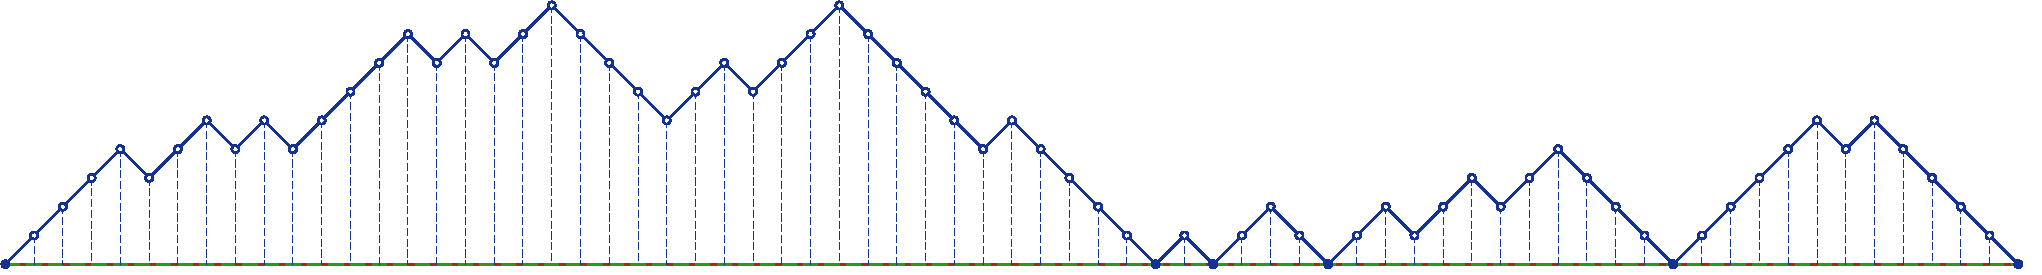
\includegraphics[width=\textwidth]{images/basic_dyck_path.pdf}
    \caption{Simple Dyck path with $n = 35$ up and down steps.}
    \label{fig:basic_dyck}
\end{figure}

Our goal will be to support queries to a uniformly random instance of a Dyck path,
which will in turn allow us to sample other random Catalan objects such as rooted trees, and bracketed expressions.
Specifically, we will want to answer the following queries:
\begin{itemize}
    \item \func{Height}$(i)$: Returns the position of the path after $i$ steps
    \item \func{First-Return}$(i)$: Returns an index $j>i$ such that $\func{Height}(j)=\func{Height}(i)$ and for any $k$ between $i$ and $j$,
    $\func{Height}(k)$ is strictly greater than $\func{Height}(i)$.
\end{itemize}



\subsection{Bijections to other Catalan objects}%
The $\func{Height}$ query is natural for Dyck paths, but the $\func{First-Return}$ query is important in exploring other Catalan objects.
For instance, consider a random well bracketed expression; equivalently an uniform distribution over the Dyck language.
One can construct a trivial bijection between Dyck paths and words in this language
by replacing up and down steps with opening and closing brackets respectively.
The $\func{Height}$ query corresponds to asking for the nesting depth at a certain position in the word,
and $\func{First-Return}(i)$ returns the position of the matching bracket for position $i$.

\label{sec:bijections_to_other_catalan_objects}
\begin{figure}[htbp]
    \centering
    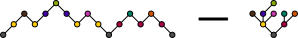
\includegraphics[width=0.9\textwidth]{images/dyck_tree_bijection.pdf}
    \caption{Bijection between Dyck paths and ordered rooted trees.
    For example, successive $\func{First-Return}$ queries on the yellow node would reveal its three children in order from left to right.}
    \label{fig:dyck_tree_bijection}
\end{figure}
There is also a natural bijection between Dyck paths and ordered rooted trees (Figure~\ref{fig:dyck_tree_bijection}),
by considering the Dyck path to be a transcript of a DFS traversal on the tree.
Starting with the root, for each ``up-step'' we move to a new child of the current node, and for each ``down-step'', we backtrack towards the root.
Here, the $\func{Height}$ query returns the depth of a node and the $\func{First-Return}$ query can be used to find the \emph{next child} of a node.
A similar argument shows a bijection to the set of all ordered binary trees.
Moving forwards, we will focus on Dyck paths for the sake of simplicity.



\subsection{Catalan Trapezoids and Generalized Dyck Paths}
In order to sample Dyck paths locally, we will need to analyze more general Catalan objects.
Specifically, we consider a sequence of $U$ up-steps and $D$ down-steps,
such that any prefix of the sequence with $U'$ up and $D'$ down steps satisfies $U'-D' \ge 1-k$.
This means that we start our Dyck path at a height of $k-1$, and we are never allowed to cross below zero (Figure~\ref{fig:complex_dyck}).
\begin{figure}[htbp]
    \centering
    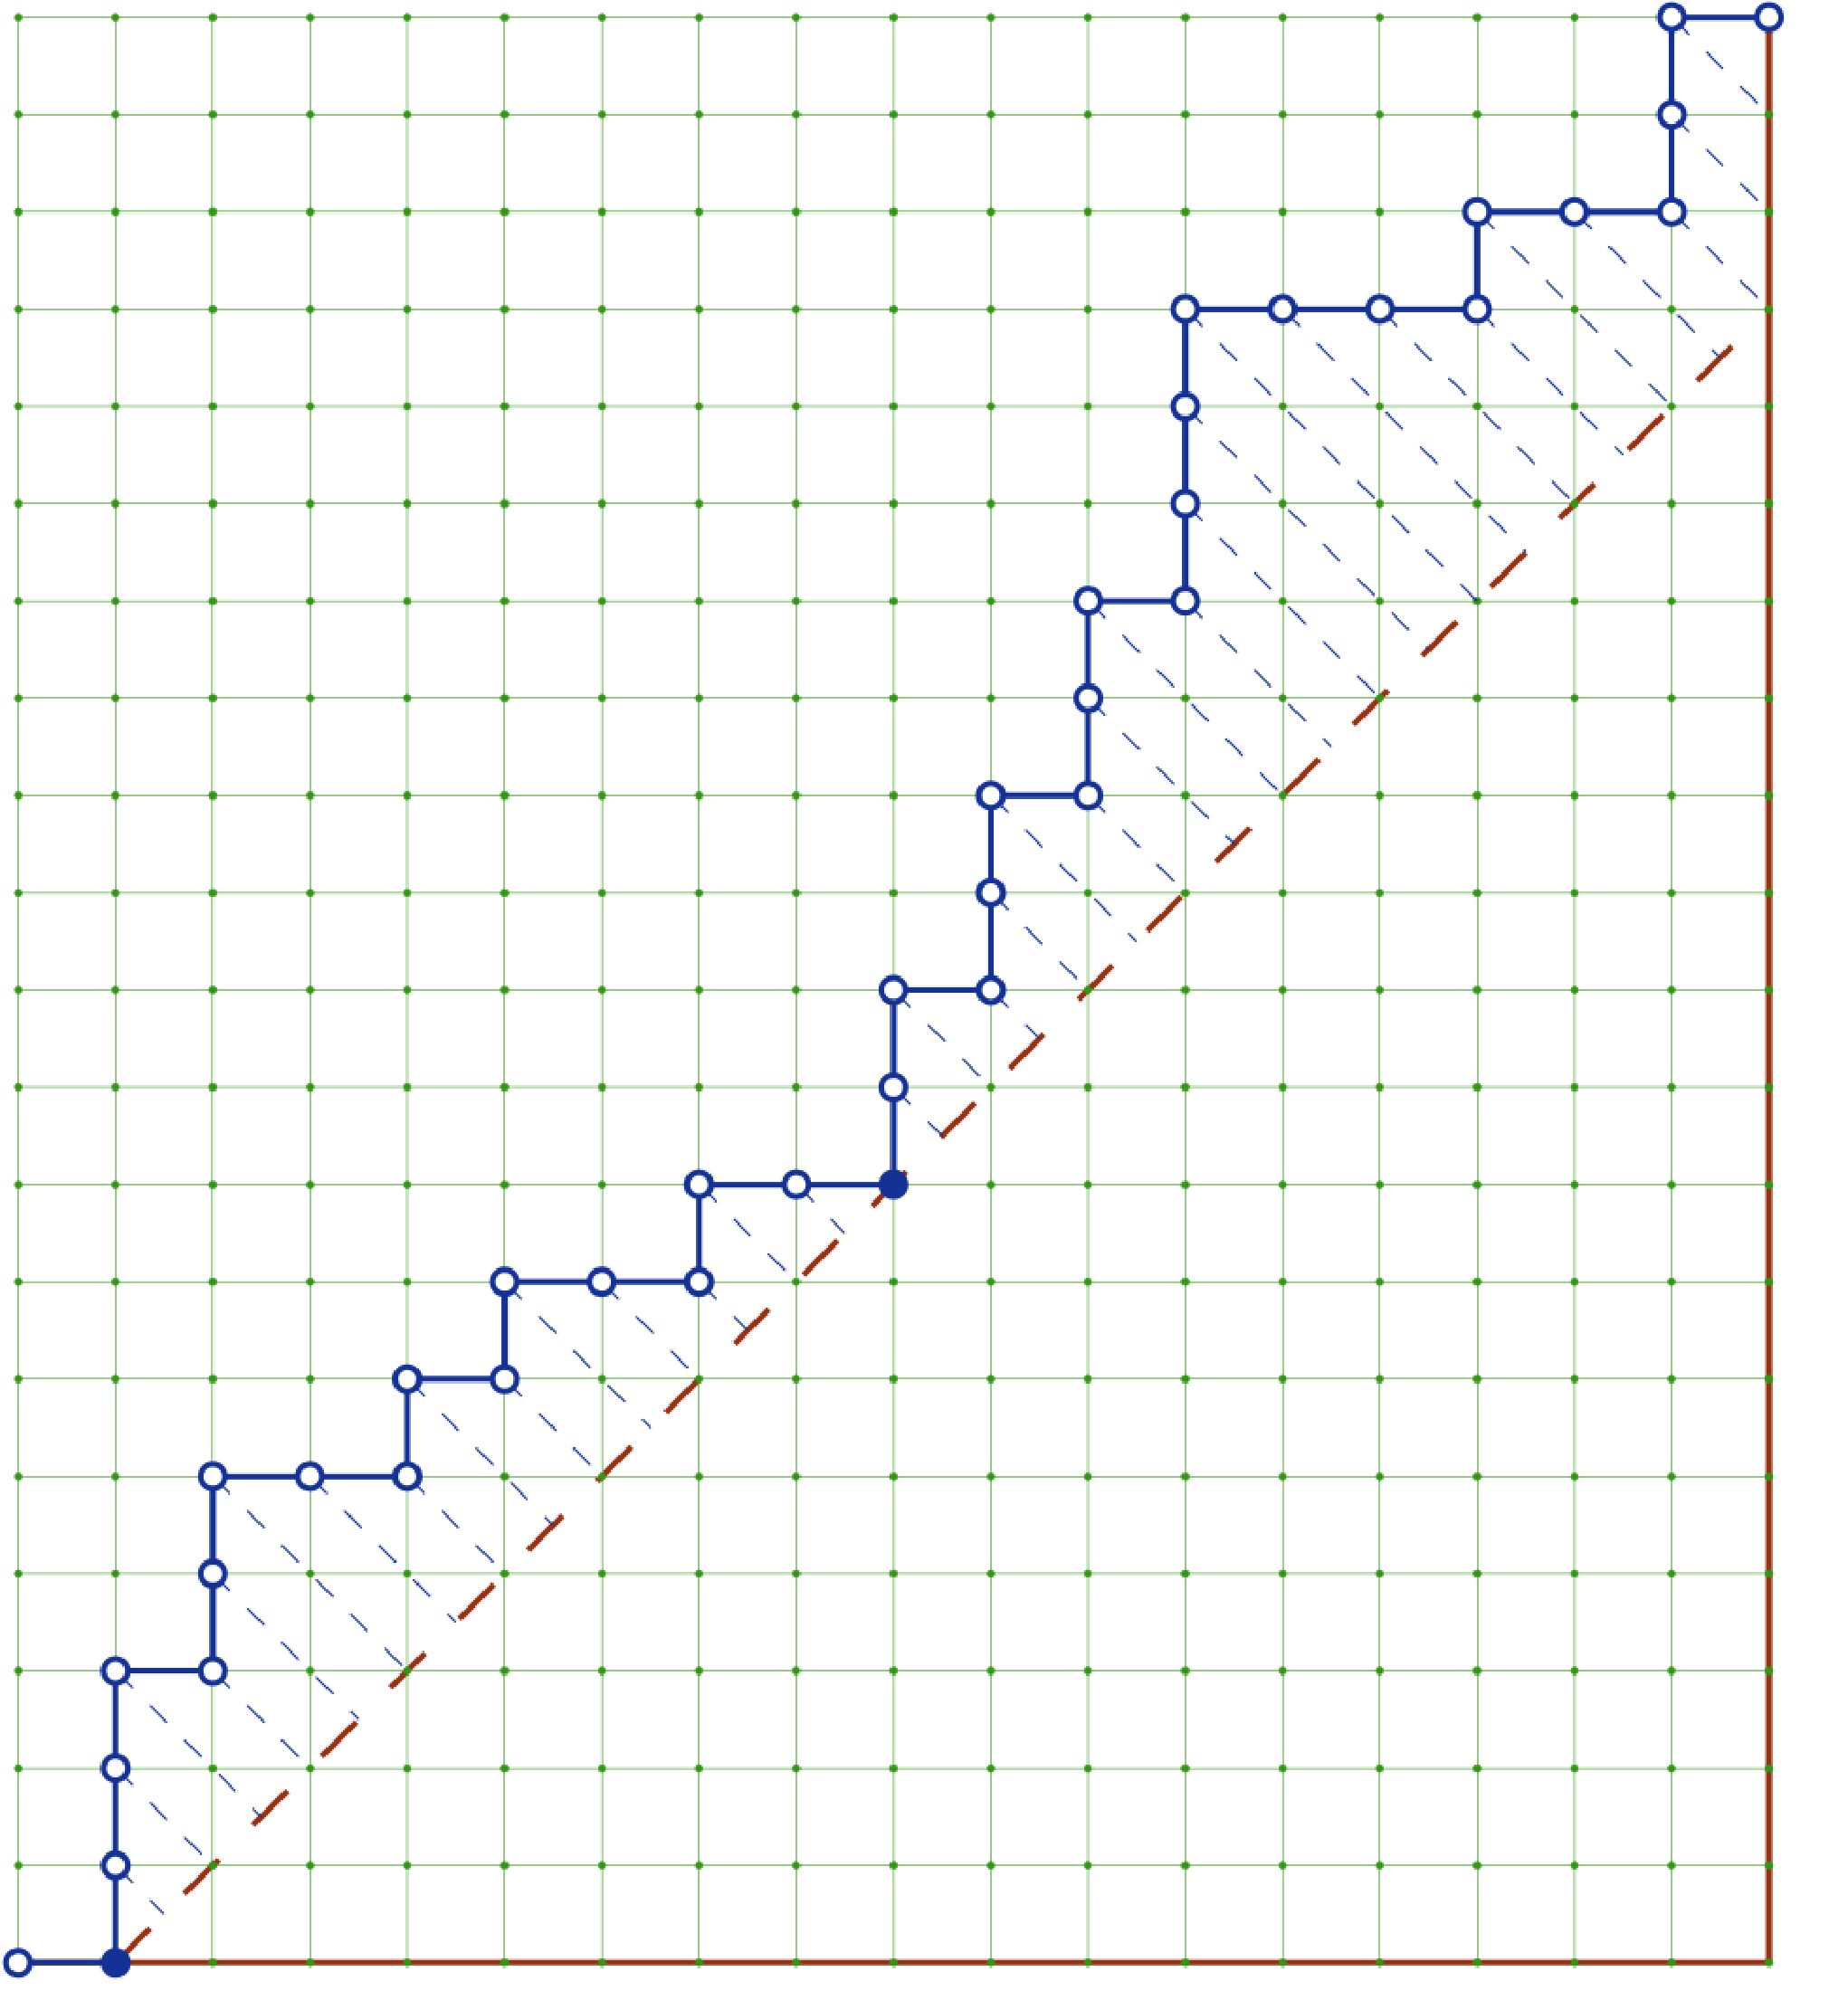
\includegraphics[width=\textwidth]{images/complex_dyck_path.pdf}
    \caption{Generalized Dyck path with $U = 25$, $D = 22$ and $k = 3$.
             Note that the boundary is $k-1 = 2$ units below the starting height.} \label{fig:complex_dyck}
\end{figure}

We will denote the set of such \emph{generalized Dyck paths} as $\mathbb C_k(U,D)$ and the number of paths as $C_k(U,D) = |\mathbb C_k(U,D)|$,
which is an entry in the \textit{Catalan Trapezoid} of order $k$ \cite{trap}.
We also use $\mathsf C_k(U,D)$ to denote the uniform distribution over $\mathbb C_k(n,m)$.
Now, we state a result from \cite{trap} without proof:
\begin{align}
    \label{eq:catalan_trapezoid}
    C_k(U,D)=
    \begin{cases}
    \binom{U+D}{D} &0\le D<k\\
    \binom{U+D}{D} - \binom{U+D}{D-k} &k\le D\le U+k-1\\
    0 &D>U+k-1
    \end{cases}
\end{align}
For $k = 1$ and $n=m$, these represent the vanilla Catalan numbers i.e. $C_n = C_1(n,n)$ (number of simple Dyck paths).
Our goal is to sample from the distribution $\mathsf C_1(n,n)$.

Consider the situation after sampling the height of the Dyck path at various locations $\langle x_1, x_2,\cdots, x_m \rangle$.
The revealed locations partition the path into disjoint \emph{intervals} $[x_i,x_{i+1}]$ where the heights of the endpoints have been sampled.
We define $y_i = \func{Height}(x_i)$ and notice that these intervals are independent of each other.
Specifically, the path in the interval $[x_i, x_{i+1}]$ will be sampled from $\mathsf C_k(U,D)$,
where $k - 1 = y_i$, $U + D = x_{i+1} - x_i$, and $U-D = y_{i+1} - y_i$, and this happens independent of any samples outside the interval.
Next, we will show how one can sample heights within such an interval,
and in Section~\ref{sec:supporting_first_return_queries} we will move on to the more complicated $\func{First-Return}$ queries.

We also maintain a threshold $\mathcal T = \Theta(\log^4 n)$.
If a query lands in an interval that has length less than $\mathcal T$, then we brute force sample the entire interval one step at a time.
Assuming that the probabilities of these events can be approximated efficiently (Lemma~\ref{lem:probability_approximation_oracle},
this take $\poly(\log n)$ time.
\todo{Is this necessary?}



\subsection{Sampling the Height}
\label{sec:sampling_the_height}
We will implement $\func{Height}(t)$ by showing how to (efficiently) sample the position of the path in the midpoint of an existing interval.
We can then extend this to arbitrary positions by running a binary search on the appropriate interval using the midpoint samples.
If the interval in question has odd length, we sample one step on the boundary and proceed with a shortened interval.
\begin{figure}[htpb]
    \centering
    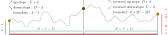
\includegraphics[width=\textwidth]{images/dyck_height_sampling.pdf}
    \caption{The $2B$-interval is split into two equal parts resulting in two separate Dyck problems.
             The green node (center) is the sampled height of the midpoint parameterized by the value of $d$.
             The path considered in both sub-intervals starts at a yellow node (left and right edges) and ends at the green node.
             From this perspective, the path on the right is reversed with up and down steps being swapped.
             A possible path is shown in gray.}
    \label{fig:dyck_height_sampling}
\end{figure}

Our general recursive step is as follows.
We consider an interval of length $2B$ comprising of $2U$ up-steps and $2D$ down-steps where the sum of any prefix cannot be less than $k-1$
i.e. this interval should be sampled from $\mathsf C_k(2U,2D)$ (the factors of two makes the analysis cleaner).
Without loss of generality, we assume that $2D\le B$; if this were not the case, we could simply flip the sequence and negate the elements.
This essentially means that the overall path in the interval is non-decreasing in height.

We will sample the height of the path $B = U+D$ steps into the interval at the midpoint (see Figure~\ref{fig:dyck_height_sampling}).
This is equivalent to sampling the number of up or down steps that get assigned to the first half of the interval.
We parameterize the possibilities by $d$ and define $p_d$ to be the probability that exactly $U+d$ up-steps and $D-d$ down steps
get assigned to the first half, and therefore the second half gets exactly $U-d$ up steps and $D+d$ down steps.
\[
p_d = \frac{S_{left}(d)\cdot S_{right}(d)}{S_{total}(d)}
\]
Here, $S_{left}(d)$ denotes the number of possible paths in the first half (using $U+d$ up steps)
and $S_{right}(d)$ denotes the number of possible paths in the second half (using $U-d$ up steps).
Note that all of these paths have to respect the $k$-boundary constraint (cannot dip more than $k-1$ units below the starting height).
Moving forwards, we will drop the $d$ when referring to the path counts.
We (conceptually) flip the second half of the interval,
such that the corresponding path begins from the end of the $2B$-interval and terminates at the midpoint (Figure~\ref{fig:dyck_height_sampling}).
This results in a different starting point, and the boundary constraint will also be different.
Hence, we define $k' = k + 2U - 2D$  to represent the new boundary constraint (since the final height of the $2B$-interval is $k'-1$).
Finally, $S_{total}$ is the total number of possible paths in the interval (of length $2B$).

We will use the rejection sampling lemma (Lemma~\ref{lem:rejection_sampling} from \cite{huge}.
An important point to note is that in order to apply this lemma, we must be able to compute the $p_d$ values at least approximately.
For now, we will assume that we have access to an oracle that will compute the value for us.
Lemma~\ref{lem:probability_approximation_oracle} shows how to construct such an oracle.
We also use the following lemma to bound the deviation of the path.
\begin{restatable}{lemma}{DyckPathDeviationBound}
\label{lem:DyckPathDeviationBound}
Consider a contiguous \emph{sub-path} of a simple Dyck path of length $2n$
where the sub-path is of length $2B$ comprising of $U$ up-steps and $D$ down-steps (with $U + D = 2B$).
Then there exists a constant $c$ such that the quantities $|B-U|$, $|B-D|$, and $|U-D|$
are all $<c\sqrt{B\log n}$ with probability at least $1-1/n^2$ for every possible sub-path.
\end{restatable}


\subsubsection{The Simple Case: Far Boundary}%
\label{sec:the_simple_case}
\begin{restatable}{lemma}{DyckPathIrrelevantBoundary}
\label{lem:dyck_path_irrelevant_boundary}
Given a Dyck path sampling problem of length $B$ with $U$ up and $D$ down steps with a bounary at $k$,
there exists a constant $c$ such that if $k > c \sqrt{B\log n}$, then the distribution of paths sampled without a boundary $\mathsf C_{\infty}(U,D)$
(hypergeometric sampling) is statistically $\mathcal O(1/n^2)$-close in $L_1$ distance to the distribution of Dyck paths $\mathsf C_k(U+D)$.
\end{restatable}
By Lemma~\ref{lem:dyck_path_irrelevant_boundary}, the problem of sampling from $C_k(2U,2D)$
reduces to sampling from the hypergeometric distribution $C_{\infty}(2U,2D)$ when $k>\mathcal{O}(\sqrt{B\log n})$
i.e. the probabilities $p_d$ can be approximated by:
\[
q_d = \frac{{{B}\choose{D-d}}\cdot{{B}\choose{D+d}}}{{{2B}\choose{2D}}}
\]
This problem of sampling from the hypergeometric distribution is equivalent to the interval summable functions
implemented in \cite{huge} (using $\mathcal O(poly(\log n))$ resources).

\subsubsection{Path Segments Close to Zero}
\label{sec:path_segments_close_to_zero}
A difficult case is when $k = \mathcal{O}(\sqrt{B\log n})$ and we need to compute the actual probability $p_d$,
For the definitions in Section~\ref{sec:sampling_the_height}, we see that:
\begin{align}
    S_{left} = C_k(U+d,D-d)
    &&S_{right} = C_{k'}(U-d,D+d)
    &&S_{total} = C_k(2U,2D)
\end{align}
Here, $k' = k+2U-2D$, and so $k' = \Bo(\sqrt{B\log n})$ (using Lemma~\ref{lem:DyckPathDeviationBound}).
The distribution $\mathsf C_k(2U,2D)$ we wish to sample from has probabilties $p_d = S_{left}\cdot S_{right}/S_{total}$.
We will use rejection sampling (Lemma~\ref{lem:rejection_sampling}) by constructing a different distribution $q_d$
that approximates $p_d$ up to logarithmic factors over the vast majority of its support
(we ignore all $|d|>\Theta(\sqrt{B\log n})$ since the associated probability mass is negligible by Lemma~\ref{lem:DyckPathDeviationBound}).
To invoke the rejection sampling lemma, we present a method to approximate the probabilities $p_d$ in Lemma~\ref{lem:probability_approximation_oracle}.
The only thing left to do is to find an appropriate $q_d$ that also has an \emph{efficiently computable} $CDF$.
Surprisingly, as in Section~\ref{sec:the_simple_case}, we will be able to use the hypergeometric distribution for $q_d$,
\[
q_d = \frac{{B\choose D-d}\cdot{B\choose D+d}}{{2B\choose 2D}} = \frac{{B\choose D-d}\cdot{B\choose U-d}}{{2B\choose 2D}}
\]
However, the argument for why this $q_d$ is a good approximation to $p_d$ is far less straightforward.

First, we consider the case where $k\cdot k'\le 2U+1$.
In this case, we use loose bounds for $S_{left} < \binom{B}{D-d}$ and $S_{right} < \binom{B}{U-d}$
along with the following lemma (proven in Section~\ref{sec:dyck_appendix}).
\begin{restatable}{lemma}{DTotalFarBoundary}
\label{lem:DTotalFarBoundary}
When $kk' > 2U + 1$, $S_{total} > \frac 12\cdot \binom{2B}{2D}$.
\end{restatable}

Combining the three bounds we obtain $p_d < \frac 12 q_d$.
Intuitively, in this case the Dyck boundary is far away, and therefore the number of possible paths
is only a constant factor away from the number of unconstrained paths (see Section~\ref{sec:the_simple_case}).
The case where the boundaries are closer (i.e. $k\cdot k' \le 2U+1$) is trickier,
since the individual counts need not be close to the corresponding binomial counts.
However, in this case we can still ensure that the sampling probability is within poly-logarithmic factors of the binomial sampling probability.
We use the following lemmas (proven in Section~\ref{sec:dyck_appendix}).

\begin{restatable}{lemma}{DLeftBound}
\label{lem:DLeftBound}
$S_{left} \le c_1 \frac{ k\cdot\sqrt{\log n}}{\sqrt{B}}\cdot{{B}\choose{D-d}}$ for some constant $c_1$.
\end{restatable}

\begin{restatable}{lemma}{DRightBound}
\label{lem:DRightBound}
$S_{right} < c_2 \frac{k'\cdot \sqrt{log n}}{\sqrt{B}}\cdot{{B}\choose{U-d}}$ for some constant $c_2$.
\end{restatable}

\begin{restatable}{lemma}{DTotalNearBoundary}
\label{lem:DTotalNearBoundary}
When $kk' \le 2U + 1$, $S_{total} < c_3 \frac{k\cdot k'}{B}\cdot{{2B}\choose{2D}}$ for some constant $c_3$.
\end{restatable}

We can now put these lemmas together to show that $p_d/q_d \le \Theta(\log n)$ and invoke Lemma~\ref{lem:rejection_sampling} to sample the value of $d$.
This gives us the height of the Dyck path at the midpoint of the two given points.

\begin{theorem}
\label{thm:dyck_midpoint_sampling}
Given two positions $a$ and $b$ (and the associated heights) in a Dyck path of length $2n$
with the guarantee that no position between $a$ and $b$ has been sampled yet,
there is an algorithm that returns the height of the path halfway between $a$ and $b$.
Moreover, this algorithm only uses $\mathcal O(poly(\log n))$ resources.
\end{theorem}
\begin{proof}
If $b-a$ is even, we can set $B = (b-a)/2$.
Otherwise, we first sample a single step from $a$ to $a+1$, and then set $B = (b-a-1)/2$.
Since there are only two possibilities for a single step, we can explicitly approximate the probabilities, and then sample accordingly.
This allows us to apply the rejection sampling from Lemma~\ref{lem:rejection_sampling} using $\{ q_d\}$ to obtain samples from $\{ p_d\}$ as defined above.
%Now, if $B > \Theta(\log^2 n)$ we can simply use the rejection sampling procedure described above
%to obtain a $\mathcal O(poly(\log n))$ algorithm.
%Otherwise, we sample each step induividually.
%Since there are only $2B = \Theta(\log^2 n)$ steps, the sampling is still efficient.
\end{proof}

\begin{theorem}
\label{thm:dyck_height_sampling}
There is an algorithm that provides sample access to a Dyck path of length $2n$,
by answering queries of the form \func{Height}$(x)$ with the correctly sampled height of the Dyck path at position $x$
using only $\mathcal O(poly(\log n))$ resources per query.
\end{theorem}
\begin{proof}
The algorithm maintains a successor-predecessor data structure (e.g. Van Emde Boas tree) to store all positions $x$ that have already been sampled.
Each newly sampled position is added to this structure.
Given a query \func{Height}$(x)$, the algorithm first finds the successor and predecessor (say $a$ and $b$) of $x$ among the alredy queried positions.
This provides us the quarantee required to apply Theorem~\ref{thm:dyck_midpoint_sampling},
which allows us to query the height at the midpoint of $a$ and $b$.
We then binary search by updating either the successor or predecessor of $x$ and repeat until we sample the height of position $x$.
%Once the interval length becomes less than $\Theta(\log^2 n)$,
%we perform the full sampling (as in Theorem~\ref{thm:dyck_midpoint_sampling}) which provides us the height at position $x$.
\end{proof}




\subsection{Supporting ``First Return'' Queries}%
\label{sec:supporting_first_return_queries}

In this section, we show how to implement more complex queries to a Dyck path.
Specifically, we introduce $\func{First-Return}(x)$ to allow the user to query the next time the path returns to \func{Height}$(x)$.
Without loss of generality, we impose a restriction that the step from $x$ to $x+1$ is an up-step.
The utility of this kind of query can be seen through other random Catalan objects.
For instance, if we consider a random well bracketed expression, $\func{First-Return}(x)$ is the position of the bracket matching the $x^{th}$ one.
If we consider a random rooted tree,
$\func{First-Return}$ corresponds to the next child of a vertex (see Section~\ref{sec:bijections_to_other_catalan_objects}).
\todo{What if no first return?}

%We will use the following asymptotic formula for \emph{close-to-central} binomial coefficients
%which will allow us the approximate the probabilities in Section~\ref{sec:estimating_the_cdf}.
%\begin{restatable}{lemma}{CentralBinomialCoefficients}
%\label{lem:CentralBinomialCoefficients}
%(From \cite{asymptopia}) If $k = \frac{n \pm c\sqrt n}{2}$ where $c = o(n^{1/6})$,
%we can approximate $\binom{n}{k}$ up to constant factors by the expression $\frac{2^n}{\sqrt n}\cdot \mathlarger e^{-c^2/2}$.
%\end{restatable}

%Recall that we maintain a threshold $\mathcal T = \Theta(\log^4 n)$ such that
%if an un-sampled interval in the Dyck path has length less than $\mathcal T$, then we sample the entire interval using brute force.
%By setting $\mathcal T = \Theta(\log^4 n)$, we see that for intervals with length $B > \mathcal T$,
%the maximum deviations are bounded by $\mathcal O(\sqrt{B\log n}) = \mathcal O(\log^{2.5}n)$ with high probability.
%This means that if we write the deviation as $c\sqrt B$, we see that $c = \mathcal O(\sqrt{\log n})$ which is $o(B^{1/6})$,
%thus satisfying the condition of Lemma~\ref{lem:CentralBinomialCoefficients}.
%\todo{Is this necessary?}


\subsubsection{Maintaining a Boundary Invariant}
\label{sec:maintaining_a_boundary_invariant}
Notice that over a sequence of $\func{Height}$ queries $\langle x_1, x_2,\cdots, x_m \rangle$ to the Dyck path,
many different positions are revealed (possibly in adverserial locations).
This partitions the path into at most $m+1$ disjoint and independent \emph{intervals} with set boundary conditions.
The first step towards finding the $\func{First-Return}$ from position $t$ would be to locate the \emph{interval} where the return occurs.
Even if we had an efficient technique to filter intervals, we would want to avoid considering all $\Theta(m)$ intervals to find the correct one.
In addition, the fact that a specific interval \emph{does not} contain the first return implies dependencies for all subsequent samples.

We resolve these difficulties by maintaining the following invariant.
Consider all positions whose heights have have already been sampled, either directly as a result of user given $\func{Height}$ queries,
or indirectly due to recursive $\func{Height}$ calls; $\langle x_1, x_2,\cdots, x_m \rangle$ (in increasing order i.e. $x_i<x_{i+1}$)
along with their corresponding heights $ \langle y_1, y_2,\cdots, y_m \rangle$.
\begin{invariant}
\label{inv:boundary_invariant}
For any interval $[x_i,x_{i+1}]$ where the heights  of the endpoints have been sampled to be $y_i$ and $y_{i+1}$,
and no other position in the interval has yet been sampled,
the section of the Dyck path between positions $x_i$ and $x_{i+1}$ is constrained to lie above $min(y_i, y_{i+1})$.
\end{invariant}
\begin{figure}[htpb]
    \centering
    \includegraphics[width=\textwidth]{images/dyck_boundary_invariant.pdf}
    \caption{The set of intervals formed by a set of height samples.
        Each interval also has its own boundary constraint (red).
        Invariant~\ref{inv:boundary_invariant} implies that each boundary must coincide with one of the interval endpoints.
        Note that the only interval which does not satisfy this is the third last one (shown in yellow box).}
    \label{fig:dyck_boundary_invariant}
\end{figure}

How can one maintain such an invariant?
After sampling the height of a particular position $x_i$ as $y_i$ (with $x_{i-1} < x_i < x_{i+1}$),
the invariant is potentially broken on either side of $x_i$.
We re-establish the invariant by sampling an additional point on either side.
This proceeds as follows for the interval between $x_i$ and $x_{i+1}$
(see error in Figure~\ref{fig:dyck_boundary_invariant}):
\begin{enumerate}
    \item Sample the lowest height $h$ achieved by the walk between $x_i$ and $x_{i+1}$.
    \item Sample a position $x$ such that $x_i < x < x_{i+1}$ and $\func{Height}(x) = h$.
\end{enumerate}
Since $h$ is the minimum height along this interval, sampling the point $x$ suffices to preserve the invariant.
Lemma~\ref{lem:first_return_interval} shows/how this invariant can be used to efficiently find the interval containing the first return.


\subsubsection{Sampling the Lowest Achievable Height: Mandatory Boundary}
\label{sec:sampling_the_lowest_achievable_height}
First, we need to sample the lowest height $h$ of the walk between $x_i$ and $x_{i+1}$ (with corresponding heights $y_i$ and $y_{i+1}$.
We will also refer to $h$ as the \emph{``mandatory boundary''} in this interval;
i.e. no height in the interval may be lower than the boundary, but at least one point \emph{must} touch the boundary (have height $h$).
We assume that $y_i\le y_{i+1}$ without loss of generality; if this is not the case, swap $x_i$ and $x_{i+1}$ and consider the reversed path.
Say this interval defines a generalized Dyck problem with $U$ up steps and $D$ down steps with a boundary that is $k-1$ units below $y_i$.
\begin{wrapfigure}[16]{R}{0.496\textwidth}
\vspace{-3.0em}
\begin{framed}
    \renewcommand\figurename{Algorithm}
    \caption{Finding the Mandatory boundary}
    \label{alg:mandatory_boundary}
    \begin{algorithmic}[1]
        \Function{Mandatory-Boundary}{$U, D, k$}
            \State {$k_{low}\gets k$}
            \State {$k_{up}\gets 0$}
            \While {$k_{low} < k_{up} - 1$}
                \vspace{.3em}
                \State {$k_{mid}\gets \floor{\frac{(k_{low} + k_{up})}{2}}$}
                \vspace{.3em}
                \State {$P_{total}\gets C_{k_{low}}(U,D) - C_{k_{up}}(U,D)$}
                \vspace{.3em}
                \State {$P_{k_{low}}^{k_{mid}}\gets C_{k_{low}}(U,D) - C_{k_{mid}}(U,D)$}
                \vspace{.3em}
                \State {\textbf{with probability} $P_{k_{low}}^{k_{mid}}/P_{total}$}
                    \State {\hspace{\algorithmicindent}$k_{up}\gets k_{mid}$}
                \State {\textbf{else}}
                    \State {\hspace{\algorithmicindent}$k_{low}\gets k_{mid}$}
            \EndWhile
            \State \Return $k_{low}$
        \EndFunction
    \end{algorithmic}
\end{framed}
\end{wrapfigure}

Given any two boundaries $k_{lower}$ and $k_{upper}$ on this interval (with $k_{lower} < k_{upper}$),
we can count the number of possible generalized Dyck paths that violate the $k_{upper}$ boundary but \emph{not} the $k_{lower}$ boundary as:
\[
P_{k_{lower}}^{k_{upper}} = C_{k_{lower}}(U,D) - C_{k_{upper}}(U,D)
\]
We define the current lower and upper boundaries as $k_{low} = k, k_{up} = 0$, and set $k_{mid} = (k_{low} + k_{up})/2$.
Since we can compute the quantities $P_{k_{mid}}^{k_{up}}$, $P_{k_{low}}^{k_{mid}}$, and $P_{total} = P_{k_{low}}^{k_{up}}$,
we can sample a single bit to decide if the \emph{``lower boundary''} should move up or if the \emph{``upper boundary''} should move down.
We then repeat this binary search until we find $k' = k_{low} = k_{up}-1$ and $k'$ becomes the \emph{``mandatory boundary''}
(i.e. the walk reaches the height exactly $k'-1$ units below $y_i$ but no lower.



\subsubsection{Sampling First Position that Touches the \emph{``Mandatory Boundary''}}
\label{sec:sampling_first_position_touching_mandatory_boundary}

Now that we have a ``\emph{mandatory boundary}'' $k$, we just need to sample a position $x$ with height $h = x_i-k+1$.
In fact, we will do something stronger by sampling the \emph{first} time the walk touches the boundary after $x_i$.
As before, we assume that this interval contains $U$ up steps and $D$ down steps.
\begin{figure}[htpb]
    \centering
    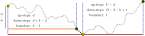
\includegraphics[width=\textwidth]{images/dyck_first_approach_sampling.pdf}
    \caption{Zooming into the error in Figure~\ref{fig:dyck_boundary_invariant}.
        We sample a position $x$ (yellow) on the boundary (red),
        such that the section of the path to the left of $x$ never approaches the red boundary (it respects the orange boundary).}
    \label{fig:dyck_mandatory_boundary_sampling}
\end{figure}

We will parameterize the position $x$ the number of up-steps $d$ between $x_i$ and $x$ (See Figure~\ref{fig:dyck_mandatory_boundary_sampling}).
implying that $x = x_{i} + 2d + k - 1$.
Given a specific $d$, we want to compute the number of valid paths that result in
$d$ up-steps before the first approach to the boundary.
We will calculate this quantity by counting the total number of paths to the left and right
of the first approach and multiplying them together.

As in Section~\ref{sec:path_segments_close_to_zero}, we define
$S_{left}$ to be the number of paths in the sub-interval before the first approach (left side of Figure~\ref{fig:dyck_mandatory_boundary_sampling}),
$S_{right}$ to be the number of paths following the first approach,
and $S_{total}$ to be the total number of paths that touch the ``mandatory boundary'' at $k$
(note that these quantities are functions of $U,D,k$ and $d$, but we drop the parameters for the sake of clarity):
{\small
\begin{align*}
    S_{left} = C_{k}(d, d+k-2)
    &&S_{right} = C_1(U-d, D-d-k+1)
    &&S_{total} = C_k(U,D) - C_{k-1}(U,D)
\end{align*}}
Our goal is to sample $d$ from the distribution $\{ p_d\}$ where $p_d = S_{left}\cdot S_{right}/S_{total}$.
The application of Lemma~\ref{lem:rejection_sampling} requires us to approximate $\{p_d\}$
with a ``well behaved'' $\{q_d\}$ (one whose CDF can be efficiently estimated).
Since we only require a asymptotic (up to $\poly(\log n)$ factors) approximation to $\{p_d\}$,
it suffices to estimate the number of paths asymptotically as well.
Using Equation~\ref{eq:catalan_trapezoid}, we obtain the following approximations for $S_{left}$ and $S_{right}$
(proofs in Section~\ref{sec:omitted_supporting_first_return_queries}).
\begin{restatable}{lemma}{ReturnDLeftBound}
\label{lem:ReturnDLeftBound}
If $d > \log^4 n$, then $S_{left}(d)
= \Theta\left( \frac{2^{2d+k}}{\sqrt{d}}\mathlarger e^{-r_{left}(d)}\cdot \frac{k-1}{d+k-1}\right)$
where $r_{left}(d) = \frac{(k-2)^2}{2(2d+k-2)}$.
Furthermore, $r_{left}(d)=\mathcal O(\log^2 n)$.
\end{restatable}

\begin{restatable}{lemma}{ReturnDRightBound}
\label{lem:ReturnDRightBound}
If $U+D-2d-k > \log^4 n$, then $S_{right}(d)
= \Theta\left( \frac{2^{U+D-2d-k}}{\sqrt{U+d-2d-k}}\mathlarger e^{-r_{right}(d)}\cdot \frac{U-D+k}{U-d+1}\right)$
where $r_{right}(d) = \frac{(U-D-k-1)^2}{4(U+D-2d-k+1)}$.
Furthermore, $r_{right}(d)=\mathcal O(\log^2 n)$.
\end{restatable}

We now consider the values of $d$ that are outside the range of the two preceding lemmas.
These values are the ones where $d < \log^4 n$ or $2d > U+D-k-\log^4 n$.
Since $d$ is the number of up steps in the left sub-interval, $d \ge 0$
and since the length of the right sub-interval nust be non-negative (see Figure~\ref{fig:dyck_mandatory_boundary_sampling}), we get $U+D-2d-k+1 \ge 0$.
Thus, we define the set
\begin{align}
\label{eq:SetDefinition}
    \mathcal R = \left\{ d\ \mathlarger|\ 0\le d < \log^4 n \textrm{\textbf{\ or\ }} -1 < 2d-U-D+k < \log^4 n \right\}
\end{align}
Clearly, we can bound the size of this set as $|\mathcal R| = \mathcal O(\log^4 n)$.
An immediate consequence of Lemma~\ref{lem:ReturnDLeftBound} and Lemma~\ref{lem:ReturnDRightBound} is the following.

\begin{restatable}{corollary}{ReturnProbabilityBoundNotNormalized}
\label{cor:ReturnProbabilityBoundNotNormalized}
When $d\not \in \mathcal R$,
$S_{left}(d)\cdot S_{right}(d)
= \Theta\left( \frac{2^{U+D}}{\sqrt{d(U+D-2d-k)}}\cdot \mathlarger e^{-r(d)} \cdot \frac{k-1}{d+k-1}\cdot\frac{U-D+k}{U-d+1}\right)$
where $r(d)=\mathcal O(\log^2 n)$.
\end{restatable}



\subsubsection{Estimating the CDF}
\label{sec:estimating_the_cdf}
We use these observations to construct a suitable $\{ q_d\}$ that can be used to invoke the rejection sampling lemma.
This is achieved by constructing a piecewise continuous function $\hat q$, such that $\hat q(\delta)$ approximates $p_{\floor\delta}$,
and then using the integral of $\hat q$ to define $q_d$.
%In addition to being a good approximation to $\{ p_d\}$, $\{ q_d\}$ must be of a form that allows us to compute its CDF efficiently.
First, we rewrite $p_d = \Theta\left(\mathcal K \cdot f(d)\cdot e^{-r(d)}\right)$ where:
{\small
    \begin{align}
    \label{eq:dyck_integrable_function}
        \mathcal K = \frac{2^{U+D}}{S_{total}} = \frac{2^{U+D}}{C_k(U,D)-C_{k-1}(U,D)}\ \ \ \
        &&f(d) = \frac{(k-1)(U-D+k)}{\sqrt{d(U+D-2d-k)}(d+k-1)(U-d+1)}
    \end{align}}
Notice that $\mathcal K$ is a constant and $f(d)$ is a function whose integral has a closed form.
Using the fact that $r(d) = \mathcal O(\log^2 n)$ (from Corollary~\ref{cor:ReturnProbabilityBoundNotNormalized}), we obtain the following lemma:

\begin{lemma}
\label{lem:ReturnProbabilityPiecewiseContinuous}
Given the piecewise continuous function
\begin{align*}
    \hat q(\delta) &=
    \begin{cases}
        p_{\floor\delta} &\mbox{if } \floor\delta \in \mathcal R \\ 
        \mathcal K\cdot f(\delta)\cdot exp\left(-\lfloor{r({\scriptstyle\floor\delta})}\rfloor\right)
        & \mbox{if } \floor\delta \not\in \mathcal R
    \end{cases}
    && \mathlarger \implies
    && p_d = \Theta\left( \int\limits_d^{d+1} \hat q(\delta)\right)
\end{align*}
Furthermore, $\hat q(\delta)$ has $\mathcal O(\log^4 n)$ continuous pieces.
%Note that this integral has a closed form for a fixed value of $\floor{r(d)}$.
\end{lemma}
\begin{proof}
For $d \in \mathcal R$, the integral trivially evaluates to exactly $p_d$.
For $d\not\in \mathcal R$, it suffices to show that $p_d = \Theta\left( \hat q(\delta)\right)$ for all $\delta\in [d,d+1)$.
We already know that $p_d = \Theta\left( \mathcal K\cdot f(d)\cdot e^{-r(d)}\right)$.
Moreover, for any $\delta\in [d,d+1)$, the exponential term $e^{-\floor{r(\floor\delta)}}$ in $\hat q(\delta)$ is within a factor of $e$ of the original $e^{-r(d)}$ term.

For all $\mathcal O(\log^4 n)$ values $d\in \mathcal R$, $\hat q(\delta)$ is constant on the interval $[d,d+1]$.
Since $r(d) = \mathcal O(\log^2 n)$ by Corollary~\ref{cor:ReturnProbabilityBoundNotNormalized},
the exponential term $e^{-\floor{r(\floor\delta)}}$ in $\hat q(\delta)$ taken on at most $\mathcal O(\log^2 n)$ values.
Thus, $\hat q$ is continuous for a range of $\delta$ correspoding to a fixed value of $\floor{r(\floor\delta)}$,
and so, we conclude that $\hat q$ is piecewise continuous with $\mathcal O(\log n)$ pieces.
so, we conclude that $\hat q$ is piecewise continuous with $\mathcal O(\log n)$ pieces.
\end{proof}

Now, we have everything in place to define the distribution $\{ q_d\}$ that we will be sampling from.
Specifically, we will define $q_d$ and it's CDF $Q_d$ as follows ($\mathcal N$ is the normalizing factor):
{\small
    \begin{align}
        q_d = \left(\int\limits_d^{d+1} \hat q(\delta)\right)\cdot \frac{1}{\mathcal N}
        && Q_d = \left(\int\limits_0^{d+1} \hat q(\delta)\right)\cdot \frac{1}{\mathcal N}
        && \textrm{where }\ \mathcal N = \int\limits_0^{d_{max}+1} \hat q(\delta)
    \end{align}}
%Here the normalizing factor $\mathcal N$ is $\int_0^{d_{max}+1} \hat q(\delta)$.
To show that these can be computed efficiently, it suffices to show that any integral of $\hat q(\delta)$ can be efficiently evaluated.
This follows from the fact that $\hat q$ is piecewise continuous with $\mathcal O(\log^4)$ pieces (Lemma~\ref{lem:ReturnProbabilityPiecewiseContinuous}),
each of which has a closed form integral (since $f(d)$ defined in Equation~\ref{eq:dyck_integrable_function} has an integral), thus yielding:
\begin{lemma}
\label{lem:ReturnProbabilityPiecewiseContinuousIntegral}
Given the function $\hat q_d$ defined in Lemma~\ref{lem:ReturnProbabilityPiecewiseContinuous},
it is possible to compute the integral $\int_{d_1}^{d_2+1} \hat q(\delta)$ in $\poly(\log n)$ time for any valid $d_1, d_2\in \mathbb Z$
(the bounds must be such that $d_i \ge 0$ and $U+D-2d_i-k+1 \ge 0$).
\end{lemma}

Now, we are finally ready to use Lemma~\ref{lem:rejection_sampling} to sample $d$ from the distribution $\{p_d\}$,
using the efficient sampling procedure for $\{q_d\}$.
The only other requirement is the ability to approximate the $p_d$ values, which follows from Lemma~\ref{lem:probability_approximation_oracle}.
\begin{theorem}
\label{thm:first_return_in_interval}
Given a sub-interval $[x_{i},x_{i+1}]$ of a random Dyck path of length $2n$,
such that the only sampled heights in the interval are $y_i=\func{Height}(x_i)$ and $y_{i+1}=\func{Height}(x_{i+1})$,
and a mandatory boundary constraint at $k$,
there exists an algorithm that samples a point $x$ within the interval such that $\func{Height}(x) = y_i-k+1$,
using $\poly(\log n)$ time, random bits, and additional space.
\end{theorem}



\subsubsection{Finding the Correct Interval: $\func{First-Return}$ Query}
As before, consider all positions that have been queried already $ \langle x_1, x_2,\cdots, x_m \rangle$ (in increasing order)
along with their corresponding heights $ \langle y_1, y_2,\cdots, y_m \rangle$.
\begin{restatable}{lemma}{FirstReturnInterval}
\label{lem:first_return_interval}
For any position $x_i$, assuming that Invariant~\ref{inv:boundary_invariant} holds,
we can find the interval $(x_{k-1},x_{k}]$ that contains $\func{First-Return}(x_i)$
We do this by by setting $k$ to be either the smallest index $f>i$ such that $y_f\le y_i$ or setting $k=i+1$.
\end{restatable}
\begin{proof}
We assume the contrary i.e. there exists some $k\not=f$ and $k\not=i+1$ such that the correct interval is $(x_{k-1},x_k]$.
Since $y_f<y_i$, the position of first return to $y_i$ happens in the range $(x_i,x_f]$.
So, the only possibility is $i+1 < k \le f-1$.
By the definition of $y_f$, we know that both $y_k$ and $y_{k-1}$ are strictly larger than $y_i$.
Invariant~\ref{inv:boundary_invariant} implies that the boundary for this interval $(y_{k-1},y_k]$ is at $\min(y_{k-1},y_k) > y_i$.
So, it is not possible for the first return to be in this interval.
\end{proof}

The good news is that there are only two intervals that we need to worry about.
Now, the challenge is to find the smallest index $f>i$ such that $y_f\le y_i$.
To this end, we define $M_{[a,b]}$ as the minimum sampled height in the range of positions $[a,b]$.
%(lowest $y$-value) of any sampled boundary in the range of positions $[a,b]$ along the Dyck path.

One solution is to maintain a range tree $\mathbf R$ \cite{comp_geo} over the range $[2n]$.
Assuming that $2n = 2^l$, we can view $\mathbf R$ as a complete binary tree with depth $r$.
Every non-leaf node is denoted by $\mathbf R_{[a,b]}$, and corresponds to a range $[a,b]\subseteq[2n]$ that is the union of the ranges of its children.
Each $\mathbf R_{[a,b]}$ stores the value $M_{[a,b]}$ which is is the minimum sampled height
in the range of positions $[a,b]$, or $\infty$ if none of the heights have been revealed.
%the height of the last boundary update that affected the entire range $[a,b]$.
The leaf nodes are denoted as $\{\mathbf R_i\}_{i\in[2n]}$, and correspond to the singleton range corresponding to position $i\in [2n]$.
%and by definition, this is the min of the values stored at the children of $\mathbf R_{[a,b]}$.
Note that a node at depth $l'$ will correspond to a range of size $2^{l-l'}$, with the root being associated with the entire range $[2n]$.

We say that the range $[a,b]$ is \emph{canonical} if it corresponds to a range of some $\mathbf{R}_{[a,b]}$ in $\mathbf R$.
By the property of range trees, any arbitrary range can be decomposed into a disjoint union of $O(\log n)$ canonical ranges.
We implement $\mathbf{R}$ to support the following operations:
\begin{itemize}
    \item \func{Update}$(x,y)$: Update the height of the position $x$ to $y$.\\
    This update affects all ranges $[a_i,b_i]$ containing $x$.
    So, for each $[a_i,b_i]$ we set $M_{[a_i,b_i]} = \min\left( M_{[a_i,b_i]}, y\right)$.
    \item \func{Query}$(a,b)$: Return the minimum boundary height in the range $[a,b]$.\\
    We decompose $[a,b]$ into $\mathcal O(\log n)$ \emph{canonical} ranges $ \langle r_1, r_2,\cdots\rangle$,
    %For each $r_i$, we compute $M_{r_i}$ as the minimum over all $R_r$ such that the \emph{canonical} range $r$ contains $r_i$.
    %Equivalently, we set $M_{r_i}$ to be the minimum of all values on the path from $\mathbf R_{r_i}$ to the root of $\mathbf R$,
    %which takes $\mathcal O(\log n)$ time.
    %Note that the values stores in the sub-tree rooted at $\mathbf R_{r_i}$ do not affect $M_{r_i}$,
    %since the coreesponding boundary updates did not affect the \emph{entire} range $r_i$ (these updates only affected canonical sub-ranges of $r_i$).
    and return the minimum of all the $M_{r_i}$ values as $M_{[a,b]}$ (since $[a,b]$ is the union of all $r_i$).
\end{itemize}

Now, we can binary search for $f$ by guessing a value $f'$ and checking if $\func{Query}(x_i,x_{f'}) \le y_i$.
Overall, this requires $\mathcal O(\log n)$ calls to $\func{Query}$, each of which makes $\mathcal O(\log n)$ probes to the range tree.
To avoid an initialization overhead, we only create the node $\mathbf{R}_{[a,b]}$ during the first $\func{Update}$ affecting a position $x\in[a,b]$.
Since a call to $\func{Update}$ can create at most $\mathcal O(\log n)$ new nodes in $\mathbf R$,
the additional space required for each $\func{Height}$ or $\func{First-Return}$ query is still bounded.

\begin{theorem}
\label{thm:dyck_first_return_sampling}
There is an algorithm using $\mathcal O(poly(\log n))$ resources per query that provides sample access to a Dyck path of length $2n$
by answering queries of the form \func{First-Return}$(x_i)$ with the correctly sampled position $y$;
where $y>x_i$ is the position where the Dyck path first returns to $\func{Height}(x_i)$ after position $x_i$.
\end{theorem}
\begin{proof}
We first query the interval $(x_i,x_{i+1}]$ to find a first return using Theorem~\ref{thm:first_return_in_interval}.
If a return is not found, we calculate $f$ using the range tree data structure described above.
Since $x_{f-1}<x_i\le x_f$ by definition, the interval $(x_{f-1},x_f]$ must contain a position at height $y_i$.
We sample a point in the middle of this interval and fix the boundary invariant by sampling another point,
essentially breaking it up into $\mathcal O(1)$ sub-intervals each at most half the size of the original.
Based on the new samples, we again find the (newly created) sub-interval containing the first return in $\mathcal O(1)$ time.
We repeat up to $\mathcal O(\log n)$ times, performing binary search to find the position of the first return.
%\todo{Remove Threshold}
%We repeat up to $\mathcal O(\log n)$ times until the current interval size drops below the threshold $\mathcal T$.
%Then we spend $\widetilde{\mathcal O}(\mathcal T)$ time to brute force sample this interval and find the first return position (if it wasn't revealed in previous steps).
\end{proof}

%\subsection{Domino Tiling}
We will consider the problem of tiling a square grid with dominos.
This problem has a long histor and various importtant applications in statistical physics.
Specifically, we will focus on the local generation of domino tilings from the uniform distribution.

\subsection{$2\times n$ Domino Tiling}
The simplest version of the problem is one where we are given a $2\times n$ grid (Figure~\ref{fig:dom2}.
The queries will be as an index, and the generator should report the orientation of the domino at the $i^{th}$ position in the grid.
%\begin{figure}[htbp]
    %\centering
    %\includegraphics[width=\textwidth]{images/domino2.png}
    %\caption{}
    %\label{fig:dom2}
%\end{figure}

It is a well known result \todo{cite} that the number of tilings of a $2\times n$ grid is exactly $F_n$.

To aid with generalization, we will instead allow the generator to respond with the splitting boundary of the current tiling instead.
For example, in Figure~\ref{fig:b20}, the boundary is a vertical line at the specified position.
In Figure~\ref{fig:b21}, the boundary is horizontal, indicating that there are two horizontal dominos at that location.
Note that Figure~\ref{fig:b22} is impossible for a $2\times n$ grid.
It should be clear that this query model is equivalent.

\begin{figure}[h]
    \centering
    \subfloat[][]{
        \includegraphics[width=0.5\linewidth]{images/tile2-0.jpg}
        \label{fig:b20}
    }
    \subfloat[][]{
        \includegraphics[width=0.5\linewidth]{images/tile2-1.jpg}
        \label{fig:b21}
    }

    \subfloat[][]{
        \includegraphics[width=0.5\linewidth]{images/tile2-2.jpg}
        \label{fig:b22}
    }
    \caption{Caption for this figure with two images}
    \label{fig:boundary2}
\end{figure}

Now, consider a query to the location $i$, such that all positions between $i-a$ and $i+b$ have not been queriesd so far.
So, there is a blank $2\times(a+b)$ size sub-grid that we have to sample from.
Let us consider the number of possible tilings resulting from each possible splitting boundary.
\begin{enumerate}
    \item Vertical Boundary -- This indicates that we divide the region into two sub-grids with sizes
          $2\times a$ and $2\times b$.
          So, the total number of possible tilings is exactly $F_a\cdot F_b$.
    \item Horizontal Boundary -- This indicates that we divide the region into two sub-grids with sizes
          $2\times (a-1)$ and $2\times (b-1)$.
          So, the total number of possible tilings is exactly $F_{a-1}\cdot F_{b-1}$.
\end{enumerate}

So the probabilities are computed as $\frac{F_a\cdot F_b}{F_a\cdot F_b + F_{a-1}\cdot F_{b-1}}$
and $\frac{F_{a-1}\cdot F_{b-1}}{F_a\cdot F_b + F_{a-1}\cdot F_{b-1}}$.
Now, we face the issue of approximating these fractions.
If either of the values $a$ or $b$ are less than $\Theta(\sqrt n)$,
then we can compute the exact value of the corresponding $F_a$ or $F_b$.
Otherwise, we use Lemma~\ref{lem:rat_conv} to approximate $F_a=\phi\cdot F_{a-1}$ and $F_b=\phi\cdot F_{b-1}$.
So, the probability of the vertical boundary becomes
$$
\frac{F_a\cdot F_b}{F_a\cdot F_b + F_{a-1}\cdot F_{b-1}} = \frac{\phi^2}{\phi^2+1}
$$
Similarly, the probability of a horizontal split with a top and bottom domino becomes $1/(\phi^2+1)$.
Note that this also determines the two adjacent boundaries.

The only information we needed to make this query was the extent of the un-queried interval $[i-a, i+b]$.
We can use any standard data-structure that allows insertion in positions $\{1, 2\cdots,n+1\}$,
and provides successor and predecessor queries.

Here's we can be fancy and use Van-Emde-Boas trees to get a $\Bo(\log\log n)$ query time.
However, in some cases, the exact value of a Fibonacci number still needs to be computed, and this takes $\Bo(\log n)$ time.
The faster queries only work when the new query is "far enough" ($\Bo(\log n)$ distance) away from all previous queries.


\section{Random Coloring of a Graph}%
\label{sec:random_coloring_of_a_graph}

\todo{Query access}
We wish to locally sample an uniformly random coloring of a graph.
A $q$-coloring of a graph $G = (V, E)$ is a function $\sigma : V\rightarrow [q]$,
such that for all $(u,v)\in E$, $\sigma_u \not= \sigma_v$.
We will consider only bounded degree graphs, i.e. graphs with max degree $\le \Delta$.
Otherwise, the coloring problem becomes NP-hard\todo{cite}.

Using the technique of path-coupling, Vigoda \todo{cite} showed that for $q > 2\Delta$,
one can sample an uniformly random coloring by using a MCMC algorithm.

The Markov Chain proceeds in $T$ steps. The state of the chain at time $t$ is given by $\vec X^t\in [q]^{|V|}$.
Specifically, the color of vertex $v$ at step $t$ is $\vec X^t_v$.

In each step of the Markov process, a pair $(v, c)\in V\times [q]$ is sampled uniformly at random.
Subsequently, if the recoloring of vertex $v$ with color $c$ does not result in a conflict with $v$'s neighbors,
i.e. $c\not\in \left\{ X^t_u : u\in \Gamma(v)\right\}$, then the vertex is recolored i.e. $X_v^{t+1}\leftarrow c$.

After running the MC for $T = \mathcal{O}(n\log n)$ steps we reach the stationary distribution ($\epsilon$ close),
and the coloring is an uniformly random one.

\textbf{Exact Bound:}
$t_{mix}(\epsilon) \le \left( \frac{q-\Delta}{q-2\Delta}\right)n\left( \log n + \log(1/\epsilon)\right)$
\todo{cite book (Peres, Lyons)}



\subsection{Modified Glauber Dynamics}%
\label{sub:modified_glauber_dynamics}

Now we define a modified Markov Chain that proceeds in epochs.
We denote the initial coloring of the graph by $\vec X^0$ and the state of the coloring after the $k^{th}$ epoch by $\vec X^k$.
In the $k^{th}$ epoch $\mathcal E_k$:
\begin{itemize}
    \item Sample $n = |V|$ colors $ \langle c_1, c_2,\cdots, c_n \rangle$ from $[q]$, where $c_v$ is the proposed color for vertex $v$.
    \item For each vertex $v$, we set $\vec X^k_v$ to $c_v$ if for all neighbors $w$ of $v$, $\vec X^k_w\not=c_v$ and $\vec X^{k-1}_w\not=c_v$.
\end{itemize}
%\begin{itemize}
    %\item Pick a random permutation $\pi^{(i)}$ of the vertices $V$.
    %\item Sample $n = |V|$ colors $ \langle c_1, c_2,\cdots, c_n \rangle$ from $[q]$.
    %\item Perform the standard update using the pairs $\left\langle (\pi^{(i)}_1, c_1), (\pi^{(i)}_2, c_2), \cdots, (\pi^{(i)}_n, c_n)\right\rangle$.
%\end{itemize}

This procedure is a special case of the \emph{Local Glauber Dynamics} presented in \cite{mohsen}.
The goal in \cite{mohsen} is to find a simultaneous update rule that causes few conflicts among neighbors (and converges to the correct distribution).
Notice that we can have adjacent nodes update in the same epoch, and this can also be implemented locally using \todo{what?}.
However for the sake of succinctness and because this would only improve a constant factor in the exponent,
we use their update rule and avoid a tedious path coupling argument.
\todo{Wording: a vertex needs to avoid $\le 2\Delta$ colors in order to be  accepted}

\todo{Cite Path Coupling}
For the path coupling argument, we define the standard pre-metric on the space for all possible colorings (not necessarily valid ones).
Given two colorings $X$ and $Y$, we define $d(X,Y)$ as the number of vertices $v$ such that $X_v\not= Y_v$.

We define a coupling $(X,Y)\rightarrow(X',Y')$ where $X$ and $Y$ differ only at a single vertex $v$ such that $X_v = c_X$ and $Y_v = c_Y$.
Now, we pick a random permutation of the vertices along with uniformly sampled colors:
\[
\left\langle (v_1, c_1), (v_2, c_2), \cdots, (v_n, c_n)\right\rangle
= \left\langle (\pi_1, c_1), (\pi_2, c_2), \cdots, (\pi_n, c_n)\right\rangle
\]
Now, for each $(v_i, c_i)$ in order, we update the coloring of $X$ and $Y$ as follows:
\begin{itemize}
    \item If the current color of $v_i$ as well as $c_i$ is in $\{c_X,c_Y\}$,
    then the $X$ chain picks the color $c_i$ and the $Y$ chain picks the other color.
\end{itemize}

\begin{lemma}
\label{lem:mohsen_single_epoch_distance}
If $q = 2\alpha\Delta$ and $d(X, Y) = 1$, then $\mathbb E[d(X',Y')] \le 1-\left( 1-\frac1{2\alpha}\right)e^{-3/\alpha} + \frac{1/2\alpha}{1-1/\alpha}$
\end{lemma}
\begin{corollary}
\label{cor:single_epoch_distansce}
If $q \ge 9\Delta$ and $d(X, Y) = 1$, then $\mathbb E[d(X',Y')] < \frac1{e^{1/3}}$
\end{corollary}

\begin{theorem}
\label{thm:modified_mixing_time}
If $q\ge 9\Delta$, then the Markov Chain is mixed after $\tau_{mix}(\epsilon) = 3\ln n + 3\ln(1/\epsilon)$ epochs.
\end{theorem}
\begin{proof}
\todo{Write proof}
\end{proof}




\subsection{Local Coloring Algorithm}%
\label{sub:local_coloring_algortihm}
Given a vertex $v$, the local-access generator has to output the color of $v$ after running $t \le 2\ln n$ epochs of \emph{Modified Glauber Dynamics}.
We will define the number of colors as $q = \alpha\Delta$ where $\alpha > 1$.

%Each epoch can be implemented a local generator for a permutation of $V$.
%Specifically, each epoch is a sequence of vertex and color samples:
%\[
%\chi^{(i)}
%= \left\langle (v^{(i)}_1, c^{(i)}_1), (v^{(i)}_2, c^{(i)}_2), (v^{(i)}_3, c^{(i)}_3), \cdots, (v^{(i)}_T, c^{(i)}_T)\right\rangle
%\thicksim_{\mathcal U} \left( V\times [q]\right)^T
%\]
%Here, $\left\{ v^{(i)}_1, v^{(i)}_2,\cdots, v^{(i)}_n\right\}$ is a permutation of all the vertices.
%A position $j$ in the sequence is labeled \emph{``ACCEPT''} if at the $j^{th}$ step,
%$v^{(i)}_j$ was recolored to $c^{(i)}_j$ (no conflicts with neighbors).
%Otherwise, position $j$ is marked \emph{``REJECT''}.
%We define $X^{(i)}_v = 1$ if the sample for $v$ in the $i^{th}$ epoch $(v, c^{(i)}_j)$ is accepted and $X^{(i)}_v = 0$ otherwise.

%We also define $\mathcal C^{(i)}_v$ to be the color sampled for vertex $v$ in the $i^{th}$ epoch,
%and $\mathcal I^{(i)}_v$ to be the corresponding index $j$.

Each epoch is a vector of color samples $\vec C^{i} \thicksim_{\mathcal U} [q]^n$.
Note that these values are fully independent and as such any $\vec C^i_v$ can be sampled trivially.
We also use $\vec X^i$ to denote the final vector of vertex colors at the end of the $i^{th}$ epoch.
Finally, we define indicator variables $\bm \chi^i_v$ to denote if the color for vertex $v$ was accepted at the $i^{th}$ epoch;
$\bm \chi^i_v = 1$ if and only if for all neighbors $w\in \Gamma(v)$,
we satisfy the condition $\vec  C^i_v\not= \vec X^{i-1}_w$ and $\vec C^i_v\not= \vec C^i_w$.
So, the color of a vertex $v$ after the $t^{th}$ epoch $\vec X^t_v$ is set to be $\vec C^i_v$
where $i\le t$ is the largest index such that $\bm \chi^i_v=1$.
Algorithm~\ref{alg:coloring} shows the procedure for querying the value of $\vec X^t_v$.

\begin{algorithm}[H]
\caption{Generator}
\begin{algorithmic}[1]

\Procedure{Color}{$v, t$}
    \For{$i \gets [ t, t-1, t-2 \cdots 1 ]$}
        \If {\func{Accepted}($i, v$)}
            \State \Return $C^i_v$
        \EndIf
    \EndFor
\EndProcedure

\Procedure{Accepted}{$v, t$}
    \State {$c\gets C^t_v$}
    \For{$w \gets \Gamma(v)$}
        \State {$flag\gets \ZERO$}
        \For{$t' \gets [t, t-1, t-2, \cdots, 1]$}
            \If {$t' \not= t$ \textbf{or} $\mathcal I^{(t)}_w < \mathcal I^{(t)}_v$}
                \If {$\mathcal C^{(t')}_w = c$ \textbf{and} \func{Accepted}($w, t'$)}
                    \State $flag\gets \ONE$
                    \While{$t' < t$}
                        \State $t'\gets t' + 1$
                        \If {\func{Accepted}($w, t'$)}
                            \State $flag\gets \ZERO$
                            \State \textbf{break}
                        \EndIf
                    \EndWhile
                    \If {$flag = \ONE$}
                        \State \Return $\ZERO$
                    \EndIf
                    \State \textbf{break}
               \EndIf
           \EndIf
        \EndFor
    \EndFor
    \State \Return $\ONE$
\EndProcedure

\end{algorithmic}
\label{alg:coloring}
\end{algorithm}

When the algorithm is asked for the final color of $v$, it finds the last epoch in which $v$ was accepted.
Since there are only $\mathcal O(\log n)$ epochs, we focus our attention on the subroutine $\func{Accepted}$ that samples the value of $\bm\chi^t_v$.
The algorithm iterates through the neighbors $w$ of $v$, and check for conflicts with the proposed color $c=\vec C^t_v$.
The condition $c\not= \vec C^t_w$ is can easily be checked by sampling $\vec C^t_w$ in the current epoch.
If no conflict is seen, the next step is to check whether $c\not= \vec X^{t-1}_w$.

We first iterate through all the epochs in reverse order to check whether the color $c$ was ever proposed for vertex $w$.
If not, we can ignore $w$, and otherwise let's say that the last proposal for $c$ was at epoch $t'$ i.e. $\vec C^{t'}_w = c$.
Now, we need to recursively check if this proposal was $\func{Accepted}$.
If it was, we move to epoch $t'+1$ to see if $w$'s color was replaced.
If not, we check epoch $t'+2$ and so on until we reach epoch $t-1$.
At this point we have seen that $\bm\chi^{t'}_w = 1$ (color $c$ was accepted) and every subsequent proposal until the current epoch was rejected
i.e. $\vec X^{t-1}_w = c$ and this leads to a conflict with $v$'s current proposal for color $c$ and hence $\bm\chi^t_v = 0$.
If at any of the iterations, we see that a different proposal was accepted, then $w$ does not cause a conflict and we can move on to the next neighbor.
If we exhaust all the neighbors and don't find any conflicts then $\bm\chi^t_v = 1$.

\begin{lemma}
\label{lem:color_reject_probability}
The probability that any given proposal is rejected $\mathbb P[\bm\chi^t_v=0]$ is at most $1/\alpha$.
Moreover, this upper bound holds even if we condition on all the values in $\vec C$ except $\vec C^t_v$.
\end{lemma}
\begin{proof}
A rejection can occur due to a conflict with at most $2\Delta$ possible values in $\{ C^t_w, X^{t-1}_w | w\in\Gamma(v)\}$.
Since there are $2\alpha\Delta$ colors, the rejection probability is at most $1/\alpha$.
\end{proof}

So, the number of probes required to check whether a color $c$ (assigned at epoch $t'$) was overwritten at some epoch before $t$ is:
\begin{align}
\label{eq:color_overwrite}
\Biggl[T_{t'+1} + \mathcal B\left(\frac{1}{\alpha}\right)\cdot T_{t'+2}
+ \mathcal B\left(\frac{1}{\alpha^2}\right)\cdot T_{t'+3} + \cdots
+ \mathcal B\left(\frac{1}{\alpha^{t-t'-2}}\right)\cdot T_{t-1} \Biggr]
\end{align}

\begin{lemma}
\label{lem:coloring_recurrence}
For $\alpha>4$, the expected time to sample a single $\bm\chi^t_v$ is $\mathbb E[T_t] = \mathcal{O}\left(t\Delta e^{2t/\alpha}\right)$.
\end{lemma}
\begin{proof}
We formulate a recurrence for the expected number of probes to $\{\bm\chi^{t'}\}_{t'\in[t]}$ used by the algorithm.
We will use $\mathcal B(p)$ to refer to the Bernoulli random variable with bias $p$.
When checking a single neighbor $w$, the algorithm iterates through all the epochs $t'$ such that $\vec C^{t'}_w = c$
(technically, only the last occurence matters, but we are looking for an upper bound).
If such a $t'$ is found (this happens with probability $1/q$ independently for each trial), there is one recursive call to $T_{t'}$.
Regardless of what happens, let's say the algorithm queries $T_{t'+1}, T_{t'+2}, \cdots, T_{t-1}$ until an $\func{Accepted}$ proposal is found.
Adding an extra $T_{t'}$ term to Equation~\ref{eq:color_overwrite} and summing up over all neighbors and epochs we get the following:
\begin{align}
T_{t} &\le \Delta \cdot \mathlarger\sum\limits_{t'=1}^{t} \mathbb P[C^{t'}_w = c]\cdot
\Biggl[ T_{t'} + T_{t'+1} + \mathcal B\left(\frac{1}{\alpha}\right)\cdot T_{t'+2}
+ \mathcal B\left(\frac{1}{\alpha^2}\right)\cdot T_{t'+3} + \cdots\\
&\hspace{23em}
\cdots + \mathcal B\left(\frac{1}{\alpha^{t-t'-2}}\right)\cdot T_{t-1} \Biggr]\\
&\le \Delta\cdot\mathcal B\left( \frac{1}{q}\right) \Biggl[
\mathlarger\sum\limits_{t'=1}^{t-1} T_{t'} +
\mathlarger\sum\limits_{t'=1}^{t-1} T_{t'}\cdot \left(1 + \mathcal B\left(\frac1\alpha\right) + \mathcal B\left(\frac1{\alpha^2}\right) + \cdots\right)
\Biggr]
\end{align}
In the second step, we just group all the terms from the same epoch together.
Using Lemma~\ref{lem:color_reject_probability} and the fact that $\mathbb P[C^{t'}_w = c]$ is independent of all other events,
we can write a recurrence for the expected number of probes.
\begin{align}
\mathbb E[T_t]\le \Delta\cdot\frac{1}{\alpha\Delta}
\left[
\mathlarger\sum\limits_{t'=1}^{t-1} T_{t'} + \mathlarger\sum\limits_{t'=1}^{t-1} T_{t'}\cdot
\left(1 + \frac1\alpha + \frac1{\alpha^2} + \cdots\right)
\right]
\end{align}
Now, we make the assumption that $\mathbb E[T_{t'}]\le e^{2t/\alpha}$ and show that this satisfies the expectation recurrence.
First, we sum the geometric series:
\[
\mathlarger\sum\limits_{t'=1}^{t-1} \mathbb E[T_{t'}] = \mathlarger\sum\limits_{t'=1}^{t-1} e^{2t'/\alpha}
< \frac{e^{2t/\alpha}-1}{e^{2/\alpha}-1} < \frac{e^{2t/\alpha}}{e^{2/\alpha}-1}
\]
The expectation recurrence to be satisfied then becomes:
\[
\mathbb E[T_t]\le e^{2t/\alpha}\cdot \frac 1{\alpha}\cdot \frac{1}{e^{2/\alpha}-1}\cdot \left[ 1+ \frac{\alpha}{\alpha-1} \right]
= e^{2t/\alpha}\cdot \frac{2\alpha-1}{\alpha(\alpha-1)(e^{2/\alpha}-1)} = e^{2t/\alpha}\cdot f(\alpha)
\]
We notice that $f(\alpha)$ is is upper bounded by $1$ in the domain $\alpha> 4$ (in fact $\lim\limits_{\alpha\to\infty}f(\alpha) = 1$).
This can easily be verified by taking the derivatives and using L'H\^{o}spital's rule.
Thus, our recurrence is satisfied.
Finally, we note that each probe potentially takes time $\mathcal O(t\Delta)$ to iterate through all the neighbors in all epochs
resulting in a total runtime of $\mathcal O(t\Delta e^{2t/\alpha})$.
\end{proof}

\begin{corollary}
\label{cor:coloring_improved_probes}
Instead of looking through all the epochs in order, we can use the coloring generator \todo{where?} to find the locations directly.
\end{corollary}

\begin{theorem}
\label{thm:coloring_generator_main}
Given adjacency list query access to a graph with $n$ nodes, maximum degree $\Delta$, and $q=2\alpha\Delta$ colors,
we can sample the color of any given node in an ($1/n$-approximate) uniformly random coloring of the graph in a consistent manner
using only $\mathcal O(n^{12/\alpha}\Delta\log n)$ time space and random bits.
This is sublinear for $\alpha>12$ and the sampled coloring is $1/n$-close to the uniform distribution in $L_1$ distance.
\end{theorem}
\begin{proof}
We use the mixing time from Theorem~\ref{thm:modified_mixing_time} $\tau_{mix}(1/n) = 6\ln n$ in conjunction with Lemma~\ref{lem:coloring_recurrence}.
So, the overall runtime becomes $\mathcal O(n^{12/\alpha}\Delta\log n)$.
\end{proof}


\section{Open Problems}%
\label{sec:open_problems}
\todo[inline,color=red!80!green!25]{Citations}
There are many interesting directions to pursue in this area.
Below, we provide a few examples of random objects that may admit local access implementations.

\subparagraph*{Small Description Size}
\label{par:small_description_size}
\begin{itemize}
    \item Provide a local access implementation of degree queries for undirected random graphs, even for $G(n,p)$.
    How about $i^{th}$ neighbor queries?
    \item For simple models such as $G(n,p)$, provide a local access implementation of a \func{Random-Triangle}$(v)$ query,
    that returns a uniformly random triangle containing vertex $v$.
    \item Provide a memory-less local access implementation of basic queries for undirected random graphs.
    \item Given an ordered graph such as a lattice, provide an implementation to locally access a random perfect matching.
    Interesting special cases of this problem include random domino and lozenge tilings.
\end{itemize}

\subparagraph*{Huge Description Size}
\label{par:huge_description_size}
\begin{itemize}
    \item Provide a faster local access implementation for sampling the color of a specified vertex
    in a random $q$-coloring of a bounded degree graph $G$.
    \item Improve the local access implementation for sampling the color of a specified vertex in a random $q$-coloring of $G$,
    by supporting smaller values of $q$ (smaller than $9\Delta$).
    We remark that this problem in particular should be feasible, by simulating a faster mixing Markov chain.
    The important question is whether you can you get down to $q = 2\Delta$?
    \item Given query access to an input graph $G$ and starting vertex $v$,
    provide a local access implementation for sampling the location of a random walk starting at $v$ after $t$ steps.
    This may be feasible in certain restricted classes of graphs.
    \item Given query access to an input DNF formula, provide an implementation to access the truth value of a single variable in a uniformly random satisfying assignment.
\end{itemize}



\bibliography{bob}

\clearpage
\appendix
\label{sec:appendix}

\section{Dyck Path Generator}%
\label{sec:dyck_appendix}

\subsection{Dyck Path Boundaries and Deviations}%
\label{sub:dyck_path_boundaries_and_deviations}
Consider a contiguous \emph{sub-path} of a simple Dyck path of length $2n$ that comprises of $U$ up-steps and $D$ down-steps
with $U + D = 2S$, such that the sum of any initial sub-string is not less than $1-k$ for some valid $U, D, k < n$.
This means that we start our Dyck path at a height of $k-1$,
and we are never allowed to cross below zero (Figure~\ref{fig:complex_dyck}).

\begin{lemma}
\label{lem:dyck_path_deviation_bound}
Both $|S-U|$ and $|S-D|$ are $\mathcal O(\log n\sqrt S)$ with high probability.
\end{lemma}
\begin{proof}
Dyck paths can be constructed from a random walk. Random walk deviation is bounded. QED
\todo{Finish}
\end{proof}
\begin{lemma}
\label{lem:dyck_path_irrelevant_boundary}
There exists a constant $c$ such that if $k > c\log n\sqrt S$, then the distribution of paths sampled without a boundary
(normal random walks) is statistically $1/n^2$-close in $L_1$ distance to the distribution of Dyck paths.
\end{lemma}
\begin{proof}

\end{proof}


\subsection{Computing Probabilities}%
\label{sub:computing_probabilities}
We start with Stirling's approximation which states that
\[
m! = \sqrt{2\pi m}\left( \frac me\right)^m\left( 1 + \mathcal O\left( \frac 1m\right)\right)\\
\]
We will also use the logarithm approximation when a better approximation is required:
\begin{align}
    \label{eq:log_factorial_approximation}
\log (m!) = m\log m -m + \frac 12 \log(2\pi m) + \frac{1}{12m} - \frac{1}{360m^3} + \frac{1}{1260m^5} - \cdots
\end{align}

Oracle for estimating probabilities:
\begin{lemma}
\label{lem:probability_approximation_oracle}
\todo{Point to section referencing the left right/ total.}

Given a probability expression of the form $p_d = \frac{D_{left}\cdot D_{right}}{D_{total}}$ and a parameter $n$,
there exists a $\poly(\log n)$ time oracle that returns a $\left( 1\pm 1/n^2\right)$
multiplicative approximation to $p_d$.% as long as $p_d > 1/n^2$.
\end{lemma}
\begin{proof}
We first compute a $1/n^2$ \emph{additive} approximation to $\log p_d$.
Note that this is possible because $\log p_d$ can be written as a sum of logarithms of factorials \todo{Not obvious how}.
So, we can use the series expansion from Equation~\ref{eq:log_factorial_approximation} up to $\mathcal O(\log n)$ terms.

Now, we can exponentiate the approximation to obtain
$p_d\cdot e^{\mathcal O(1/n^2)} \approx p_d\left( 1 + \mathcal O(1/n^2)\right)$
\end{proof}


\subsection{Approximating Close-to-Central Binomial Coefficients}%
\label{sub:approximating_close_to_central_binomial_coefficients}
This immediately gives us an asymptotic formula for the central binomial coefficient as:
\begin{lemma}
\label{lem:central_binomial_coefficient}
\[
\binom{n}{n/2} = \sqrt{\frac{2}{\pi n}}2^n\left( 1 + \mathcal O\left( \frac 1n\right)\right)
\]
\end{lemma}
\todo{Cite Asymptopia}

Now, we consider a ``off-center'' Binomial coefficient $\binom{n}{k}$ where $k = \frac{n+c\sqrt n}{2}$.
\begin{lemma}
\label{lem:close_to_central_binomial_coefficient}
\[
\binom{n}{k} = \binom{n}{n/2} e^{-c^2/2}exp\left( \mathcal O(c^3/\sqrt n)\right)
\]
\end{lemma}
\begin{proof}
We consider the ratio: $R = \binom{n}{k}/\binom{n}{n/2}$:
\begin{align}
R &= \frac{\binom{n}{k}}{\binom{n}{n/2}}
= \frac{(n/2)!(n/2)!}{k!(n-k)!} = \mathlarger\prod\limits_{i=1}^{c\sqrt n/2}\frac{n/2-i+1}{n/2+i}\\
\implies \log R &= \mathlarger\sum\limits_{i=1}^{c\sqrt n/2}\log\left(\frac{n/2-i+1}{n/2+i} \right)\\
&= \mathlarger\sum\limits_{i=1}^{c\sqrt n/2} - \frac{4i}{n} + \mathcal O\left( \frac{i^2}{n^2}\right)
= - \frac{c^2n}{2n} + \mathcal O\left( \frac{(c\sqrt n)^3}{n^2}\right)
= - \frac{c^2}{2} + \mathcal O\left( \frac{c^3}{\sqrt n}\right)\\
\implies \binom{n}{k} &= \binom{n}{n/2} e^{-c^2/2}exp\left( \mathcal O(c^3/\sqrt n)\right)
\end{align}
\end{proof}


\subsection{Sampling the Height}%
\label{sub:sampling_the_height}


\todo{fix}
\begin{itemize}
    \item $d < c\cdot \sqrt S \log n$
    \item $k < c\cdot \sqrt S \log n \implies U-D < c\cdot \sqrt S \log n$
    \item $k' < c\cdot \sqrt S \log n$
    \item $S > \log^2 n \implies \sqrt S \log n < S$
\end{itemize}

\begin{lemma}
\label{lem:taylor_bound}
For $x < 1$ and $k\ge 1$,
\[
1-kx < (1-x)^k < 1 - kx + \frac{k(k-1)}{2}x^2.
\]
\end{lemma}


\DLeftBound*
\begin{proof}
This involves some simple manipulations.
\begin{align}
D_{left} &= {{S}\choose{D-d}}-{{S}\choose{D-d-k}}\\
&= {{S}\choose{D-d}}\cdot \left[1-\frac{(D-d)(D-d-1)\cdots(D-d-k+1)}{(S-D-d+k)(S-D-d+k-1)\cdots(S-D-d+1)}\right]\\
&\le {{S}\choose{D-d}}\cdot \left[1-\left(\frac{D-d-k+1}{S-D+d+k}\right)^k\right]\\
&\le {{S}\choose{D-d}}\cdot \left[1-\left(\frac{U+d+k-(U-D+d+k-1)}{U+d+k}\right)^k\right]\\
&\le {{S}\choose{D-d}}\cdot \left[1-\left(\frac{U+d+k-\Bo(\log n\sqrt{S})}{U+d+k}\right)^k\right]\\
&\le \Theta \left( \frac{k\log n}{\sqrt{S}} \right) \cdot{{S}\choose{D-d}}
\end{align}
\end{proof}

\DRightBound*
\begin{proof}
\begin{align}
D_{right} &= {{S}\choose{U-d}}-{{S}\choose{U-d-k'}}\\
&= {{S}\choose{U-d}}\cdot \left[1-\frac{(U-d)(U-d-1)\cdots(U-d-k'+1)}{(S-U-d+k')(S-U-d+k'-1)\cdots(S-U-d+1)}\right]\\
&\le {{S}\choose{U-d}}\cdot \left[1-\left(\frac{U-d-k'+1}{S-U+d+k'}\right)^{k'}\right]\\
&\le {{S}\choose{U-d}}\cdot \left[1-\left(\frac{2D-U-d-k+1}{2U-D+k+d}\right)^{k'}\right]\\
&\le {{S}\choose{U-d}}\cdot \left[1-\left(\frac{U+k+d - (2U-2D+2d+2k-1)}{U+k+d}\right)^{k'}\right]\\
&\le {{S}\choose{U-d}}\cdot \left[1-\left(\frac{U+k+d - \Bo(\log n\sqrt S)}{U+k+d}\right)^{k'}\right]\\
&\le \Theta\left(\frac{k'\log n}{\sqrt{S}}\right)\cdot{{S}\choose{U-d}}
\end{align}
\end{proof}

\begin{restatable}{lemma}{DTotalBasicBound}
\label{lem:DTotalBasicBound}
\todo{change statement}
$D_{tot} \ge {{2S}\choose{2D}}\cdot \left[1-\left(1 - \frac{k'}{2U+1}\right)^k\right]$.
\end{restatable}
\begin{proof}
\begin{align}
D_{tot} &= {{2S}\choose{2D}}-{{2S}\choose{2D-k}}\\
&= {{2S}\choose{2D}}\cdot \left[1-\frac{(2D)(2D-1)\cdots(2D-k+1)}{(2S-2D+k)(2S-2D+k-1)\cdots(2S-2D+1)}\right]\\
&\ge {{2S}\choose{2D}}\cdot \left[1-\left(\frac{2D-k+1}{2S-2D+1}\right)^k\right]\\
&\ge {{2S}\choose{2D}}\cdot \left[1-\left(\frac{2U-(2U-2D+k-1)}{2U+1}\right)^k\right]\\
&\ge {{2S}\choose{2D}}\cdot \left[1-\left(\frac{(2U+1)-k'}{2U+1}\right)^k\right]\\
&\ge {{2S}\choose{2D}}\cdot \left[1-\left(1 - \frac{k'}{2U+1}\right)^k\right]\\
\end{align}
\end{proof}

\todo{Reference previous lemma}

\DTotalFarBoundary*
\begin{proof}
When $kk' > 2U + 1 \implies k > \frac{2U+1}{k'}$,
we will show that the above expression is greater than $\frac 12 \binom{2S}{2D}$.
Defining $\nu = \frac{2U+1}{k'} > 1$, we see that $(1-\frac 1\nu)^k \le (1-\frac 1\nu)^\nu$.
Since this is an increasing function of $\nu$ and since the limit of this function is $\frac 1e$,
we conclude that
\[
1-\left(1 - \frac{k'}{2U+1}\right)^k > \frac 12
\]
\end{proof}

\DTotalNearBoundary*
\begin{proof}
Now we bound the term $1-\left(1-\frac{k'}{2U+1}\right)^k$, given that $kk'\le 2U+1\implies\frac{kk'}{2U+1} \le 1$.
Using Taylor expansion, we see that
\begin{align}
&1 - \left(1 - \frac{k'}{2U+1}\right)^k\\
&\le \frac{kk'}{2U+1} - \frac{k(k-1)}{2}\cdot\frac{k'^2}{(2U+1)^2}\\
&\le \frac{kk'}{2U+1} - \frac{k^2k'^2}{2(2U+1)^2}\\
&\le \frac{kk'}{2U+1} \left(1 - \frac{kk'}{2(2U+1)}\right)\\
&\le \frac{kk'}{2(2U+1)} \le \frac{kk'}{\Theta(S)}\\
\end{align}
\end{proof}

\subsection{First Return Sampling}%
\label{sub:first_return_sampling}

\ReturnDLeftBound*
\begin{proof}
In what follows, we will drop constant factors:
\end{proof}


\ReturnDRightBound*
\begin{proof}

\end{proof}






\end{document}
